\documentclass[letterpaper,twocolumn,10pt]{article}
\usepackage{usenix-2020-09}

% %VIN: hack to reduce title space
% \makeatletter
% \renewcommand{\@maketitle}{\newpage
%  %\vbox to 2.5in{
%  %\vspace*{\fill}
%  %\vskip 2em
%  \vbox to 1.2in{
%  \vskip 1em
%  \begin{center}%
%   {\Large\bf \@title \par}%
%   %\vskip 0.375in minus 0.300in
%   \vskip 0.200in minus 0.200in
%   {\large\it
%    %\lineskip .5em
%    \lineskip 0em
%    %\renewcommand{\arraystretch}{0.9}
%    \begin{tabular}[t]{c}\@author
%    \end{tabular}\par}%
%  \end{center}%
%  \par
%  %\vspace*{\fill}
%  }
% }
% \makeatother

% to be able to draw some self-contained figs
\usepackage[english]{babel}
\usepackage{blindtext}

% to be able to draw some self-contained figs
\usepackage{tikz}
\usepackage{amsmath}
\usepackage{paralist}
\usepackage{array}
\usepackage{booktabs}
\usepackage{graphicx}
\usepackage[capitalize,noabbrev]{cleveref}
\usepackage{tabularx}
\usepackage{lipsum}
\usepackage{url}
\usepackage{multirow}

% breakup URLs
\def\UrlBreaks{\do\/\do-}


\usepackage{tabularx,colortbl}
\usepackage[most]{tcolorbox}

\usepackage{xcolor}

\definecolor{codegreen}{rgb}{0,0.6,0}
\definecolor{codegray}{rgb}{0.5,0.5,0.5}
\definecolor{codepurple}{rgb}{0.58,0,0.82}
\definecolor{backcolour}{rgb}{0.95,0.95,0.92}

\lstdefinestyle{mystyle}{
    backgroundcolor=\color{backcolour},
    commentstyle=\color{codegreen},
    keywordstyle=\color{blue},
    numberstyle=\tiny\color{codegray},
    stringstyle=\color{codepurple},
    basicstyle=\ttfamily\small,
    breakatwhitespace=false,
    breaklines=true,
    captionpos=b,
    keepspaces=true,
    numbers=left,
    numbersep=5pt,
    showspaces=false,
    showstringspaces=false,
    showtabs=false,
    tabsize=2
}

\lstset{style=mystyle}

\usepackage{makecell}
%\usepackage[table]{xcolor}
\usepackage{tikz}

\usetikzlibrary{chains,shapes.multipart}
\usetikzlibrary{shapes,calc,fit}
\usetikzlibrary{automata,positioning,shapes.multipart}
\usetikzlibrary{chains,shapes.multipart}
\usetikzlibrary{shapes,calc,fit}
\usetikzlibrary{automata,positioning,shapes.multipart}

\tikzset{
queuei/.pic={
  \draw[line width=1pt]
    (0,0) -- ++(2cm,0) -- ++(0,-1cm) -- ++(-2cm,0);
   \foreach \Val in {1,...,3}
     \draw ([xshift=-\Val*10pt]2cm,0) -- ++(0,-1cm);
   \node[above] at (1cm,0) {Queue $#1$ $w_{#1}$};   
  },
mytri/.style={
  draw,
  shape=isosceles triangle,
  isosceles triangle apex angle=60,
  inner xsep=0.65cm
  }
}

\definecolor{Gray}{HTML}{ABD5FF}  % light blue

% argmin 
\DeclareMathOperator*{\argmax}{arg\,max}
\DeclareMathOperator*{\argmin}{arg\,min}

\usepackage{xspace}    % proper spacing at the end of commands
\usepackage[labelfont=bf]{caption}    % caption options

% subfigures 
\usepackage{caption}
\usepackage{subcaption}
\usepackage{tikz}
\usepackage{amsmath}

% inlined bib file
\usepackage{filecontents}

% sys command
\newcommand{\sys}{Cloudcast\xspace}
\newcommand{\costimprovement}{$2.75\times$\xspace}
\newcommand{\timeimprovement}{$64\%$\xspace}

% better paragraph headings
\newcommand{\topheading}[1]{\noindent\textbf{#1.}}
\newcommand{\heading}[1]{\vspace{4pt}\noindent\textbf{#1.}}

%VL: space saving hacks for figures
\captionsetup[figure]{aboveskip=2pt,belowskip=-10pt}
\captionsetup[subfigure]{aboveskip=2pt,belowskip=-10pt}
\captionsetup[table]{aboveskip=4pt,belowskip=-8pt}

%VL: space saving for sections
\makeatletter
\renewcommand\subsection{\@startsection {subsection}{2}{\z@}%
  {-2ex plus-1ex minus -.2ex}
  {1.3ex plus.2ex}
  {\reset@font\large\bf}}

\renewcommand\subsubsection{\@startsection{subsubsection}{3}{\z@}%
 {-0.5\baselineskip \@plus -2\p@ \@minus -.2\p@}%
 {.25\baselineskip}%
 {\bf}}
\makeatother

% better list
\usepackage{enumitem}
\newenvironment{vitemize}
{\begin{itemize}[leftmargin=1.75em]
  \setlength{\itemsep}{0pt}
  \vspace{-2pt}
}
{\vspace{-2pt}\end{itemize}}

% inlined bib file
\usepackage{filecontents}
\usepackage{amsfonts}
\def\v#1{\mathbf{#1}}
\def\tm#1{$\mathrm{#1}$}
\def\mr#1{\mathrm{#1}}
\mathchardef\h="2D
\def\refeq#1{(\ref{#1})}
\DeclareMathOperator{\E}{\mathbb{E}}
\DeclareMathOperator{\Var}{\mathbb{Var}}

% comments
\newcommand{\allnotes}[1]{}
%\renewcommand{\allnotes}[1]{#1} % comment this out to disable

\newcommand{\shu}[1]{\allnotes{{\it\color{purple}[Shu: #1]}}}
\newcommand{\paras}[1]{\allnotes{{\it\color{blue}[Paras: #1]}}}
\newcommand{\simon}[1]{\allnotes{{\it\color{blue}[Simon: #1]}}}
\newcommand{\vincent}[1]{\allnotes{{\it\color{orange}[Vincent: #1]}}}
\newcommand{\sarah}[1]{\allnotes{{\it\color{purple}[Sarah: #1]}}}
\newcommand{\ion}[1]{\allnotes{{\it\color{red}[Ion: #1]}}}
\newcommand{\joey}[1]{\allnotes{{\it\color{red}[Joey: #1]}}}
\newcommand{\todo}[1]{{\it\color{red}[TODO: #1]}}

\begin{document}
\title{\sys: High-Throughput, Cost-Aware Overlay Multicast in the Cloud}

%\titlenote{Produces the permission block, and copyright information}
%\subtitle{Extended Abstract}


%-------------------------------------------------------------------------------

%don't want date printed
\date{}

%for single author (just remove % characters)
\author{
{\rm Sarah\ Wooders}\\
UC Berkeley
\and
{\rm Shu \ Liu}\\
UC Berkeley
\and
{\rm Paras \ Jain}\\
Genmo AI 
\and
{\rm Xiangxi \ Mo}\\
UC Berkeley
\and 
{\rm Joseph E.\ Gonzalez }\\
UC Berkeley
\and
{\rm Vincent \ Liu}\\
University of Pennsylvania
\and
{\rm Ion \ Stoica}\\
UC Berkeley
} % end author

\maketitle

\begin{abstract}
Bulk data replication across multiple cloud regions and providers is essential for large organizations to support data analytics, disaster recovery, and geo-distributed model serving.
% 
However, data multicast in the cloud can be expensive due to network egress costs and slow due to cloud network constraints.
% 
In this paper, we study the design of high-throughput, cost-optimized overlay multicast for bulk cloud data replication that exploits trends in modern provider pricing models along with techniques like ephemeral waypoints to minimize cloud networking costs.

To that end, we design an optimization algorithm that uses information about cloud network throughput and pricing to identify cost-minimizing multicast replication trees under user-given runtime budgets. 
% 
Our open-source implementation, \sys{}, is used for cloud overlay multicast that supports pluggable algorithms for determining the multicast tree structure.
% 
Our evaluations show that  \sys{} achieves $61.5\%$ cost reduction and $2.3\times$ replication speedup compared to both academic and commercial baselines (e.g., AWS multi-region bucket) for multi-region replication. 
\end{abstract}


\section{Introduction}

%\sarah{terminology: egress costs, monetary cost, cloud pricing models, replication tree, multicast replication, replication runtime reduction}
% overlay: doesn't take advantage of cloud elasticity. make more clear

%\ion{I still think we should use "cost" instead of "price". "Price" is normalized to a unit, e.g., \$/GB, while "cost $=$ price $\times$ (amount of transferred data)", which is what we care about. Also I'd just use the term of "egress costs" as this is what readers are familiar with.}
%\vincent{After reading through, I agree that `price' is a bit ambiguous.  I think cost might be as good as it gets, with occasional references to `monetary cost' to make sure there's no confusion.}

Increasingly, data in the cloud must be replicated to multiple cloud providers and different regions within each provider.
% 
For example, geo-distributed applications like model serving require model weights or features computed in a single region to be replicated to multiple geographic regions to reduce serving latency for users accros the globe~\cite{flinn2022owl,sima2022ekko,wu2013spanstore}.
% 
Data sharing between collaborating organizations using different providers similarly requires replicating data to multiple locations.
% 
Finally, the growth of multi-cloud applications that leverage resources from multiple providers is dependent on application data being available across provider boundaries \cite{chasins2022sky, skypilot, wu2013spanstore}. 
%\sarah{cite all the prior work in the space to motivate the problem}


Of course, data replication and multicast are not new.
Both topics have been extensively studied to optimize throughput and scalability in the context of IP networks, peer-to-peer overlays~\cite{flinn2022owl, castro2003splitstream, kostic2003bullet, chu2001enabling, facebook-bittorrent}, and inter-DC networks \cite{zhang2018bds, fatemipour2022cost, luo2019deadline, tseng2021codedbulk}.
However, replication between cloud regions and providers introduces first-order concerns beyond just throughput and scalability.
%\ion{Need to define "egress costs" here. }
In particular, the \textit{monetary cost} of the transfer is a critical factor and one that (as we show later in this paper) is poorly handled by existing techniques for optimizing throughput \cite{zhang2018bds, kostic2003bullet, luo2019deadline}. While some existing works consider the monetary cost for multicast, they either ignore the throughout \cite{garcia2015cost} or assume a capacity-based pricing model  \cite{luo2021cost} which is inconsistent with today's cloud. In contrast to  capacity-based pricing,  
cloud providers charge per-GB network egress fees for data transferred out of a given region to another region or cloud provider. 
Per-GB egress fees introduce a multiplicative term into the transfer cost---(egress price)$\times$(amount transferred)---making it significantly more difficult to optimize throughput and cost. 
%, and rendering prior work in high throughput overlay multicast, none of which considers this term, inapplicable to cost-optimized cloud multicast.

%As such, \textit{both} monetary cost and throughput (such as to meet Service Level Objectives (SLO) for the replication time) must be considered in a cloud multicast system.  %\joey{made minor edits to this change.}
%\sarah{define egress before this}
% range from $\$0.09$ to $\$0.19$ per GB
% \joey{this is actually not a lot of variability can I set the lower bound to zero.  I would like to say can vary by XXX-orders of magnitude.}
% orders of magnitude more than it costs to store or process the data \cite{cloudflareegress}. 
% \joey{this last sentence is nonsense marketing.  Cost to store data depends on duration.  Likewise we literally claim in sky papers that compute is more expensive. I am going to fix it. }
% and can vary significantly 
%Thus, we argue that cloud multicast replication must be designed with \textit{both} throughput and monetary cost in mind.}

\begin{figure}[t]
     \centering
     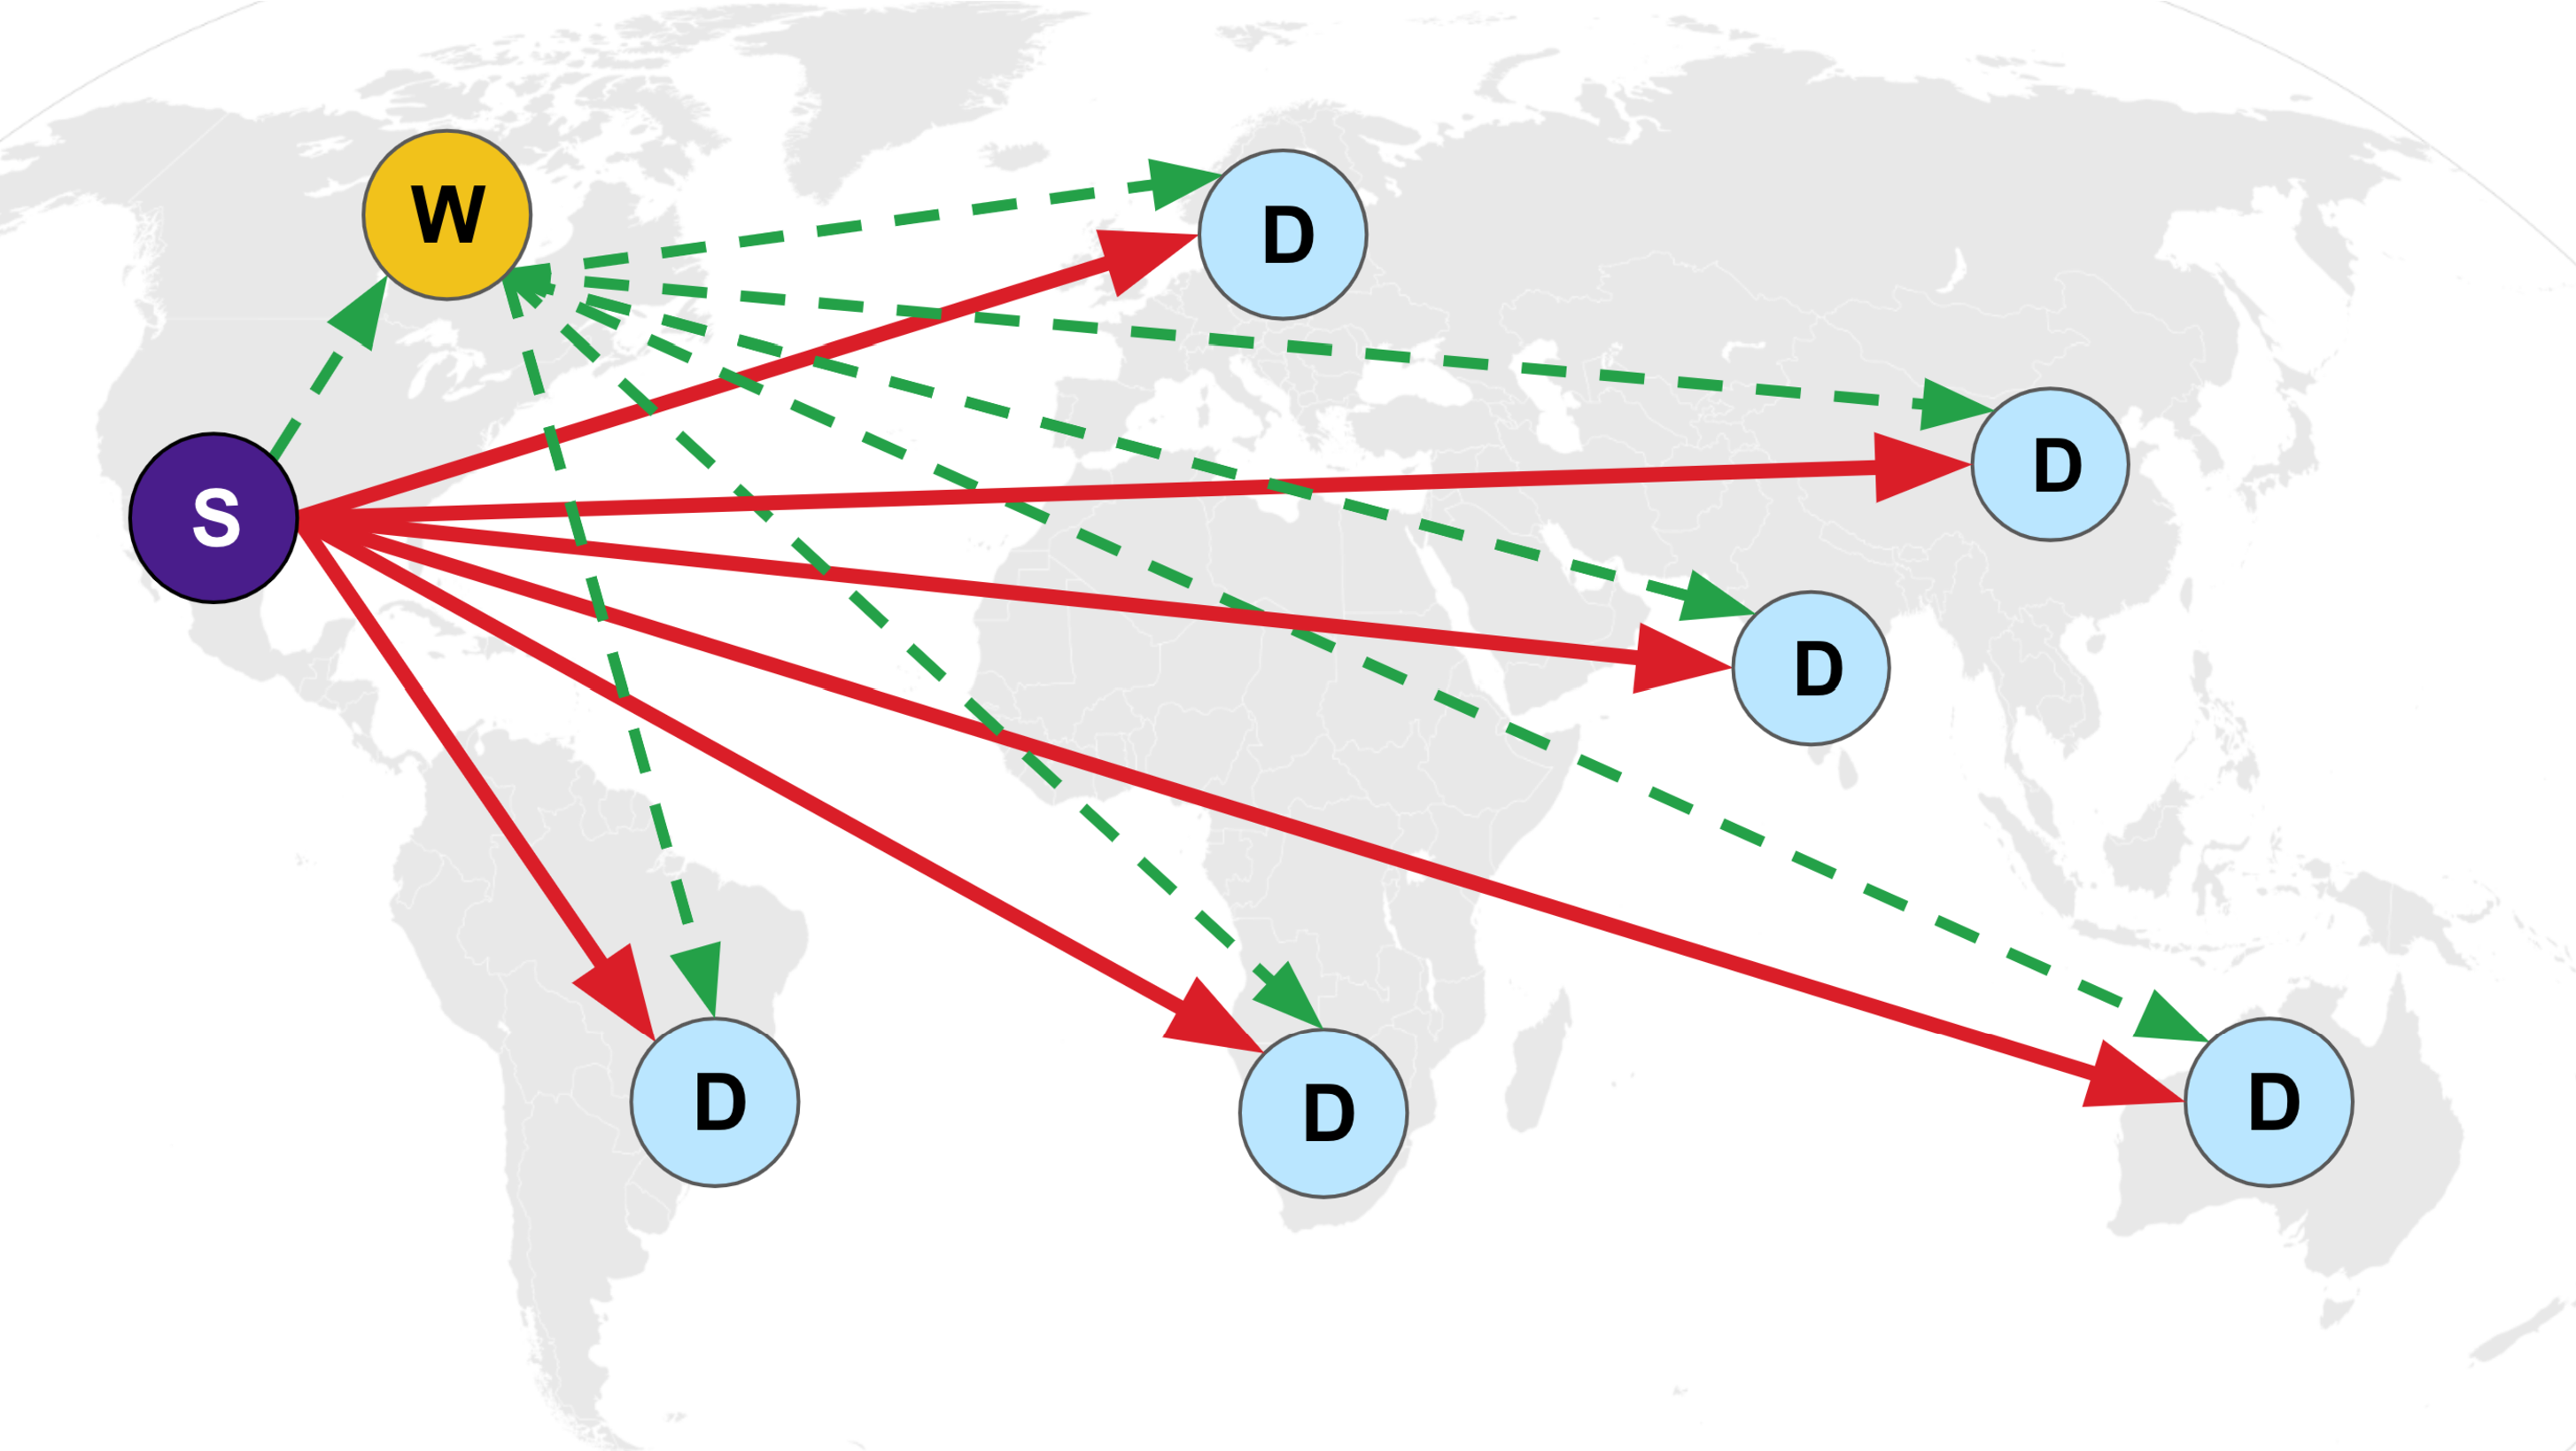
\includegraphics[width=0.8\linewidth]{figures/overview.pdf}
     \caption{Direct replication from a source region (purple) to destination regions (blue) may traverse expensive or slow links, which can be avoided via \textit{waypoint} regions (yellow).}
     % \joey{can we add some more waypoint regions to this plot?}
     \label{fig:overview}
\end{figure}


Egress costs can vary by orders of magnitude depending on the source and destination~\cite{cloudflareegress}, as well as the capacity of cross-region links.
%nd the performance of cross-region links is similarly variable.
%Focusing on throughput alone can, thus, lead to poor results, especially as the number of destinations increases.
As a result, the structure of the multicast replication tree (i.e., what data is replicated along which paths) can dramatically affect the end-to-end throughput and monetary cost of replication.
%
As a concrete example, consider replication from a GCP source region to six AWS regions (Figure \ref{fig:overview}).
%
Direct replication of the data between the source and each destination region (shown in red arrows) would cost $\$720$ per TB. 
%
Instead, replicating to an AWS region with the lowest cross-region egress fees once and multicasting data from that AWS region to other regions (shown in dotted green arrows) would reduce the price to $\$240$ per TB.
%
Further modifying the multicast tree to utilize high-throughput links and offload egress bandwidth from the source node can also improve throughput.

In this work, we solve the problem of \emph{high-throughput, cost-optimized cloud multicast} in which we minimize the cost of data replication while achieving a target replication time (across all destinations) for bulk multicast replication.
%
Cloud multicast incurs costs from network egress fees and compute resources needed to mediate the transfer.
%
In addition, cloud multicast must meet application Service Level Objectives (SLO) for the replication time, such as providing freshness guarantees on replicated data.

We design an optimizer to determine a multicast tree structure given a user-specified source region, destination regions, and target replication time.
By providing varying target replication times, our optimizer can generate a Pareto-curve (shown in Figure \ref{fig:simulated-baselines}) that improves replication cost and throughput compared to prior approaches for cloud multicast \cite{garcia2015cost, ganguly2005fast}. We achieve this by leveraging techniques such as striping, VM parallelism, and overlay networking, while also accounting for the cloud providers' network characteristics, resource constraints, and per-GB network pricing model.

%The key insight in this work is that we can leverage the elasticity of the cloud to design overlay networks of ephemeral virtual machine (VM) waypoints that optimally navigate the path-dependent cloud pricing model to reduce multicast costs and improve throughput significantly. %\joey{I revised this some.}

% Studying the pricing models, resource constraints, and network characteristics of modern cloud providers, we identify opportunities for better multicast tree construction.
% % in cloud replication. 
% We exploit these opportunities using overlay networking techniques to transfer data through ephemeral \textit{waypoint} VMs 
% that are neither the source nor the destination 
% % and may even be in different regions of the world 
% as shown in Figure \ref{fig:overview}.
% We show that the strategic introduction of these waypoints can reduce the overall price of multicast data replication despite using more network bandwidth. % than necessary. 
% %
% Unlike the traditional overlay settings, the cloud offers significantly more flexibility in the number and the location of overlay nodes, as cloud VMs can elastically be instantiated in specified cloud provider regions.


%Our key insight is that transferring data through additional \textit{waypoint} regions, i.e., neither source nor destination regions, can reduce the overall price of multicast replication despite using more network bandwidth than necessary.
%We route data along these price-minimizing replication trees by creating an \textit{overlay network} across cloud regions and providers, which allows us to control the regions and links data traverses through. 

%The cloud context introduces several new challenges: First, cloud pricing for compute and network resources must be considered. Second, cloud resource elasticity enables flexibility in the number of overlay nodes and their location (i.e. on which cloud provider and in which region an overlay node is placed). Third, cloud networks typically have predictable, stable cross-region throughput \cite{jain2022skyplane} and also impose artificial network constraints on VMs, which should be accounted for when designing high-throughput distribution trees.


Designing this optimization is challenging for two main reasons. 
First, the optimizer must account for path-specific pricing models, resource constraints, and varying performance across cloud providers. Existing techniques that formulate the optimization problem in terms of bandwidth allocation cannot be adapted to account for per-GB network pricing without making the problem non-linear (described further in \cref{sec:optimization}). 
%Cloud providers' per-GB network pricing model cannot be easily adapted to prior work optimizing bandwidth-based network costs, which we explain further in \cref{sec:optimization}. 
% to model and optimize multicast price and throughput effectively. 
Second, the optimization search space is combinatorially large, as the optimizer must determine both the set of overlay waypoint regions (regions which are neither the source nor destination) as well as how data will be routed along the overlay network. % (i.e., in the source, destination, and waypoint regions) 
Unlike the traditional overlay settings, the cloud offers significantly more flexibility in the number and the location of overlay nodes, as cloud VMs can dynamically be instantiated in specified cloud provider regions. Furthermore, replicating subsets of data (i.e., stripes) via different paths is critical for achieving high-throughput \cite{castro2003splitstream}.
We introduce several approximations (e.g., pre-selecting the regions and limiting path lengths) to reduce this search space and enable the optimizer to run within seconds.

To run overlay multicast across clouds, we develop \textit{Cloudcast}, a system for bulk data overlay multicast across GCP, AWS, and Azure.
%
Cloudcast has a centralized control plane that supports pluggable algorithms for determining the number and location of overlay nodes and replication trees for multiple segments of data. 
%
We implement our optimizer as well as several baseline algorithms as part of Cloudcast's control plane. 
% We then develop a lightwe % simon: i comment this line out because of the fragment
We run system experiments to multicast data across clouds and show that \sys is able to achieve up to $62.4\%$ cost savings and $2.84\times$ replication speedup depending on the control plane algorithm (Figure \ref{fig:inter-cloud-1}).  

We run an end-to-end system evaluation comparing \sys with  BitTorrent \cite{facebook-bittorrent} and AWS's commercial offering for multi-region bucket replication \cite{awsbucket}, which, like most cloud data replication offerings, only supports replication into or within that cloud.
% 
We find that \sys achieves $7.7\times$ replication speedups and $28.4\%$ cost savings compared to BitTorrent (Figure \ref{fig:p2p_comparison}). Compared to multi-region bucket replication, we find that \sys achieves up to $61.5\%$ cost reduction and $2.3\times$ replication speedup (Figure \ref{fig:aws_comparison}).

%\sys will be open-sourced upon publication. We provide an anonymized tool to explore \sys's optimizer.\footnote{An anonymized website visualizes Cloudcast-optimized overlays for different configurations: \url{https://anon-eurosys-585.github.io} \textcolor{red}{CHANGE ME!!!!!!!!!!!!!!!!}}

\vspace{0.5em}
To summarize, we make the following contributions: 
\begin{compactenum}
    %\item We introduce the problem of \textbf{cost-optimized} cloud multicast and characterize key aspects of cloud pricing models and resource limits that determine optimality.
    % \vincent{missing something about insights into cloud pricing patterns.  More generally, I think something you'll want to push how the structure of clouds and their pricing patterns impacts the optimizer design (to defend against the `it's just an ILP' criticism.}
    
    \item We design an optimizer for minimizing replication cost under replication time constraints. 
    \item We introduce several approximations to reduce the search space for the optimizer, reducing the solver runtime from hours to seconds.
    
    \item We build \sys, an open-source system for cloud overlay multicast with pluggable data transfer policy.
    % \sarah{add footnote}\joey{I think we can skip it for space.}
    %\item We use our optimizer to analyze how cloud pricings affect the cost-minimizing topology solution, especially how future changes on network pricing models (e.g. zero inter-cloud egress) may create new optimization opportunities.
\end{compactenum}


%\ion{Let's be consistent. We are using "dissemination", "distribution", "replication", etc. Let's just use "data replication" everywhere as it has the clearest semantics.} \simon{I fixed it for the intro only.}

% Ion: also consider the priodict solution (less distribution trees) 

% tell Ion when its ready - probably next weekend 
% give eval by sunday 
% evaluation for all stripes versus some of the stripes 
% see difference between the algorithms 

%\section{Background}
\label{s:background}


% merge this with section 3 
% title: problem? price optimized multicast? 
% problem statement? 
% 1. cloud pricing/resources 2. challenges 3. simple example 

\ion{Only the last two sections fit in a background sections, i.e., cloud pricing and resource limits. The rest should be part of related work. So maybe split them in a relatd work and background section. (Remember that a background section typically introduces concepts and lays the ground for the rest of the paper.}

%In this paper, we consider the problem of bulk data transfer from one to many cloud regions, which is at most on the order of ~100s of destinations. 
%Bulk data dissemination over the WAN is a well-studied area, with many application-level multicast algorithms such as 
%Many de-centralized approach to data-dissemination have also been proposed, though these are less relevant since they typically suffer reduced performance and higher complexity to support scaling to millions of destinations, which is not necessary in our scenario. 






%\subsection{High-Throughput Data Distribution}

%\subsection{Cloud pricing models}
%\label{ss:cloud-pricing}
%\subsection{Cloud data replication}


%%%%%%%%%%%%%%%%%%%%%%%%%%%%%%%%
%\subsection{Cloud data replication}
%%%%%%%%%%%%%%%%%%%%%%%%%%%%%%%%

%Bulk data dissemination and data multicast are well studied areas. Recent work from \cite{sima2022ekko} \cite{flinn2022owl} introduced systems for low-latency, bulk replication across datacenters. Prior work in multicast and overlay networking has extensively explored how high-throughput distribution trees can be built for efficiently disseminating data. Cloud data replication is supported by a variety of cloud services, such as AWS DataSync and cross-region replicated buckets, which automatically replicate written data from a bucket in one region to one or more buckets in other regions. However these services have limited support for cross-cloud data movement, and do not optimize the distribution topology to minimize egress costs even from intra-cloud data movement. 

%Rather than relying on just cloud networking, we use cloud VM instances to create an overlay network over cloud networks. Creating an overlay network to optimize cross-clouds transfers was introduced by recent work in Skyplane \cite{jain2022skyplane}. Transferring data with VMs is subjected to artificial network egress/ingress limits imposed on VMs by cloud providers. For example, AWS limits cross-region egress to 5Gbps per VM. Since the limits are imposed per-VM, the per-region limits can be increased by increasing the number of VMs per-region. However additional VMs will incur additional costs, and cloud providers also limit the number of VMs that can be created per-region, so per-region ingress/egress is not infinite. 

%Cloud networks throughput is also highly dependent on the region pairs that data is being transferred between. For example, generally intra-cloud transfers are much higher throughput than inter-cloud transfers, which must go over the WAN. Even intra-cloud transfers can vary in throughput, as show in \ref{fig:tp_heatmap}. However, prior work in Skyplane \cite{jain2022skyplane} showed that throughput profiles between cloud region pairs are fairly stable over 24-hour periods, so can be used to inform a static planner that routes data over high-throughput links. 

%Bulk data dissemination and data multicast are well studied areas. Recent work from \cite{sima2022ekko} \cite{flinn2022owl} introduced systems for low-latency, bulk replication across datacenters. Prior work in multicast and overlay networking has extensively explored how high-throughput distribution trees can be built for efficiently disseminating data. 


%Prior work in Skyplane \cite{jain2022skyplane} optimized point-to-point transfers creating a VM overlay network to route data along high-throughput, low egress-cost links. Skyplane showed that network throughput between region pairs across cloud providers is fairly stable over a 24-hour period, so these profiles can be used to design a static planner that routes long-distance transfers around slow links via overlays. Although Skyplane incorporates both cloud pricing and cloud network characteristics to create optimized point-to-point transfer plans, the optimizer cannot be extended to support multi-destination replication as the identify of partitions of data is not represented in the optimization. Furthermore, Skyplane's implementation does not support multiple destinations and cannot be easily modified to due so, as it does not support sending specific sub-partitions of data specific destinations. \sarah{too much detail?}









% In this paper, we present \sys, a system for bulk data broadcast across cloud regions and providers that utilizes the above insights to discover and implement substantially more efficient data transfers.

% At a high level, \sys allows users to ingest data at a source region using a modular set of connectors (e.g., a VM's filesystem or cloud object store) and broadcast it to one or more destination regions/providers.
% Users of \sys supply the source and destination(s) along with a target transfer completion latency.
% The \sys planner then automatically computes an ideal broadcast topology and executes the transfer accordingly.
% \sys's design, therefore, consists of two primary components:

% \begin{vitemize}
% \item A framework for the elastic instantiation of an overlay network of VM instances that is both highly performant and programmable for easy reconfiguration.
% \item A solver that considers a full range of possible overlay configurations to derive optimized strategies given user objectives.
% \end{vitemize}

% %In order to evaluate different topologies, we design \sys{} to support programmable broadcast topologies.
% %The overlay networks that \sys instantiates \todo{...}
% %To support different broadcast topologies, \sys{} creates an overlay network of VM instances in specific cloud provider regions to relay data.
% %Broadcast topologies assign different sub-partitions of the data to different paths along the network, so \sys{} needs to be able to route specific sub-partitions of the data over specific paths along the overlay.

% Note that although \sys{} is designed for one-off bulk data broadcasts, it can be extended to continual replication via repeated broadcasts of diffs in a straightforward fashion.
% We leave a full exploration of that use case and potential domain-specific optimizations to future work.

% %determines a broadcast topology and deploys an overlay topology of application-space routers (overlay routers) running on cloud VMs to create this network topology.
% %that supports programmable broadcast topologies, including an ILP optimizer for minimizing cost under runtime constraints.

% \section{Motivation}
\section{Problem Setup}
% \todo{rename throughput profiles -> bandwidth profiles}
%Overlay multicast in the cloud presents a number of new considerations, such as cloud pricing models for networking and compute resources as well as resource constraints (e.g., instance limits, per-VM egress limits) imposed by providers.

We frame the problem of cloud multicast in terms of constructing an overlay network for replicating data, which involves defining:
% 
(1) the set of \textit{overlay nodes} (i.e., cloud VMs) and (2) the \textit{paths} between those nodes that will be included in a multicast replication tree.
% 
\sys eventually divides the target data into multiple \textit{stripes} (i.e., partitions), so concurrent replication trees may be used in a single transfer.
%\sarah{I wonder if we should move this to the intro, or if its too much detail?}
%VL: See note in intro
Our optimization objective is to minimize the monetary cost of replication while also meeting a replication time constraint.
%
%The time constraint is critical as many applications require a Service Level Objective (SLO) on the transfer completion time.
% 
%For example, disaster recovery requirements may aim to copy data to multiple clouds within a bounded time to minimize data unavailability upon an outage.
% 
%As a reference point, AWS Replication Time Control offers a 15-minute transfer completion time SLO~\cite{aws-replication-time-control}.
%
%VL: below is redundant
%Multicasting data with sufficient throughput and minimal cost requires balancing these two concerns using
% the above knobs, i.e., 
%the number and location of overlay nodes and paths.
%we must select the number and location of overlay nodes and the paths that data is replicated to achieve the right balance between replication cost and throughput.

% In the remainder of this section, we describe the characteristics of the cloud that are relevant for cost-optimizing cloud multicast. 

% The cost-optimized cloud multicast problem is fundamentally different from the classic network multicast problem:
% \begin{enumerate}
%     \item Variable egress pricing by source and destination
%     \item Variable network bandwidth by source and destination
%     \item Elasticity to mitigate source-region egress limits
% \end{enumerate}

% We explain each difference in isolation then illustrate the full problem space with a simple example.

\begin{figure}[tbp]
     \centering
     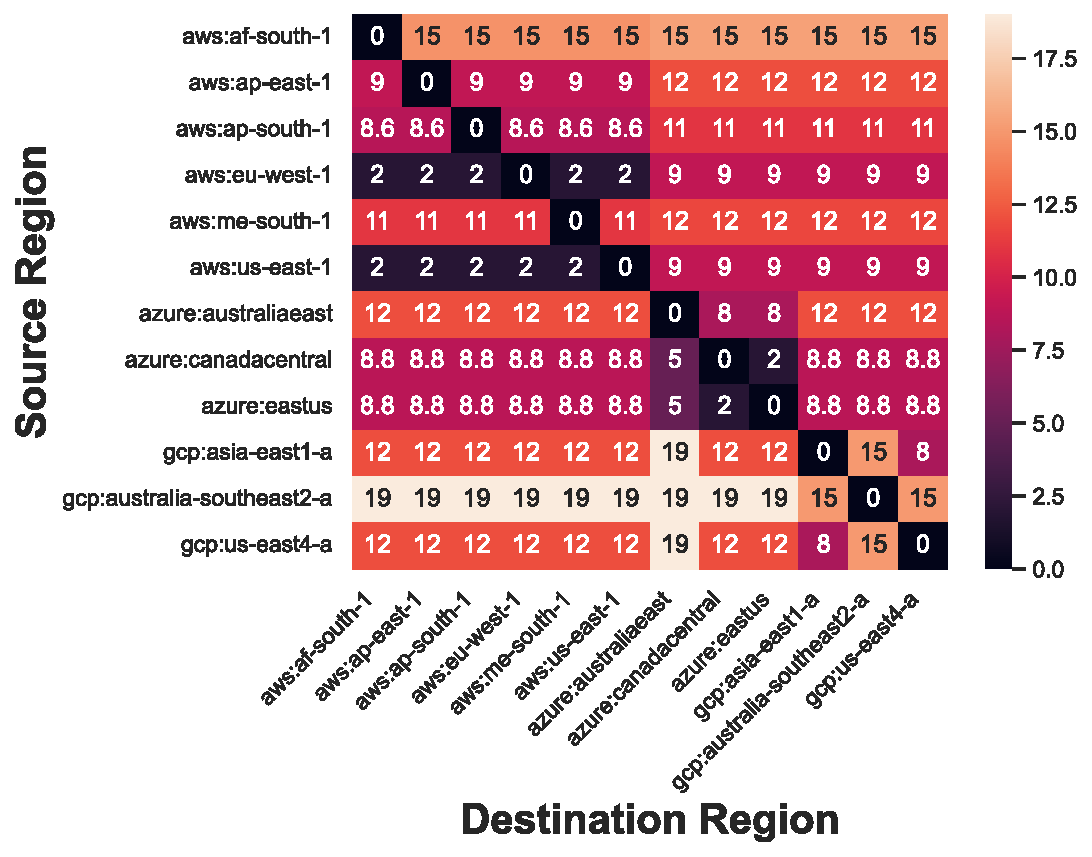
\includegraphics[width=0.9\linewidth]{figures/cost_heatmap.pdf}
     %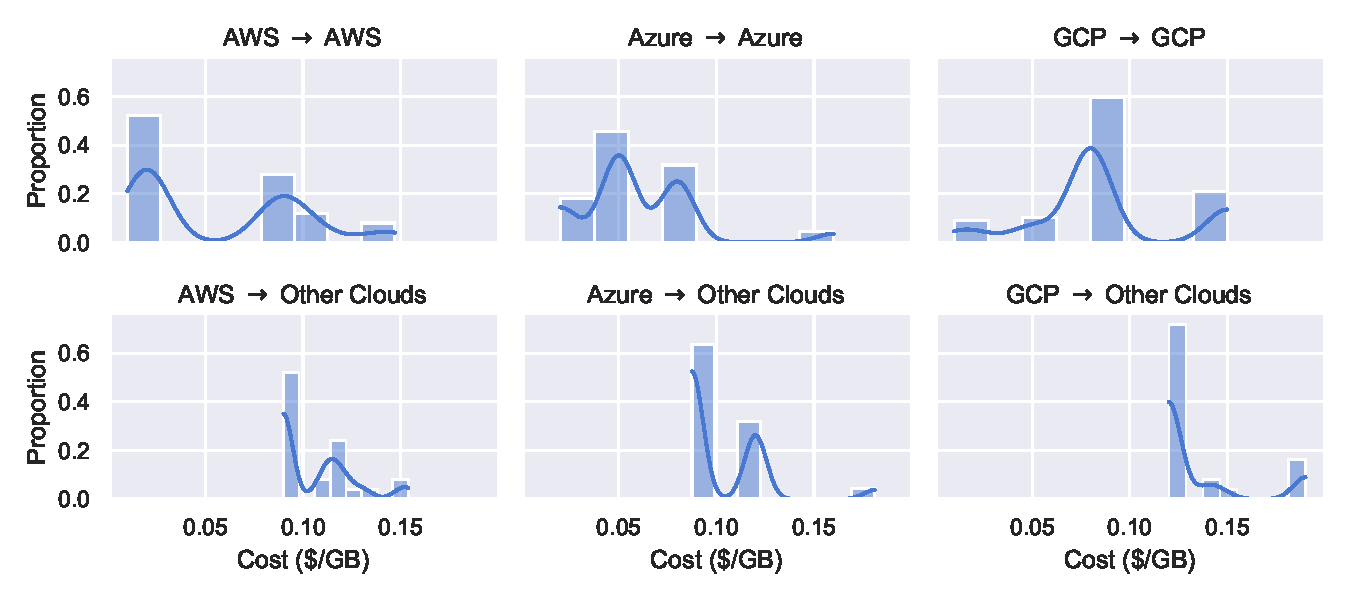
\includegraphics[width=\linewidth]{figures/2-3-cost-histograms.pdf}
     \caption{Egress fees between regions (in cents per GB).}
     \label{fig:cost_heatmap}
\end{figure}
% \sarah{explain setup of we want to transfer data across regions - and then explain how we can use VMs to transfer data, and now we want to decide on that overlay structure}
\subsection{Egress Costs}
A unique aspect of multicast in the cloud is the effect of egress costs incurred for data transferred across cloud regions.
%
Cloud providers charge for wide-area data transfer \textit{per-GB} of data transferred.
% 
Egress prices---as a method of keeping data within the provider's regions without disincentivizing migration into the provider---dominate data movement costs in the cloud and fundamentally change the multicast problem.
% \vincent{how? give some intuition}\joey{I think this is addressed in the figure but we could/should do better for the camera ready.}
% 
Figure \ref{fig:cost_heatmap} visualizes the pricing for 11 regions across AWS, Azure, and GCP.
% 
Prices vary depending on the source and destination cloud or region, with differences of up to $23\times$ across region pairs.
%
Along those lines, one particularly important axis is whether the transfer stays within a given cloud provider or crosses provider boundaries, as inter-cloud egress costs are generally higher than intra-cloud egress.



Intra-cloud egress (data movement between geographically separated datacenters in the same cloud provider)
% , at the time of writing, 
is priced between $\$0.01-\$0.19$ per GB transferred.
% 
Prices typically increase with longer-distance transfers.
% 
For example, GCP charges $\$0.08$ for transfers between continents but only $\$0.02$ for transfers within the US.
% 
Some smaller providers (e.g., IBM, Cloudflare) offer free cross-region egress.

Inter-cloud egress (data movement between different cloud providers) is typically priced at a much higher rate per GB ($\$0.08-\$0.23$).
% 
As such, it is essential to minimize cross-cloud transfers in a multicast replication tree.

\begin{figure}[tbp]
     \centering
     % 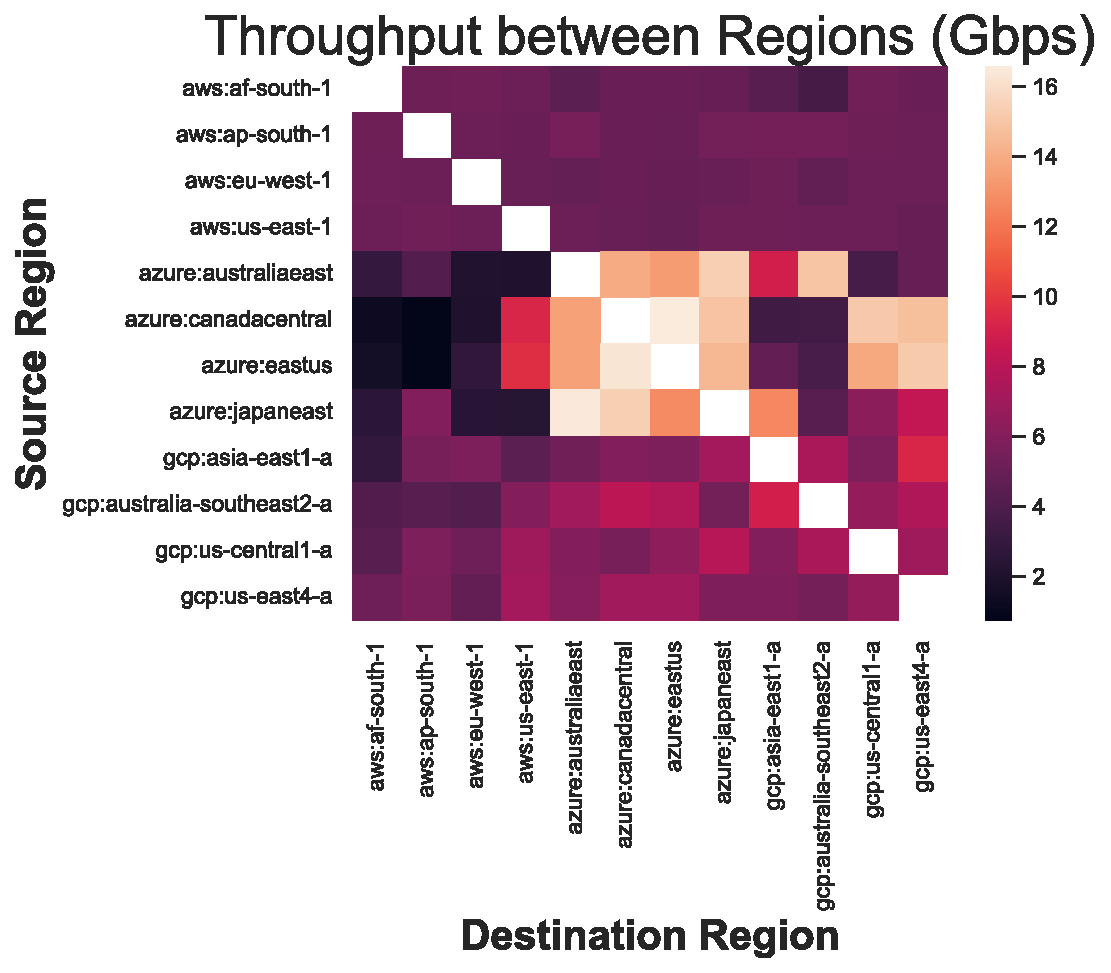
\includegraphics[width=\linewidth]{figures/tp_heatmap.pdf}
     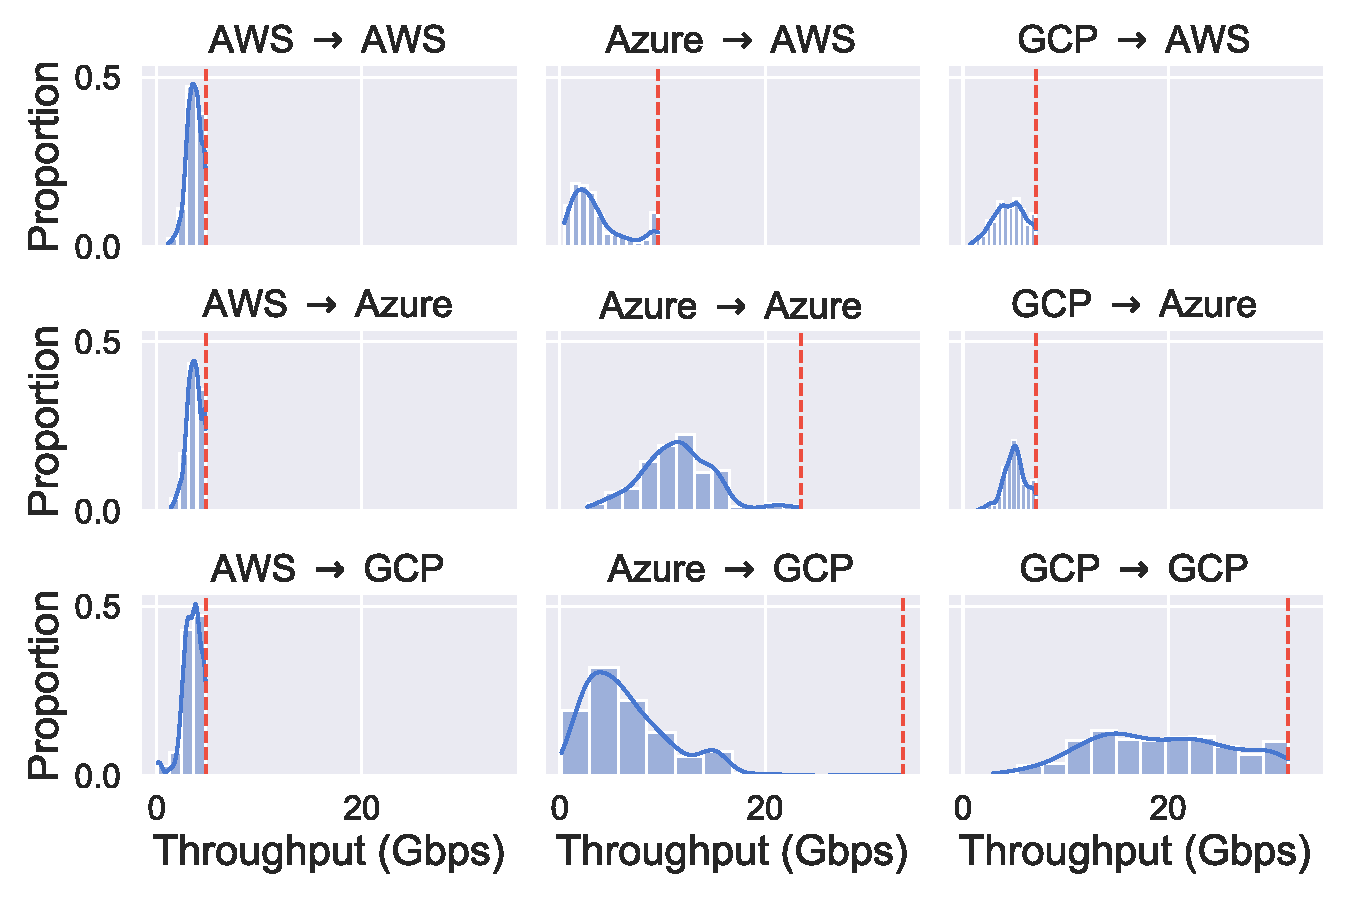
\includegraphics[width=0.9\linewidth]{figures/3-3-throughput-histograms-no-share-x.pdf}
     \caption{Bandwidth distribution (in Gbps) between regions. Per-VM egress limits are marked in red dotted lines.} %Bandwidth varies significantly across regions and providers. 
     %AWS limits cross-region egress to 5\,Gbps, so have lower throughput generally. 
     %Azure has high intra-cloud performance but poor performance in the AWS region, except for AWS US East 1.  
     % \todo{Align X-axis to show variation between providers} 
     % \shu{Also the x and y title here is too small} \paras{Show the throughput wall with markings to show infeasible region.}
     \label{fig:tp_hist}
\end{figure}

\subsection{Bandwidth Variability Across Endpoints}
\label{ss:bandwidth-variability}
Meeting replication time constraints can be challenging due to network bandwidth variability in the cloud.
One type of variability arises from cloud providers, who impose constraints on per-VM egress and ingress bandwidth.
These constraints differ significantly across providers:
for instance, AWS throttles intra-cloud and inter-cloud egress to 5\,Gbps per VM, while Azure imposes no VM-level limits.
The impact of these egress limits can be observed in Figure \ref{fig:tp_hist}, where bandwidth is capped at the VM egress limit for AWS and GCP.
Limited node egress poses a particular challenge for cloud multicast, as the source node's egress bandwidth is often the bottleneck.

Even when source-node bandwidth is not the bottleneck, observed network capacity can also vary considerably across cloud region pairs (up to $202\times$).
%
Note that these networks are relatively stable across time; prior work~\cite{jain2022skyplane} has found that network throughputs are stable over periods of at least 24 hours.
%
Instead, variations are primarily observed across different source and destination regions.
% 
Figure \ref{fig:tp_hist} depicts the distribution of profiled bandwidth between VMs running in AWS, Azure, and GCP.
% \joey{how many pairs and for how long?}
% 
Intra-cloud bandwidth is typically (but not always) higher than inter-cloud bandwidth.
%, as each category has significant variability. 

%Meeting replication deadlines can therefore require carefully choosing the replication tree to both leverage high-bandwidth paths across regions and alleviate the effects of source region bottlenecks.

% However, achieving high throughput for replication can be challenging: First, cloud providers control their network traffic to allocate certain amounts of bandwidth to paths between specific regions, limiting the per-VM throughput between regions. \sarah{there should be a better way to say this} Second, cloud providers also impose artifical limits on the network egress and ingress per-VM. 
% For example, AWS limits cross-region egress to 5Gbps per VM, as shown in \cref{fig:tp_hist}. 

% nb paras: this is a soluton space concern
% Meeting these constraints requires selecting the right waypoint regions, number of VMs, and distribution trees for data. To do so, we must optimize both the number of VMs per-region (the overlay node set) and the distribution trees together.  \sarah{Say something about how this increases the search space?} \simon{addressed in previous paragraph, the latency target is about the constriant right?}

\begin{figure*}[tbp]
    \centering
    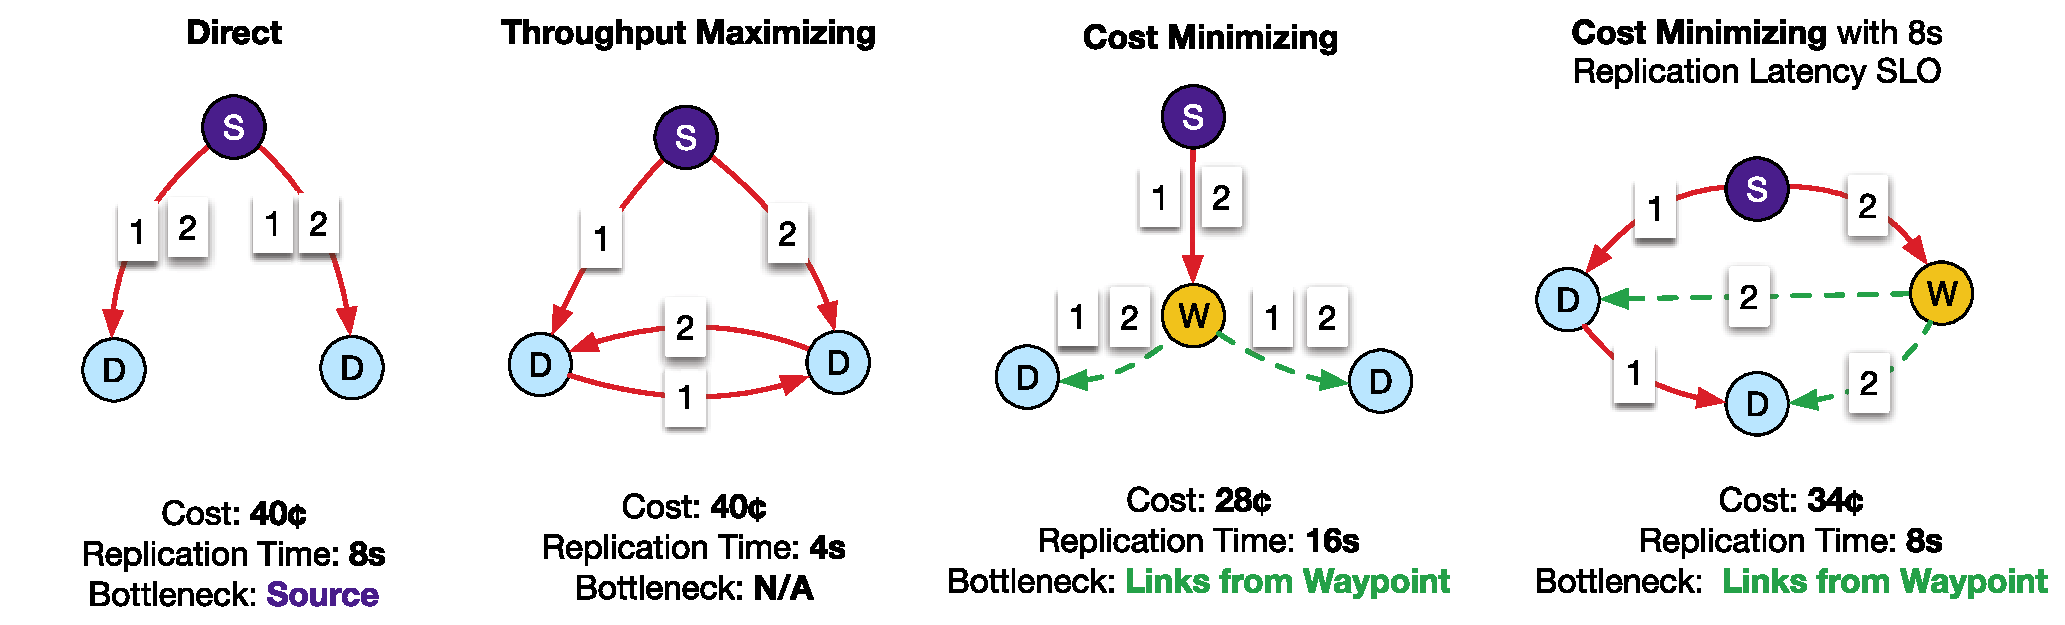
\includegraphics[width=0.9\linewidth]{figures/toy_example.pdf}
    \caption{Overlay node set and distribution trees for a toy example.  The source and destination nodes are marked `S' and `D' respectively, while waypoint nodes in yellow are marked `W'. Expensive, fast paths ($\$0.1$ per GB, $2$\,Gbps) are shown in solid red, while slow, cheap paths ($\$0.02$ per GB, $1$\,Gbps) are shown in dashed green. 
    %In the \textit{Direct} tree, the source node egress (4Gbps) is the bottleneck in sending out 8GB ($4 \times 2$GB stripes) of data, while both the \textit{Cost Minimizing} trees, the outgoing links from the waypoints ($1$\,Gbps) are the bottleneck. For the \textit{Throughput Maximizing} tree, all link bandwidth is used to full capacity (2Gbps) to each send $2$GB stripes, and are not bottlenecked by node egress or other links' bandwidth. 
    \paras{Shouldn't cloudcast be something between 4 and 8s?}
    %\simon{This needs to be move up to earlier pages. This is a good "motivation plot".\sarah{from shu/ion:I got some feedback for the toy example 1) make it more clear on the data size (i.e. putting maybe a small graph right next to those examples showing partition 1/2 aggregate size) and 2) make it more clear on how the replication time is calculated (it’s described in the text and caption, it’s better to have text right next to the link showing what’s the bottleneck bandwidth or something similar to that; make it more intuitive on understanding why the topology is slow)}}
    } 
    \label{fig:toy_example}
\end{figure*}
\subsection{Elasticity of Resources}

%In the multicast setting, source region bandwidth is often a bottleneck.\sarah{this doesn't fit together with the title of the section - need a transition} 
% 
%Prior work like Splitstream~\cite{castro2003splitstream} note this bottleneck with proposed solutions in non-cloud environments.
% 
A major advantage of the cloud is resource elasticity and the ability to flexibly provision VMs across many regions. 
% 
In the face of the source bottlenecks described above, VM elasticity translates to a corresponding \emph{elasticity of bandwidth}.
%
% In other words, 
Allocating multiple parallel VMs enables users to scale throughput beyond per-VM network bandwidth limits.
%
% This is notionally similar to prior work in peer-to-peer overlays (e.g., Splitstream~\cite{castro2003splitstream}) that leverage sharding for performance. \sarah{I dont understand what this means. weren't we jsut using this to reference evidence for source bottlenecks?}\joey{I think the above statement is risky since it relates but doesn't contrast... maybe we comment it out for now?}

%These VMs can be deployed at the source region to directly reduce the impact of source region bottlenecks, which are common in the multicast-setting: for example, prior work like Splitstream~\cite{castro2003splitstream} note this bottleneck with proposed solutions in non-cloud environments.

Unfortunately, adding elastic VM capacity at the source region has limitations.
% 
Additional VMs add additional costs due to per-second billing on VMs, which can impact the cost/throughput tradeoff.
% 
We note that because the marginal cost of additional VMs is often relatively small compared to egress fees, the tradeoff is often worth making.
%it is often possible to significantly increase throughput at only a small marginal increase in cost --- in the cloud, fast can be cheap.
% 
However even in these situations, bandwidth elasticity has limits: for instance, if a network-based bottleneck is unavoidable or when cloud providers limit the number of vCPUs per region. 

%\sarah{maybe better to start with this?} 
Crucially, elastic VM capacity can also be deployed at \textit{waypoint regions} that are neither the source nor the destination.
% 
These waypoint regions can help mitigate source VM bottlenecks by distributing load from multicast fan-out across multiple separate regions.
% 
Waypoint regions also mitigate 
% intermediate 
points of congestion 
% in a transfer 
by routing data around slow paths.
\subsection{Illustrated Example}
Selecting overlay nodes and replication trees to optimize cost and throughput is challenging.
Consider the toy example in Figure \ref{fig:toy_example} for a 2\,GB replication with two 1\,GB stripes.
Assuming a 4\,Gbps bandwidth limit for all nodes and one VM per region, the source (``S'') and destination (``D'') nodes have fast but expensive outgoing paths, capable of sending at 2\,Gbps but costing $10\mbox{\textcent}$ per GB transferred.
Other regions have cheaper but slower outgoing paths, capable of sending at 1\,Gbps but costing $2\mbox{\textcent}$ per GB transferred.
In a simple direct replication scenario, the replication will be bottlenecked by the source node's egress limit (4\,Gbps). With two copies of data to send, the total transfer time will be 8 seconds.

Like many bandwidth-optimized techniques \cite{castro2003splitstream, ganguly2005fast,kostic2003bullet}, we offload egress bandwidth by sending a single data copy from the source and leveraging multiple replication trees. Replication cost is reduced by replicating to a waypoint, and then multicasting to destinations. This doubles replication time to 16 seconds due to stripes being replicated via the slower path (dotted arrows). An 8-second replication SLO is met by transferring just one stripe via the cheaper waypoint.

This simple example presents a large search space for possible replication trees, and real-world cloud networks present additional parameters such as choosing the number of VMs per region and many possible waypoint regions.

%\section{Motivation}




%Overlay multicast in the cloud presents a number of new considerations, such as cloud pricing models for networking and compute resources as well as resource constraints (e.g., instance limits, per-VM egress limits) imposed by providers.

\begin{figure}[t]
     \centering
     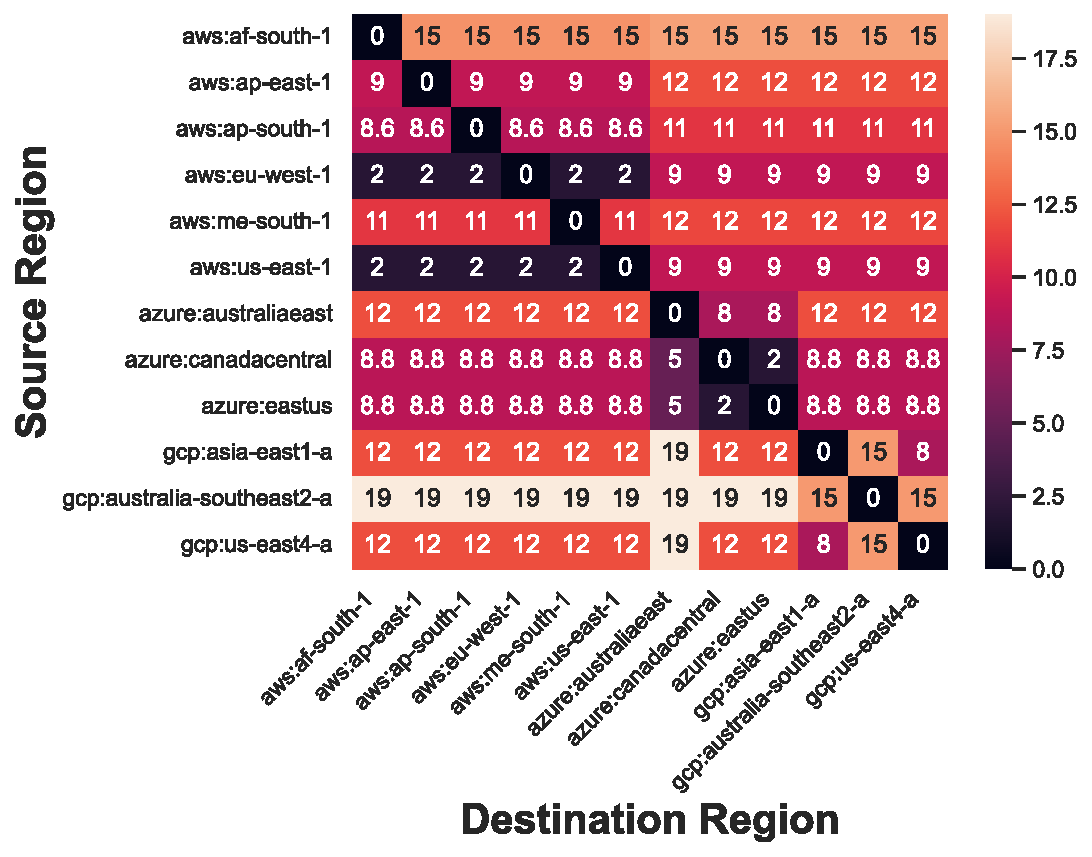
\includegraphics[width=\linewidth]{figures/cost_heatmap.pdf}
     %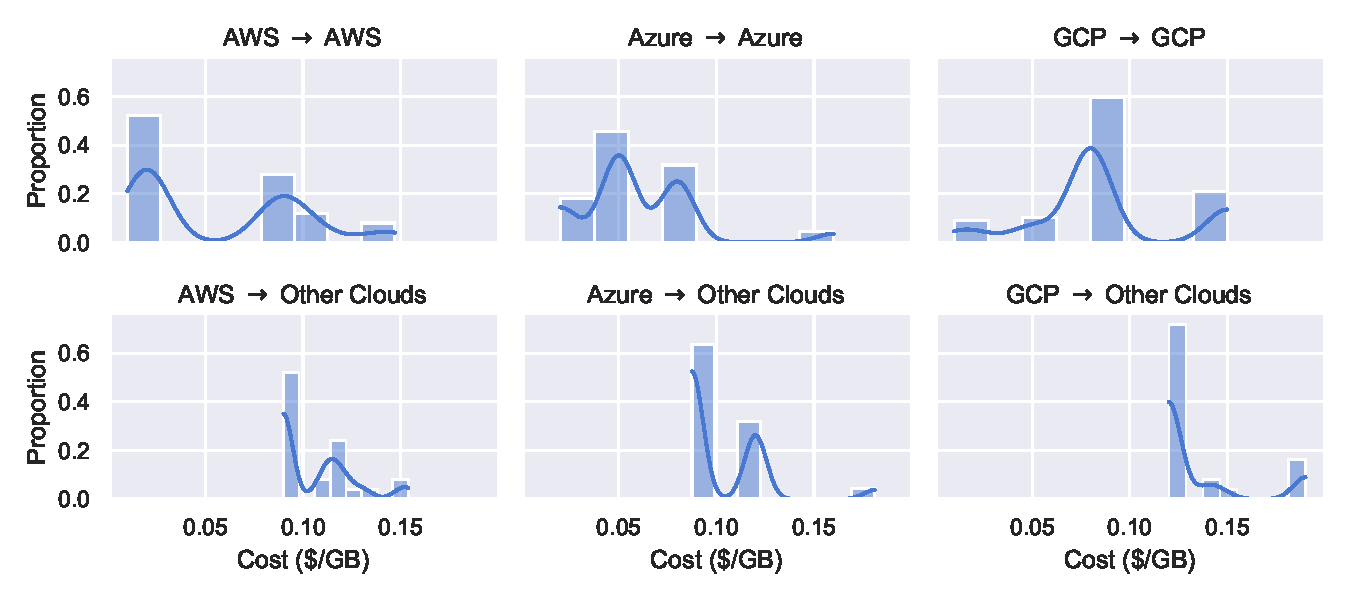
\includegraphics[width=\linewidth]{figures/2-3-cost-histograms.pdf}
     \caption{\textbf{Egress fees between regions (in cents per GB).} Egress fees are generally lower for intra-cloud transfers, but some specific regions have higher baseline egress costs. Pricing across region pairs can vary up to 19$\times$. \todo{potentially change color scheme?} \shu{lighter to represent cheaper}}
     \label{fig:cost_heatmap}
\end{figure}


%To represent the cost of overlay cloud multicast, both the prices of compute and networking resources must be incorporated into the cost. In addition to egress fees, VM instances are charged for their running duration during the transfer. However, egress fees typically dominate VM costs (up to $20\times$ for inter-cloud links).



%%%%%%%%%%%%%%%%%%%%%%%%%%%%%%%%
\subsection{Challenges of Multicast in the Cloud}
%%%%%%%%%%%%%%%%%%%%%%%%%%%%%%%%
 %Each of these considerations can vary across providers, as pricing models and resource constraints are heterogeneous~\ion{what is the difference between "heterogeneous" and "vary across providers"? Just use the same terminology.} across clouds. As a result, optimizing multicast price and replication time can be complex. 

\begin{figure*}[t!]
    \centering
    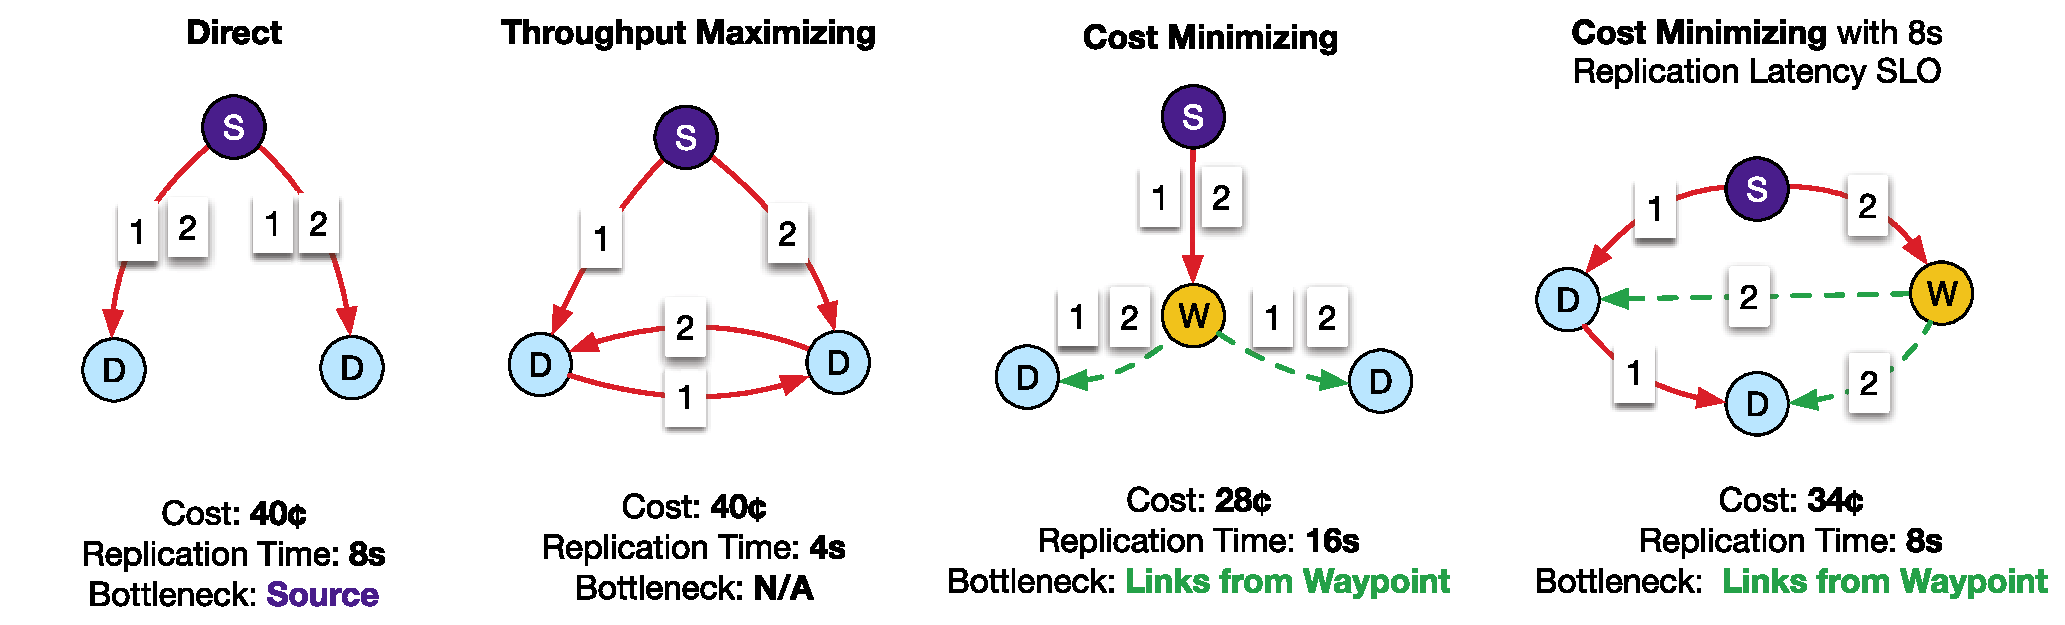
\includegraphics[width=.85\linewidth]{figures/toy_example.pdf}
    \caption{\boldmath Overlay node set and distribution trees for a toy example:  The source and destination nodes are marked `S' and `D' respectively, while waypoint nodes in yellow are marked `W'. Expensive, fast links ($\$0.1$ per GB, $2$\,Gbps) are shown in solid red, while slow, cheap links ($\$0.02$ per GB, $1$\,Gbps) are shown in dashed green. In the \textit{Direct} tree, the source node egress (4Gbps) is the bottleneck in sending out 8GB ($4 \times 2$GB stripes) of data, while both the \textit{Cost Minimizing} trees, the outgoing links from the waypoints ($1$\,Gbps) are the bottleneck. For the \textit{Throughput Maximizing} tree, all link bandwidth is used to full capacity (2Gbps) to each send $2$GB stripes, and are not bottlenecked by node egress or other links' bandwidth. 
    %\simon{This needs to be move up to earlier pages. This is a good "motivation plot".\sarah{from shu/ion:I got some feedback for the toy example 1) make it more clear on the data size (i.e. putting maybe a small graph right next to those examples showing partition 1/2 aggregate size) and 2) make it more clear on how the replication time is calculated (it’s described in the text and caption, it’s better to have text right next to the link showing what’s the bottleneck bandwidth or something similar to that; make it more intuitive on understanding why the topology is slow)}}
    } 
    \label{fig:toy_example}
\end{figure*}

% \vincent{This subsection seems to duplicate the information of the previous subsection.  I would suggest merging 2.1 and 2.2 (move the first paragraph of 2.1 into 2.0 and make 2.1 a unified "challenges" subsection).  If you really wanted to keep them separate, I think 2.2 needs to be much shorter and punchier.}


 

%At the same time, there is an opportunity in the flexibility offered by the cloud: cloud elasticity can be used to allocate a variable number of overlay nodes in specific regions to improve multicast tree performance and throughput. In this section, we describe the challenges in modeling and optimizing multicast cost. 

Cloud data replication presents several new considerations compared to traditional multicast scenarios, many stemming from the unique ways in which modern providers manage and restrict resource utilization. 

\heading{Price of multicast in the cloud}  One way in which providers manage resource utilization is through pricing.
%Cloud providers offer a variety of services, with different pricing models applied to different services.
For example, Virtual Machines (VMs) are priced based on  \textit{per second} of virtual machine usage, while networking resources are priced \textit{per unit volume} (GB) of the data transferred and depend on whether the data is crossing region or cloud boundaries.
Different cloud providers have varying pricing models, but typically networking within the same region is free, while data egress out of the cloud is charged at the highest rates. Cross-region egress (data movement within the same cloud provider) is charged somewhere in-between, with some providers (e.g., IBM, Cloudflare) offering free cross-region egress but other clouds (e.g., AWS, GCP, Azure) charging between $\$0.01-\$0.19$, depending on the source and destination region (shown in \cref{fig:cost_heatmap}). For example, GCP charges $\$0.05$ for transfers in/out of Asia regions but $\$0.02$ for US regions.


Why is it challenging to integrate pricing information into multicast?
% 
First, conventional formulations of the problem only consider allocating throughput between regions.
% 
However, egress fees in the cloud are priced according to data volume (i.e., \$ per GB) instead of throughput (i.e., \$ per Gbps).
%
Second, overlay multicast relies on the use cloud VM which are price per-second. A such, longer runtimes or the use of additional VMs (e.g. to use additional regions or improve parallism) can result in additional costs that must be co-optimized along side egress costs. 
% 
%Furthermore, cloud VM resources are also subject to per-second fees, which must be considered in selecting the number of overlay nodes created. 
\ion{What is special about "pre-second" fees? The main point here is that they charge per VM instances; I think mentioning "per-second" is a distraction.}
%\sarah{I mentioned this since its the reason why the optimization problem is hard to make linear, but maybe that's too much of a detail..}
% A naive data distribution topology may repeatedly use expensive links unnecessarily, such as when transferring from a high-egress region repeatedly to multiple other destinations instead of transferring the data once to a lower-egress region once and disseminating data to destinations from there. In addition, although cloud resource elasticity can be leveraged to create more VMs to parallelize transfer execution, the additional per-second cost of VM usage must also be modeled as part of the transfer cost.  




% \heading{Elasticity of cloud networks}\ion{This para seems to be about limits rather than elasticity. In my mind elasticity refers to the fact that I can use any number of VMs and I can place waypoints in any region. Elasticity is an opportunity. Still need to mention it because it can significantly increases the search space.}
% From the perspective of tenants, cloud networks are elastic as they can access additional capacity by provisioning more resources (VMs).
% Cloud providers allocate terabits of network links between their cloud regions~\cite{jain2013b4} and run them at high utilization.
% Providers reallocate bandwidth via traffic engineering~\cite{singh2021cost,hong2018b4} to add additional capacity and manage outages.
% Some providers place limits on the elasticity of wide-area networks with AWS and GCP limiting per-VM egress bandwidth to 5 Gbps and 7 Gbps respectively.
% To have sufficient bandwidth between regions, we can increase the number of VMs created per-region. 



\heading{Meeting replication time targets}
In practice, data transfers often have a Service Level Objective (SLO) on the desired transfer completion time.
% \ion{I think these SLOs are per latency (as mentioned earlier) rather than throughput. We need to be consistent.}
% 
It is common to replicate data to a secondary region or cloud to ensure business continuity in case of a cloud outage.
% 
AWS Replication Time Control enables users to request a transfer complete within a fixed 15-minute SLO~\cite{aws-replication-time-control}.
%
However, achieving high throughput for replication can be challenging: First, cloud providers control their network traffic to allocate certain amounts of bandwidth to paths between specific regions, limiting the per-VM throughput between regions. \sarah{there should be a better way to say this} Second, cloud providers also impose artifical limits on the network egress and ingress per-VM. For example, AWS limits cross-region egress to 5Gbps per VM, as shown in \cref{fig:tp_heatmap}. Limited VM egress bandwidth is particularly problematic for multicast, where the source node bandwidth is often a bottleneck. Since the limits are imposed per VM, the per-region limits can be increased by increasing the number of VMs per region, however the number of VMs per region is also subject to limits. 

Meeting these constraints requires selecting the right waypoint regions, number of VMs, and distribution trees for data. To do so, we must optimize both the number of VMs per-region (the overlay node set) and the distribution trees together.  \sarah{Say something about how this increases the search space?} \simon{addressed in previous paragraph, the latency target is about the constriant right?}

%Since these requirements may vary across applications, ideally users can flexibly trade off cost and throughput for cloud multicast. 

% derive the number easily: add the data partition size (make the replication time clear; the cost is clear now but not the time); show the bottleneck, and show how big the block is; assume perfectly pipeline; 

% \begin{figure*}
%      \centering
%      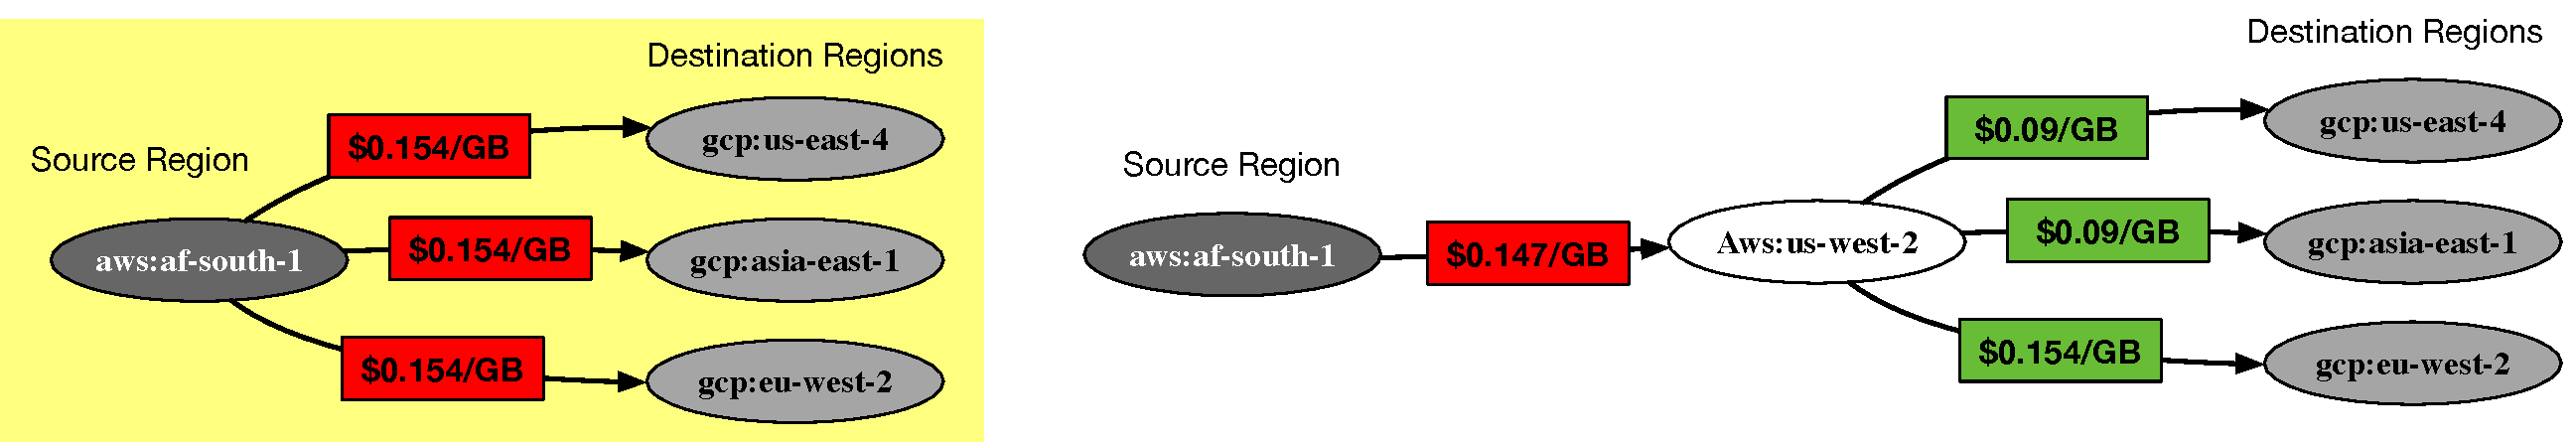
\includegraphics[width=\linewidth]{figures/overlay_example_long.pdf}
%      \caption{\textbf{Cost saving overlay region} Introducing an overlay node can reduce the overall egress cost. In the yellow box, we show a direct topology from an AWS region to three GCP regions that costs $0.462$ per GB transferred. Transferring the data to another AWS region first reduces the overall cost to $0.417$ per GB. \sarah{This is a bad example because you should just transfer to GCP once - change to AWS-only example}}
%      \label{fig:cost_overlay}
% \end{figure*}

\heading{Resource elasticity} A major advantage of the cloud is resource elasticity and the ability to flexibly create VMs across many cloud regions. While the elastic bandwidth means that we can place any number of VMs as waypoints in any regions, it significantly increased the search space for optimization: our optimizer not only controls how data is replicated across the network, but also the number of location of nodes in the network (which we refer to as the \textit{overlay node set}). 

%Cloud providers place limits on the elasticity of wide-area networks. Cloud tenants can access additional network capacity by provisioning more resources (VMs). 

%Cloud providers also impose artificial constraints on networking and compute resources. For example, AWS limits cross-region egress to 5Gbps per VM, as shown in \ref{fig:tp_heatmap}. Since the limits are imposed per VM, the per-region limits can be increased by increasing the number of VMs per region. However, additional VMs will incur additional costs, and cloud providers also limit the number of VMs that can be created per region, so per-region ingress/egress is not infinite. Limited node bandwidth is particularly problematic for multicast, where the source node bandwidth is often a bottleneck. 

%Additionally, we must account for the fact that cloud provider also caps the number of VM in each cloud, as well as pricing the compute in each region at varying rates. 



\subsection{A Simple Cloud Multicast Example}


Optimizing cost and throughput requires the selection of both the right \textit{overlay node set} as well as one or more replication trees along which data is routed. We assume data is divided into multiple \textit{stripes}, i.e. subsets of the data routed along the same replication tree, to allow for multiple concurrent replication trees. 

Consider a toy example shown in \cref{fig:toy_example} for a 2GB replication, where we have two 1GB stripes. For simplicity, we assume that all nodes have a 4Gbps bandwidth limit and we can only have one node per region. The source and destination nodes (grey) have outgoing links which are fast but expensive: each link can send at 2Gbps but costs $10\mbox{\textcent}$ per GB. However, there are other regions that have outgoing links which are cheaper but slow: they can send at 1Gbps, but cost  $2\mbox{\textcent}$ per GB. For a simple direct replication of the data from the source node to the destination nodes, the replication will be bottlenecked by the source node's egress limit (4Gbps). Because the source must send out two copies of the data, the transfer time will be 8 seconds in total. 

First, let's consider how we can optimize the throughput of the replication. We can offload egress bandwidth from the source to the destinations (an insight from \cite{castro2003splitstream}) by only sending out one copy of the data from the source. We show this in the throughput-maximizing solution, where we transfer each stripe via two different paths and peer between the destinations. 

Next, let's consider how we can also optimize the cost.  We can reduce the cost of the replication by replicating data to a waypoint region first, and then multicasting the data to the destinations from the waypoint. However, this increases our replication time by 16 seconds, which may be unacceptably slow. We can meet an 8-second replication SLO by trading off throughput for cost, by only transferring one stripe via the slower, cheaper waypoint region. 

Even for toy example, there are many different possible distribution trees, and this search space exponentially increase with more destinations, partitions, and possible waypoint regions. 

%In this toy example, we use one VM for transfer per region, and each VM has an egress limit of 4 Gbps. We show examples of possible broadcast topologies in \ref{fig:toy_example} for two stripes and two destinations. The replicated data is transferred via two stripes, represented in red and blue. A throughput-maximizing topology \textit{peers} stripes of the data to offload bandwidth from the source. The cost-minimizing solution uses an overlay region with cheaper, but slower connections to the destination regions. A cost-minimizing solution with a replication latency SLO may route part of the data through the overlay, and part of the data directly to the destinations to balance both cost and throughput. 


%\heading{What does it cost?}
%\shu{Rethinking multicast in the cloud, explain more precisely what's happening with cost and edge capacity}

%\heading{Utilizing edge capacity} Utilizing the edge capacity can be challenging due to limited node egress bandwidth. 
\section{Cost Optimization in \sys{}}
\label{sec:optimization}

%\ion{I do not think we need to say "offline" here since we do this optimization per transfer. "Offline" might refer to precomputing a set of possible multicast trees for any possible transfer. The only thing we do not do is recomputing the multicast tree during transfer.}
We design an optimizer to minimize replication cost while meeting a replication time SLO (i.e., a constraint on the maximum replication time to a destination).
Our optimizer has two main contributions.
The first is a Mixed-Integer Linear Program (MILP) formulation of the cost-aware multicast problem, jointly selecting overlay nodes and replication trees. 
% \joey{I rewrote the red sentence below as this sentence:}
% While others~\cite{zhang2018bds} have formulated multicast overlays as MILPs, our approach is fundamentally different both in our objective (cost rather than throughput) and the corresponding framing of the MILP (the space of decision variables).
% sarah: so technically some do model cost
%%% \textcolor{red}{ %\joey{old version}
While others~\cite{zhang2018bds, ganguly2005fast} have used MILP formulations for multicast overlay design, they formulate the optimization problem in terms of \textit{bandwidth}.
Extending these formulations to accommodate per-GB costs would violate linearity as data transfer volume (cost) is proportional to the product of the key decision variables: allocated bandwidth and replication time.
As a consequence, we propose a  new formulation that reframes the optimization in terms of data volume. 
Our new formulation assigns discrete subsets of data (i.e. stripes) to replication paths in the network while ensuring that a complete copy of the data arrives at all destinations.
Unfortunately, solving this MILP formulation can be intractable for larger numbers of destinations.
Our second contribution is an approximation of the MILP formulation that significantly reduces solve time without significantly degrading the solution quality.



\newcommand{\flowmax}[0]{\small{\textsc{bandwidth}}^{path}}
\newcommand{\volume}[0]{\textsc{volume}}
\newcommand{\connectionlimit}[0]{\small{\textsc{Limit}}^{conn}}
\newcommand{\frob}[2]{\langle #1, #2 \rangle}

\newcommand{\dest}[0]{\small{\textsc{dest}}}
\newcommand{\node}[0]{\textit{VM}}
\newcommand{\capacitye}[0]{\small{\textsc{capacity}^\textit{path}}}
\newcommand{\capacityiegress}[0]{\small{\textsc{egress}^\node}}
\newcommand{\capacityiingress}[0]{\small{\textsc{ingress}^\node}}
\newcommand{\capacityvmegress}[0]{\small{\textsc{vmegress}^\node}}
\newcommand{\capacityvmingress}[0]{\small{\textsc{vmingress}^\node}}
\newcommand{\maxinstances}[0]{\textsc{limit}^\node}

% costs 
\newcommand{\coste}[0]{\small{\textsc{cost}}^\textit{path}}
\newcommand{\costi}[0]{\small{\textsc{cost}}^\node}

\newcommand{\runtime}[0]{\small{\textsc{time}}}
\newcommand{\bw}[0]{\small{\textsc{Bandwidth}}^{path}}
\newcommand{\stripes}[0]{\textsc{stripes}}

% variables 
\newcommand{\indicator}[0]{P}
\newcommand{\instances}[0]{N}
\newcommand{\flow}[0]{F}

% constants
\newcommand{\size}[0]{\small{\textsc{transfer-size}}}
\newcommand{\stripesize}[0]{\small{\textsc{size}_\textsc{stripe}}}

% symbol table
\begin{table}[t]
\small
\centering
\resizebox{\linewidth}{!}{
\begin{tabular}{ll}
\toprule
\multicolumn{2}{c}{\textbf{Inputs}} \\

$\size \in \mathbb{R}$ & \textit{Transfer size in GB} \\ 
$\runtime \in \mathbb{R}$ & \textit{Replication time constraint} \\ 
$\stripes \in \mathbb{Z}_+$ & \textit{Number of data stripes} \\ 
\multicolumn{2}{c}{\textbf{Decision Variables}} \\
$\indicator \in \{0, 1\}^{|\stripes| \times |V| \times |V| }$ & \textit{Path indicator variable} \\ 
$\instances \in \mathbb{Z}_+^{|V|}$ & \textit{Number of VMs per region} \\  
$\flow \in \mathbb{R}_+^{|\stripes+1| \times |V| \times |V| }$ & \textit{Flow feasibility variable} \\
\multicolumn{2}{c}{\textbf{Constants: Cross-Region Paths (edges)}} \\ 
$\flowmax \in \mathbb{R}_+^{|V| \times |V|}$ & \textit{Bandwidth profile matrix (Gbps)} \\ $\coste \in \mathbb{R}_+^{|V|}$ & \textit{Network cost (\$/Gbit)} \\ 
\multicolumn{2}{c}{\textbf{Constants: VM Instances (nodes)}} \\ 
% $\capacityiegress \in \mathbb{Z}_+^{|V|}$ & \textit{Per VM egress limit} \\
% $\capacityiingress \in \mathbb{Z}_+^{|V|}$ & \textit{Per VM ingress limit} \\ 
$\capacityiegress\in \mathbb{R}_+^{|V|}$ & \textit{Per region per VM egress limit (Gbps)} \\
$\capacityiingress \in \mathbb{R}_+^{|V|}$ & \textit{Per region per VM ingress limit (Gbps)} \\ 
$\costi \in \mathbb{R}_+^{|V|}$ & \textit{Per region per VM cost (\$/s)} \\ 
$\maxinstances \in \mathbb{Z}_+^{|V|}$ & \textit{Max number of VMs per region} \\ 
\bottomrule
\end{tabular}
}
\caption{Symbol table for \sys{}'s ILP formulation. }
\label{tab:symbols}
\end{table}


\subsection{Egress Cost Minimization Algorithms}
The challenge with our optimization problem stems from having to consider \textit{both} throughput and cost. Without replication time constraints, we observe that the Steiner Tree \cite{hwang1992steiner} minimizes egress cost. 
A Steiner Tree is a set of cost-minimizing edges that form a tree that connects a subset of nodes within a graph. 
If we do not allow the use of waypoint regions, the cost-minimizing tree is a Minimum Spanning Tree (MST).  
 While solving for the MST can be done in linear time, the Steiner Tree problem is NP-hard, though many approximations exist \cite{DBLP:conf/ipco/RehfeldtK21}. 
We cannot use the Steiner Tree to account for replication throughput or instance costs, since it only optimizes total edge cost, but we expect our optimizer's solution to be similar to a Steiner Tree in cases where the replication time constraint is loose. 
%Unfortunately, the classic Minimal Spanning Tree and the Steiner Tree problem formulations only address price. These algorithms are agnostic to available bandwidth per edge, thus can lead to significant slowdowns in data replication. 
%
%In addition, these classic algorithms do not account for resource constraints like per VM ingress and egress limits. They also fail to utilize resource elasticity (i.e., the number of VMs placed in each region) in the cloud to scale the transfer. 

\subsection{Profiling Cross-region Bandwidth}
\label{ss:profiling}
The bandwidth of paths between cloud regions (both intra-cloud and inter-cloud) is determined by the number of VMs in each region, each VM's egress and ingress limits, and the profiled bandwidth. 
As discussed in \cref{ss:bandwidth-variability}, cross-region bandwidth per VM can be estimated by profiling the bandwidth between region pairs using \texttt{iperf3}.
%
Egress and ingress limits vary across cloud providers but are static and can be determined by cloud providers' documentation~\cite{aws_egress_pricing,azure_egress_pricing,gcp_egress_pricing}.
%
%Prior work demonstrates that inter-cloud network bandwidth is stable over 24-hour periods~\cite{jain2022skyplane}, thus 
We utilize these profiles as an estimate of expected network bandwidth for the duration of a transfer. Profiling results are included as part of our open-source repository and shared across all users of \sys{}. 
%\sarah{at some point say: We define the throughput of a distribution tree to be the minimum flow from the source to any destination}

% Cross-region bandwidth can vary dramatically depending on the region pair. We show the distribution of bandwidth (Gbps) groups by each cloud provider pair in \ref{fig:tp_heatmap}. The bandwidth depends on both the VM egress limit and the path bandwidth. For example, AWS caps all cross-region VM egress to 5 Gbps, so outgoing paths from AWS regions are upper-bounded by this limit. Although intra-cloud bandwidth is typically higher than inter-cloud bandwidth, this is not always the case, as there is significant variability in each category. 

%We model the throughput of a data distribution tree given the transfer bandwidth between every region pair and per-VM egress and ingress limits. We profile the transfer bandwidth between all pairs of regions with a single VM as in \cite{jain2022skyplane}. Network egress and ingress limits are determined by the cloud provider. For example, AWS limits cross-region egress of a single VM to 5 Gbps while Azure is unlimited. \shu{reasoning for that} In our setup, we assume that cross-region throughput is a linear function of the number of VMs - i.e. doubling the number of VMs doubles the network egress constraint and cross-region throughput. However, this obviously has a limit because the cloud providers impose extra user-level constraints on the number of VMs that can be created per region. Therefore, we also model throughput in terms of the number of available VMs per region.

%This is particularly problematic in the multicast setting, where source bandwidth is often the constraint.  

%\joey{At this point I don't know anything about egress or ingress limits or inter-region bandwidth flexibility from elasticity.  This needs to be set up more clearly earlier.  This setup could go in 2 or it could go at the beginning of this section as a deeper dive into the problem.}

\subsection{Optimizing Cost with Time Constraints}
\label{sec-optimizer}

\begin{figure}[t]
     \centering
     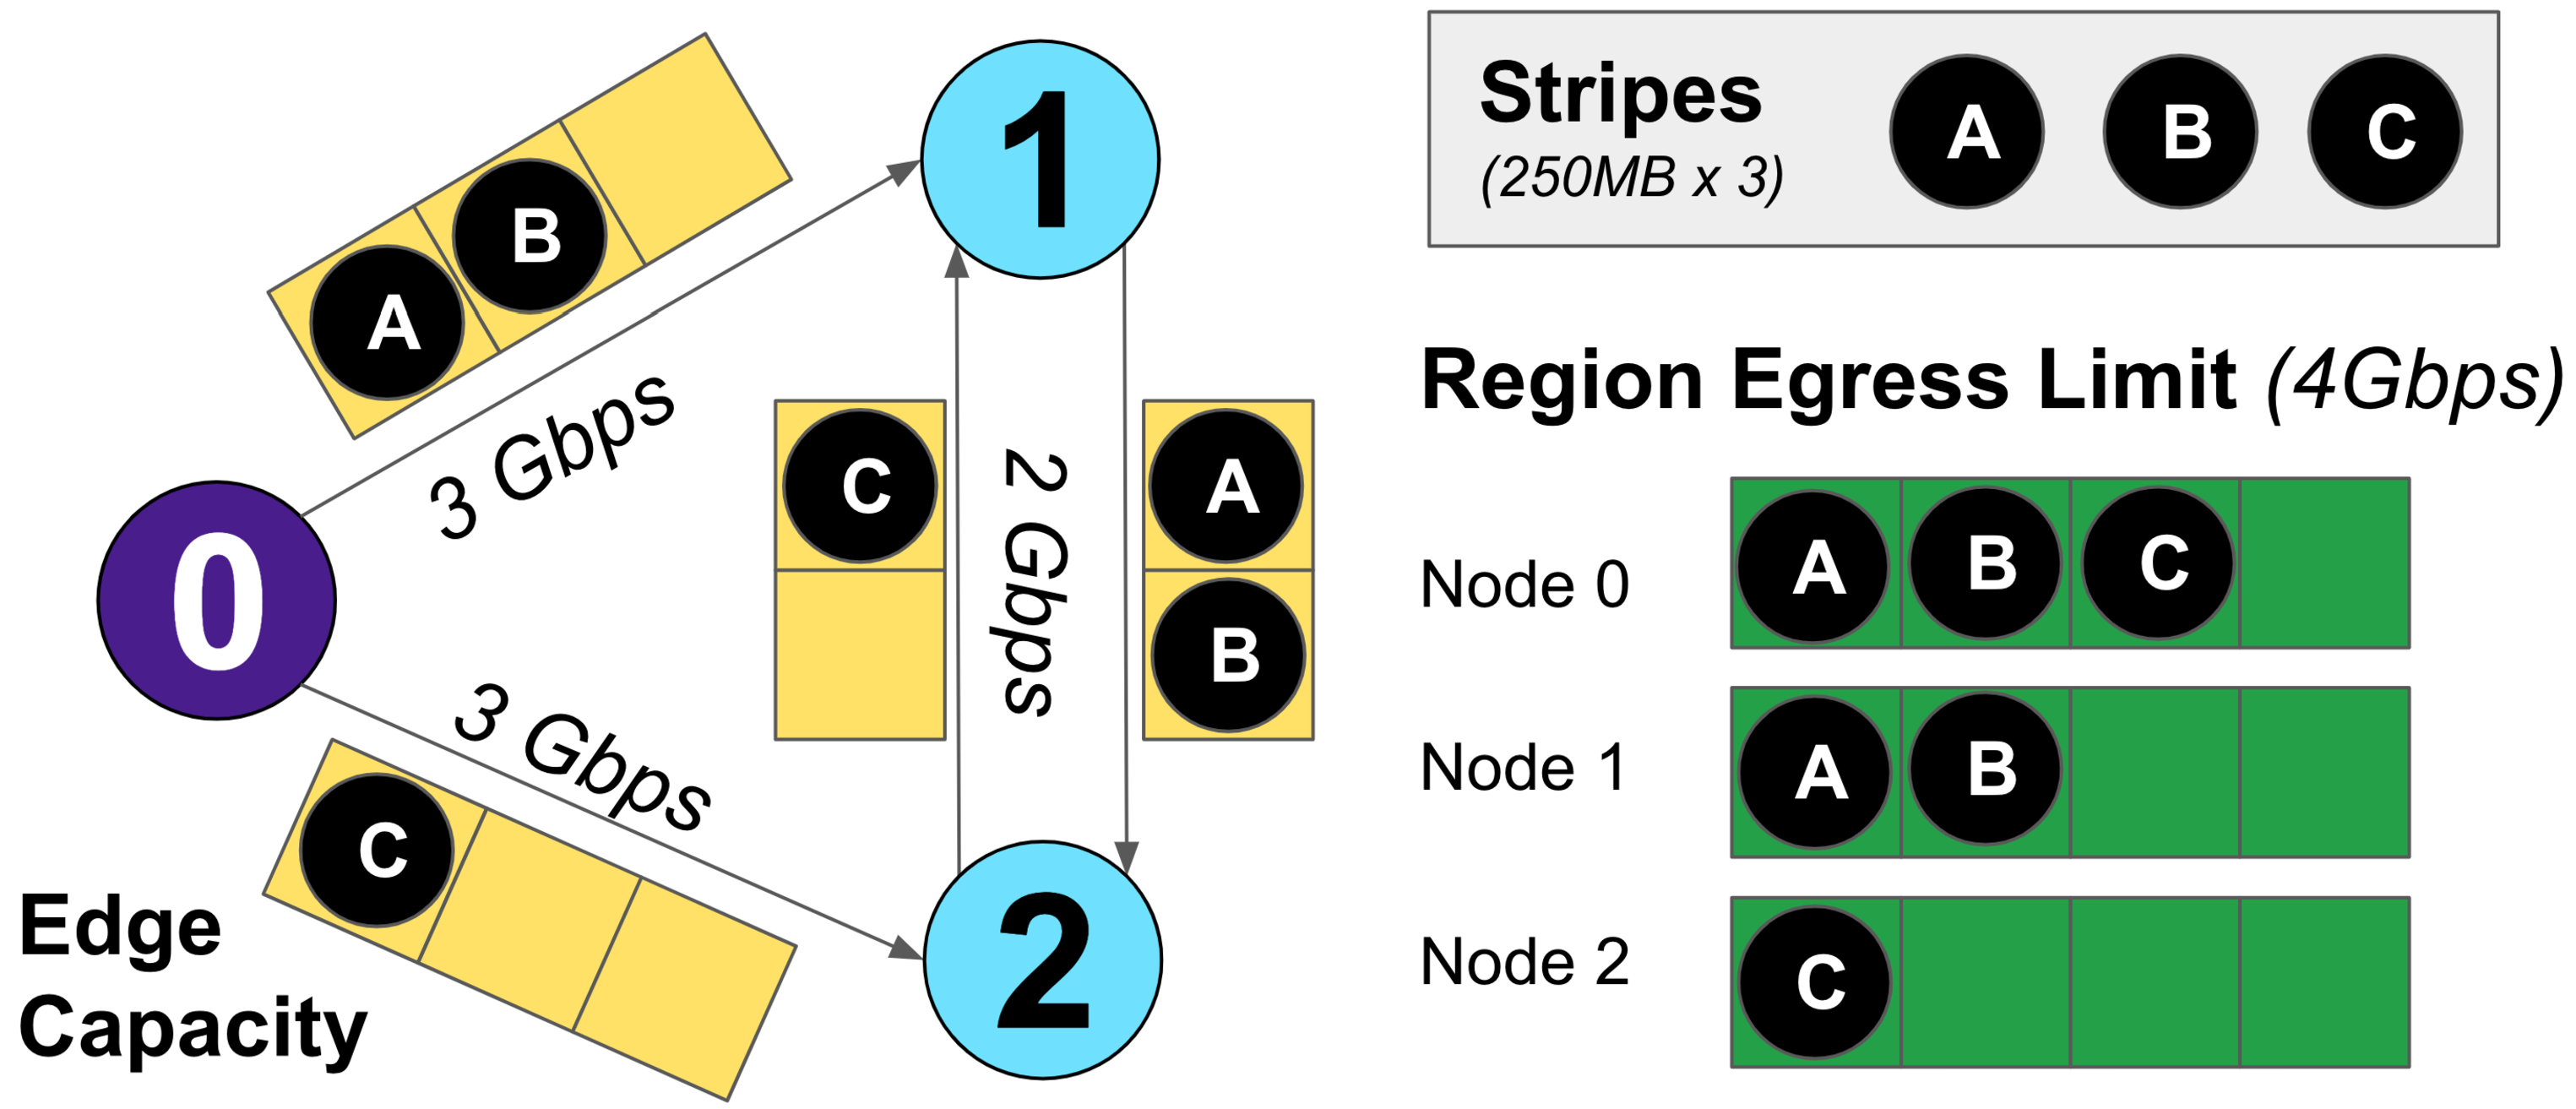
\includegraphics[width=0.8\linewidth]{figures/solver_overview.pdf}
     \caption{Stripes transferred from the source (purple) to destinations (blue) are placed by the solver along edges depending on edge capacity (yellow) and node capacity (green).}
     \label{fig:solver}
\end{figure}

% In order to minimize replication price while still meeting the runtime requirements and cloud resource constraints, we frame a MILP on top of a directed graph that represents the entire cloud topology. The input to the optimizer is the transfer size: $\size$, the runtime budget: $\runtime$, and the number of stripes: $\stripes$, where each stripe is a partition of the data that is routed along the same path. 

% We formulate the MILP in terms of how \textit{stripes} of data are allocated across cross-region paths, rather than throughput. 
% %
% Previous formulations allocate throughput to different edges in the network \cite{castro2003splitstream, zhang2018bds, ganguly2005fast}, which determines the overall throughput and latency of the multicast replication. However, to account for cloud pricing, which is charged per GB, we need to compute the number of bytes transferred along each edge. This introduces a non-linearity in the throughput formulation, as volume of the data transferred is the throughput allocated to the edge multiplied by the replication runtime. 

% In order to formulate the optimization problem as a MILP, we model the optimization problem in terms of allocating \textit{volume} to edges rather than throughput, where the units of allocation are per stripe. We translate cross-region bandwidth and per-region egress/ingress limits into volume capacities,
In order to minimize replication price while meeting runtime requirements and cloud resource constraints, we frame a MILP on a directed graph representing the entire cloud topology. The input to the optimizer is the transfer size: $\size$, the runtime budget: $\runtime$, and the number of stripes: $\stripes$ to divide the data into.

%We formulate the MILP concerning \textit{stripes} of data allocation across cross-region paths, rather than throughput.
%
%Previous formulations allocate throughput to different network edges \cite{castro2003splitstream, zhang2018bds, ganguly2005fast}, determining the overall throughput and latency of multicast replication. However, to account for cloud pricing, charged per GB, we need to compute the number of bytes transferred along each edge. This introduces non-linearity in the throughput formulation, as the data transfer volume is the throughput allocated to the edge multiplied by the replication runtime. 

To formulate the optimization problem as a MILP, formulate the problem in terms of allocating data \textit{volume} to edges rather than bandwidth, with allocation units per stripe. We translate cross-region bandwidth and per-region egress/ingress limits into volume capacities, as shown in \cref{fig:solver}, this determines how many stripes can fit along each edge. This makes the MILP similar to a bin packing problem, where we aim to pack stripes into edges such that all destinations receive all stripes. 
The volume-based representation allows cost to be computed as a function of the number of stripes placed on each edge. 

Next, we formally describe the MILP decision variables, objectives, and constraints. The cloud regions and cross-region paths are represented as $G=(V, E)$, where $V$ denotes the set of cloud regions and $E$ denotes paths between regions. We provide a reference table for the notation in \cref{tab:symbols}.

% as shown in Figure \ref{fig:solver}, which determines how many stripes can fit along each edge. This makes the MILP similar to a bin packing problem, where we want to pack stripes into edges such that all stripes are received by all destinations. 
% Furthermore, computing the cost is simplified by a volume-based representation since we can compute the egress cost from the number of stripes placed on each edge. 

% Next, we formally describe the MILP decision variables, objectives, and constraints. The cloud regions and cross-region paths are represented as $G=(V, E)$, where $V$ denotes the set of cloud regions and $E$ denotes paths between regions. We provide a reference table for the notation in \cref{tab:symbols}.

\subsubsection{Decision variables}

The MILP formulation consists of three decision variables. The path indicator variable $\indicator_{s, (v, u)}$ indicates whether a stripe $s$ is sent between regions $(u, v) \in V$. The paths selected by $\indicator$ make up the multicast replication tree for each stripe. The decision variable $\instances_v$ represents the total number of overlay routers in the region $v$. An additional flow variable $\flow_{s, (u,v)}$ ensures valid paths when constructing the multicast tree. 
It ensures that the paths selected by $\indicator$ do not contain cycles and are connected, by allowing flow to be pushed from the source to all destinations for each stripe (see \cref{constraints}).

\subsubsection{Objective: minimizing price under a deadline} \label{reduce_optimizer_runtime}

To minimize the price of a multicast transfer while meeting replication time constraints, we use a two-part objective function. The first part optimizes the number of virtual machines (VMs) per region, represented by $\instances$, and the second part optimizes the distribution trees per stripe, represented by $\indicator$. The objective is formulated as follows:
%
\begin{eqnarray}
    & \argmin_{\indicator,\instances}&  \underbrace{\runtime \times \frob{\costi} \instances}_\text{Instance Cost}  \\ 
    &+& \underbrace{\frac{\size}{\stripes} \times \sum_{s\in{\stripes}}  \frob{\coste} {\indicator_s}}_\text{Egress Cost}
\end{eqnarray}
%
The price of a data transfer is the sum of the instance fee and the egress fee. The instance fee depends on the number of VMs running per region, the job completion time, and the per-region VM fee. The egress fees are determined by the data distribution path and the amount of data traversed through the path, as defined by $\indicator$. We note that the instance cost is also an upper bound as it can be potentially overestimated if the data transfer is completed in less than the user-defined time budget. However, this is necessary to ensure linearity.

\subsubsection{Constraints}
\label{constraints}
We represent cross-region bandwidth, node egress/ingress bandwidth, per-region VM limits, and replication tree structure requirements as constraints within the MILP.

\heading{Representing Inter-Region \& Inter-Cloud Bandwidth} 
Cross-region bandwidth is represented as the \textit{per-GB capacity} given the run-time budget, i.e., how many stripes can fit along an edge. Increasing the number of VMs in the source regions linearly increases the rate at which we can send data. We thus model the bandwidth between two regions as the per-VM bandwidth profiled between those two regions multiplied by the number of VMs in the source region:
% As such, the volume capacity between the two regions is:
% \vspace{-0.1em}
\begin{equation}
    \capacitye = \frob{\instances} \bw * \runtime, 
\end{equation}
% \vspace{-0.1em}
and constrain $\indicator$ in terms of the path capacity: 
% \vspace{-0.1em}
\begin{flalign}
\forall (u, v)\in E 
    && \stripesize * \sum_{s} P_{s,(u,v)} \le \capacitye_{(u, v)}.
\end{flalign}
to ensure allocated stripes fit within the capacity. 

\heading{Representing VM Bandwidth Constraints}
Cloud providers impose per-VM bandwidth constraints on network egress, as described in \cref{ss:bandwidth-variability}. As such, a major bottleneck of multicast transfer is the source region's limited egress bandwidth. 
% 
We constrain $\indicator$ in terms of the ingress and egress limits: 
\begin{flalign} 
 \forall v \in V   &~~ \stripesize * \sum_{s}\sum_{u\in V} P_{s, (v, u)} \\ & ~~~~\le \capacityiegress_v * \instances_v * \runtime \\ 
\forall u \in V &~~ \stripesize * \sum_{s}\sum_{v\in V} P_{s, (v, u)} 
\\ & ~~~~\le \capacityiingress_u * \instances_u * \runtime 
\end{flalign}

\topheading{Representing VM Capacity Constraints}
We account for per region VM limits by adding the constraint $\instances \le \maxinstances$.

% Cloud providers limit the number of VMs that can be created per region, which we account for by adding a constraint $\instances \le \maxinstances$.\

\heading{Ensuring Valid Multicast Trees}
We use an additional variable $\flow$ to ensure that the paths selected by $\indicator$ are valid distribution trees, i.e., they are connected and acyclic, and they deliver all data to each destination. At a high level, we ensure that $\flow_{s, (u, v)}  \ge 1, \text{ if } \indicator_{s,(u,v)} = 1$, and impose conservation of flow constraints on $\flow$ but not $\indicator$, since $\indicator$ is an indicator variable not a flow variable. We then ensure that flow can be pushed from the source node to destination nodes on $\flow$ for each stripe, which also ensures that flow can be pushed from the source to destination for the paths selected by $\indicator$ (without having to impose flow conservation on $\indicator$). We leave details on this part of the formulation for \cref{s:formulation-details} due to space. 

\subsubsection{Solver feasibility}
Our formulation so far has a search space of size $O(2^{|V|^2\times|\stripes|})$. With 71 possible regions across GCP, AWS, and Azure and 10 stripes, the search space is, therefore, $O(2^{50410})$, which is infeasible even for advanced solvers to solve within a few minutes, necessitating approximations. 


% \subsection{ILP Formulation}


% We define a  problem for a set of equally sized partitions over a graph with known throughput and cost parameters over edges: 
% \begin{itemize}
%     \item $C$ = set of partitions (each of equal size $PARTITION\_SIZE$)
%     \item $V$ = vertices in the graph (i.e. regions). 
%     \item $COST_{edge}$ = $|V|\times|V|$, cost per GB of each edge
%     \item $TP_{edge}$ = $|V|\times|V|$, throughput of each edge
%     \item $COST_{instance}$ = $|V|$, cost per second running a VM in a region
% \end{itemize}
% There are three decision variables for the ILP: 
% \begin{itemize}
%     \item $P \in \mathbb{B}^{|C|\times|V|\times|V| }$: A boolean array indicating whether an edge is used to transfer a partition
%     \item $N \in \mathbb{N}^{|V|}$: An integer array indicating the number of VMs per region
%     \item $F \in \mathbb{Z}^{|C|\times|V|\times(|V|+1) }$: An integer array to ensure that for each partition, flow can be pushed along the partition's from the source vertex to all destination vertices. 
% \end{itemize}

% \subsection{Cost minimization}
% We define the objective as cost minimization as shown below: 
% \begin{equation}
%     \min \sum_{c \in C} P_c \times COST_{edge} \cdot PARTITION\_SIZE + N \times COST_{instance} \times s
% \end{equation}
% Given a deadline $s$, our optimization problem can be formulated as follows 
% \begin{gather}
% 	\underset{path, INST}{\text{arg min}}  \sum_{(u,v) \in E} \sum_{k=1}^{n} path_{(u,v),k} * \frac{VOLUME}{n} * COST_{(u,v)} + \sum_{i \in V} INST_i * \text{COST\_INS}_i * s \\
% 	\text {Subject to } \forall t \in D \text{, } \forall k \in \{1,...,n\} \sum_{(u,t) \in E}  path_{(u,v),k} \geq 1 \\
% 	\forall k \in \{1,...,n\} \sum_{(s,v) \in E}  path_{(s,v),k} \geq 1 \\ 
% 	\forall v \in V - \{s\} \text{ ,  }\forall k \in \{1,...,n\} \sum_{(v, w) \in E} path_{(v,w),k} \sum_{(u,v) \in E} path_{(u,v),k}  \geq \sum_{(v, w) \in E} path_{(v,w),k} \\ 
% 	\forall (u,v) \in E \sum_{k=1}^{n} path_{(u,v),k} * \frac{VOLUME}{n} \leq BW_{(u,v)} * s\\ 
%     \forall v \in V \sum_{(u,v) \in E} \sum_{k=1}^{n} path_{(u,v),k} * \frac{VOLUME}{n} \leq \text{vm\_ingress\_lim} * INST_v * s\\ 
%     \forall u \in V \sum_{(u,v) \in E} \sum_{k=1}^{n} path_{(u,v),k} * \frac{VOLUME}{n} \leq \text{vm\_egress\_lim} * INST_u * s
% \end{gather}

\subsection{Reducing Optimizer Runtime}
\label{ss:approximations}

In this section, we describe several mechanisms that we combine to reduce the optimization runtime or an order of seconds, while still maintaining solution quality. 

% \subsubsection{Stripe-Iterative Approximation}
% \vincent{a section with only 1 subsubsection is weird.  Just make everything a paragraph heading?} \shu{add}

\begin{figure}[tbp]
     \centering
     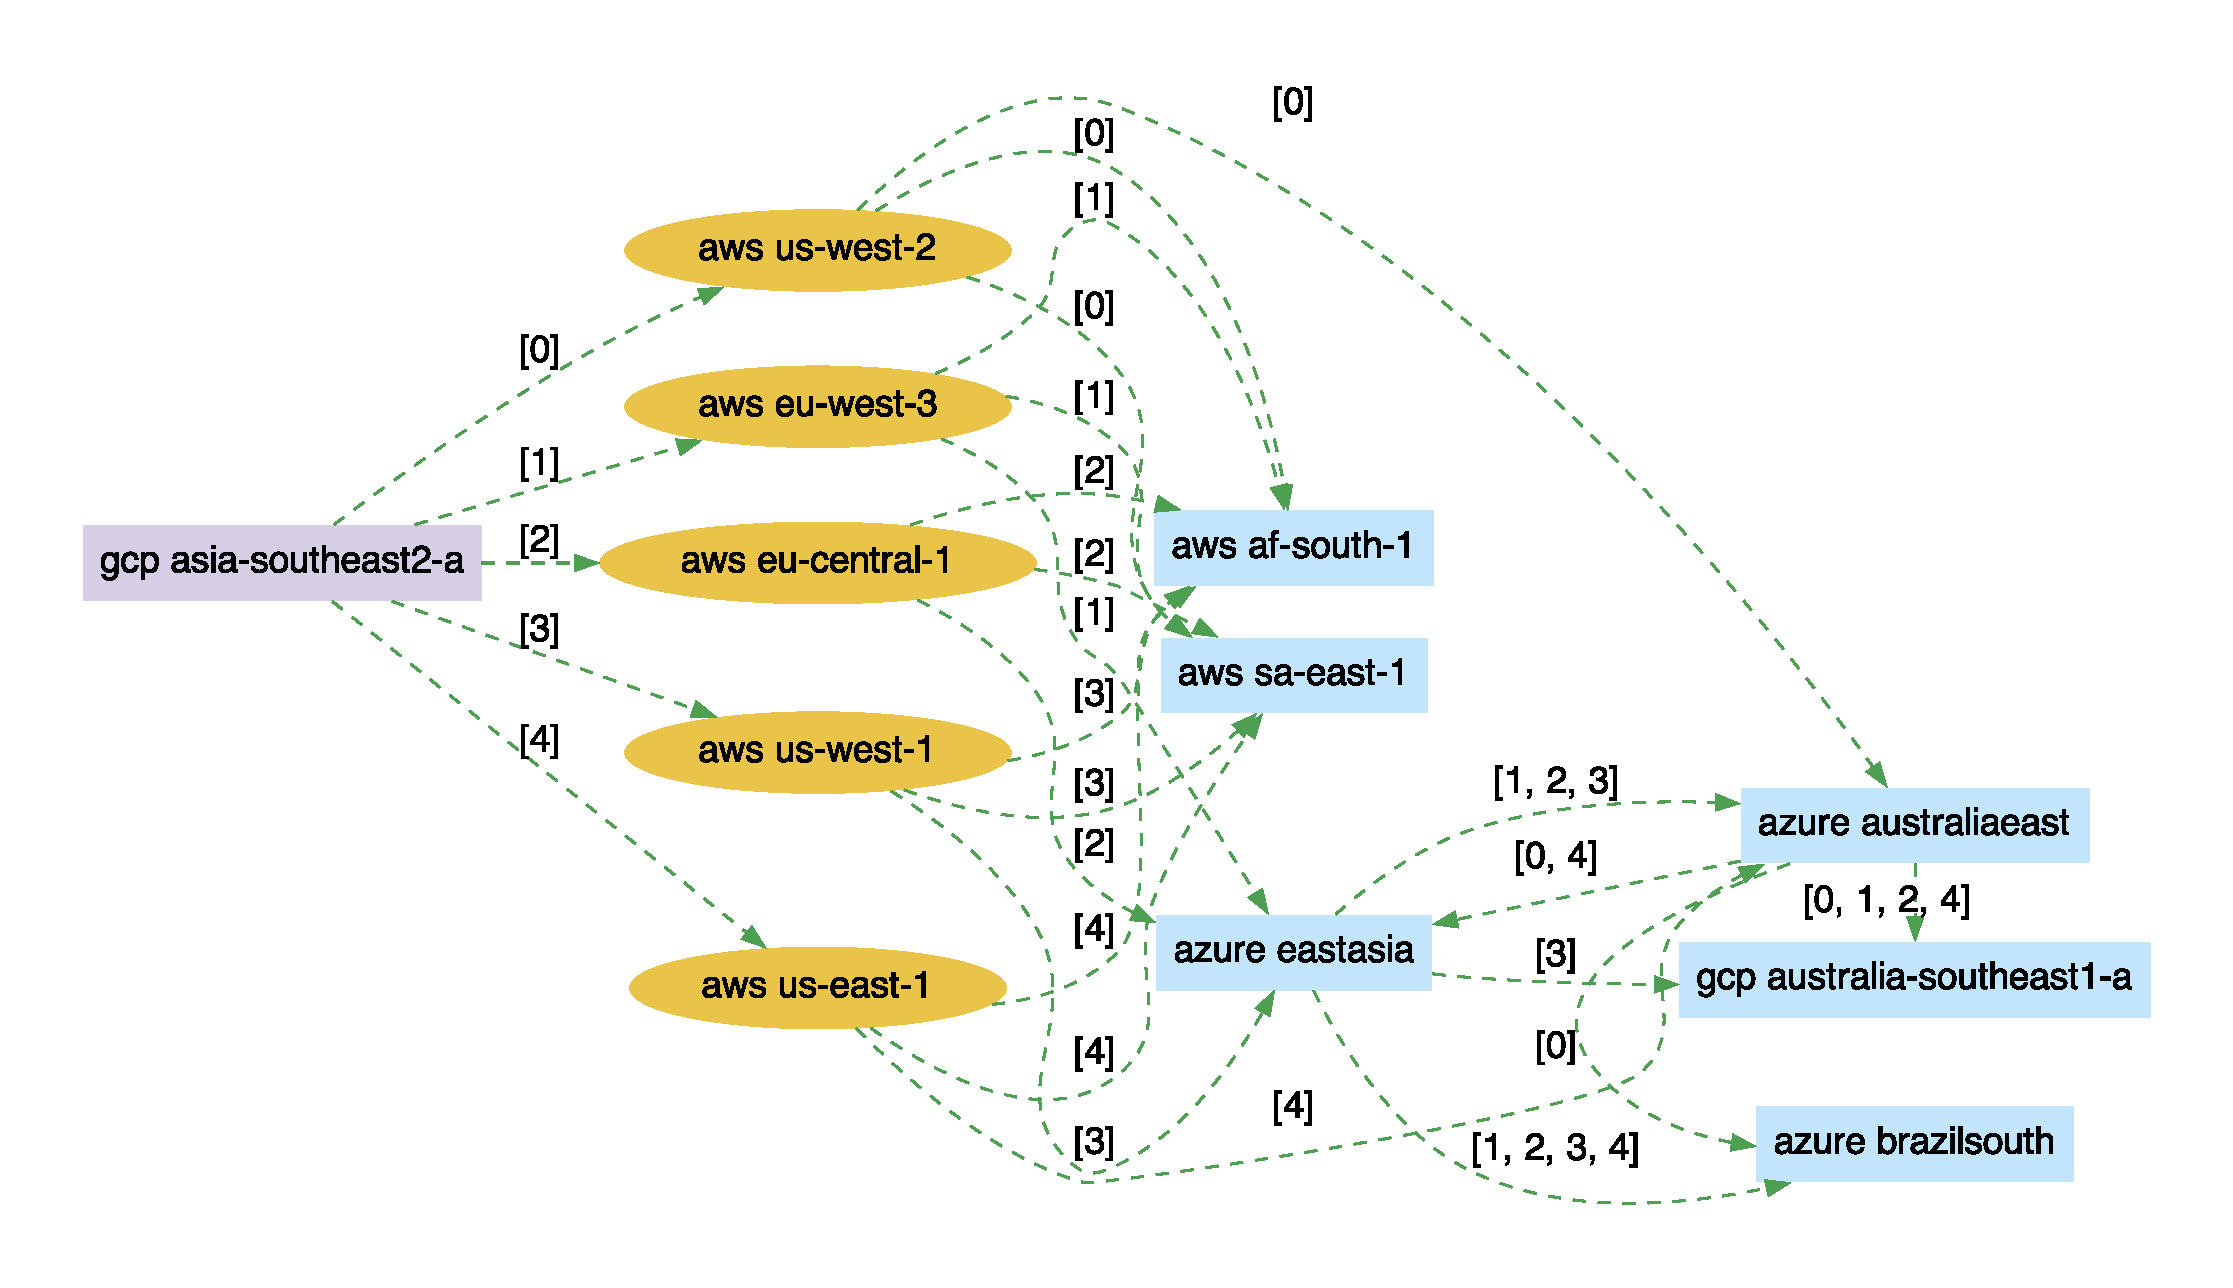
\includegraphics[width=\linewidth]{figures/partitions.pdf}
     \caption{Visualized solver output for inter-cloud replication described in \cref{sec:algorithm_eval}, consisting of source (purple), waypoint (yellow), and destination (blue) regions. The data is divided into 5 stripes (marked on edges). }
     \label{fig:example-topo}
\end{figure}

\heading{Node Clustering}
\label{node-filtering}
We observe that many regions across cloud providers share similar characteristics in terms of bandwidth and the costs of their outgoing and incoming paths. A motivating observation was that sub-sampling regions randomly could produce similar solutions with much lower solve time, as shown in Figure \ref{fig:node_selection}. At a high level, AWS regions in Europe regions all have similar egress/ingress costs and bandwidth, so only one of those regions needs to be considered as a potential waypoint. Therefore, to reduce the optimizer search space, we cluster regions using their incoming and outgoing path costs and bandwidth as features and select a representative node from each cluster. We empirically find that, with about 20 clusters (i.e. 20 subsampled regions), the optimizer can generate solutions that are reliably similar to the original MILP without approximation (more discussion in \cref{sss:solution_qual_eval}). 

%We aim to reduce the problem size and solve time by filtering out regions that may not be helpful in improving the solution quality. Our evaluation in \cref{fig:node_selection} shows that there is a diminishing return of solver solution quality with an increasing number of considered regions. Therefore, we implement node filtering by forming clusters of regions based on their profiled characteristics (e.g., cost, bandwidth) to all other available regions.

%By forming 20 clusters on 71 regions, we can speed up the solving time by a significant margin while maintaining solution quality within a reasonable range from the optimal solution. We select our set of considered regions by sub-sampling a single region from each cluster. Although node filtering carries the risk of reducing optimizer quality by leaving out potentially useful waypoint regions, we observe that there are sets of regions that contribute similarly to solving the multicast data replication tree. For instance, regions in similar geographic locations (e.g., Asia, or North America) might share similar characteristics, and only a small subset of them will be used by the MILP.
% We find out that in practice, forming 20 clusters on 71 regions speed up the solving time by \todo{xx} while still maintaining solution quality within xx\% from the optimal.

\heading{Hop Constraining}
\label{edge-filtering}
To further reduce the optimization space, we only consider a maximum of 2-hop overlay waypoints. Previous research has shown that limited numbers of overlay hops are often sufficient \cite{andersen2001resilient, peter2014one, stoica2002internet}. Our analysis also found solutions using multiple overlay hops to be rare, suggesting that they need not be considered. We implement the hop constraints as an additional constraint on the MILP. 

\heading{Stripe-iterative Approximation} To make the optimizer runtime linear with respect to the number of stripes (rather than exponential), we design a greedy, stripe-iterative approximation algorithm that solves for one stripe per iteration. We solve for each stripe independently, then update the input graph for the next stripe by reducing the path capacity ($\capacitye$), instance limits, and egress/ingress limits per region ($\maxinstances$, $\capacityiegress$, and $\capacityiingress$).

\subsection{Example Topology}
We show an example of the optimizer's output replication tree topology visualized in Figure \ref{fig:example-topo}. Due to variability in cloud provider egress pricing and cross-region throughput, our optimizer often finds unexpected solutions, such as routing one stripe (marked \texttt{[3]}) from GCP to AWS, AWS to Azure, then back to GCP. Although questionable at first glance, we evaluate this same replication in Figure \ref{fig:inter-cloud-1} and demonstrate both cost and replication time improvements over baselines. 

\section{Architecture of \sys{}}

A key contribution of this work is the design and implementation of the \sys artifact, which provides a practical, performant, and extensible system for studying overlay multicast algorithms in cloud environments.
The \sys{} system simplifies the design and deployment of multicast overlays spanning cloud object stores.
%\sys{} is highly extensible and supports pluggable algorithms for determining the location and number of overlay nodes to be created as well as the paths along with data is replicated.  
We use it to implement and deploy the optimizer described in \cref{sec:optimization} and several baseline algorithms.



%\sarah{is it necessary to discuss the differences/extensions needed to be made to Skyplane?}




\begin{figure}[t]
    \centering
    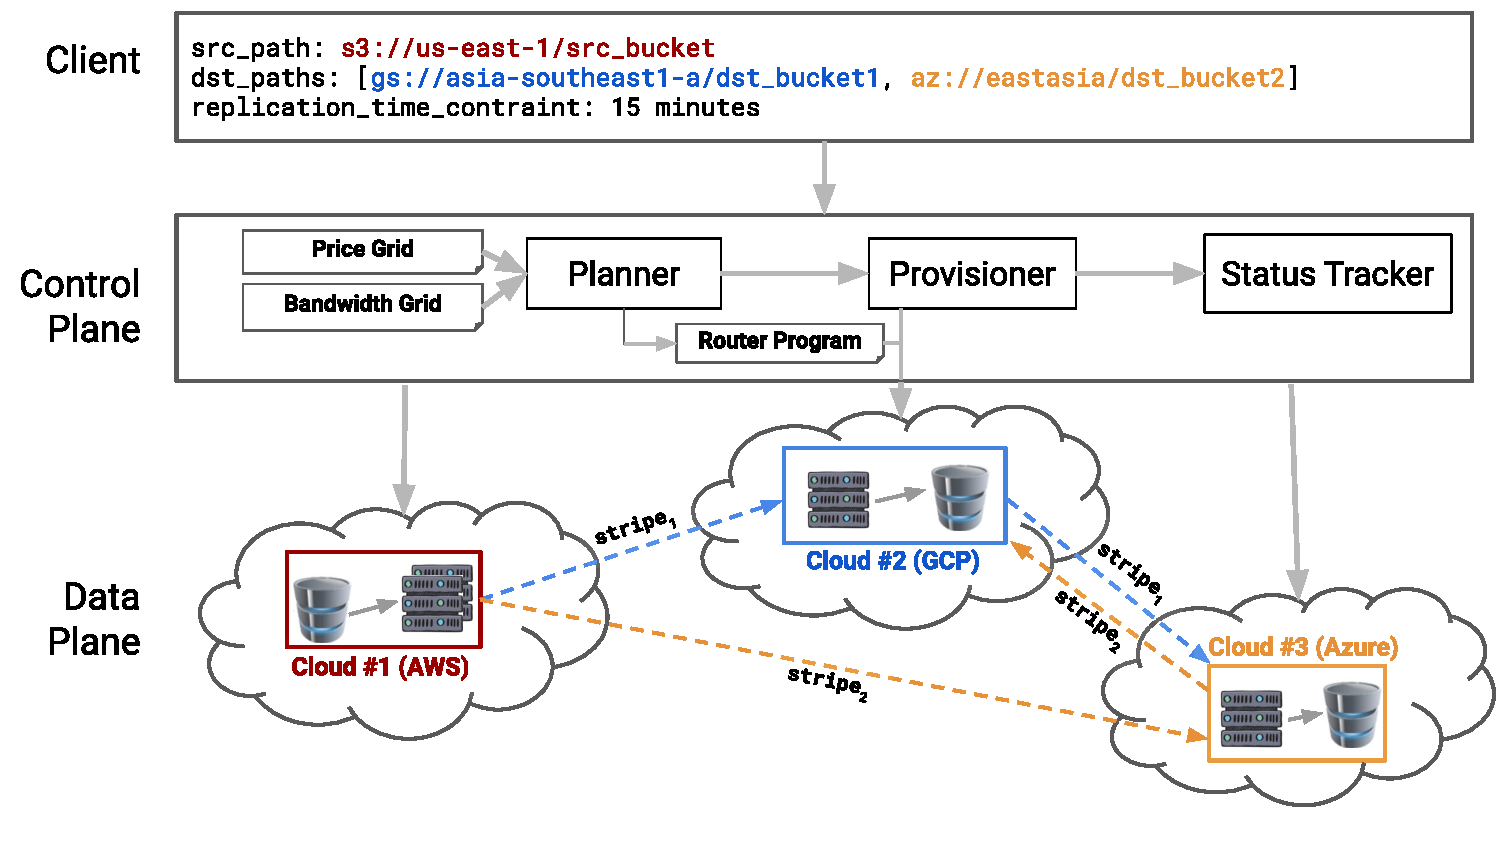
\includegraphics[width=\linewidth]{figures/cloudcast-architecture.pdf}
    % https://docs.google.com/presentation/d/1o04fk0svMe0Rg8bzGh-totPuRxAksQeNfPcIyaaWJgY/edit#slide=id.p
    \caption{\sys{} system architecture.}
    \label{fig:architecture}
\end{figure}




%To implement optimized multicast replication trees as well as baseline algorithms for real cloud replications, we develop \sys{}, a system for bulk data multicast between cloud object stores or VMs. \sys{} uses a user-provided target replication time and data path to determine a \textit{multicast plan} with the optimizer described in \cref{sec:optimization}, which identifies the location and number of overlay nodes to be created as well as how data should be replicated across the overlay. \sys{} then deploys cloud VMs to construct the overlay network and execute the replication as specified by the multicast plan. 


We provide an overview of \sys{} in \cref{fig:architecture}. \sys{} is designed with a centralized control plane and a distributed data plane. The control plane determines the set of overlay nodes and routing paths, and it dispatches and monitors multicast jobs. The data plane consists of \textit{overlay routers}, which we implement as modular software routers running on overlay nodes deployed on cloud VMs. \sarah{is this correct?} The control plane configures overlay routers using a \textit{router program}, which specifies a graph of modular operators for processing data.
Each overlay router gets a unique router program, which, in cooperation with other routers in the system, implements the desired flow of data over the overlay network.

\sys is implemented as part of the Skyplane \cite{jain2022skyplane} open source project and consisted of \todo{$\sim$18K} additional lines of Python to implement the \todo{overlay routers and XXX}.


\subsection{Control Plane}
%\sys{} uses a centralized control plane that can run on the client's machine or as a service in the cloud, and is responsible for initiating and monitoring replication.  
The control plane contains the planner, which supports pluggable algorithms for determining the placement of overlay routers across cloud providers and paths along which data is replicated (shown in \cref{fig:architecture}).
The output of the planner is used to provision VMs to act as overlay routers across cloud regions and to compile a router program for each overlay router that configures its behavior.
Finally, the control plane initiates the transfer and monitors its progress. 

\heading{Planner} 
The planner is responsible for creating a multicast plan based on a target replication time, source and destination object store paths provided by the user, and profiling data described in \cref{ss:profiling}.  
The planner takes as input the algorithm to use for generating a multicast plan, which can be the default \sys{} optimizer described in \cref{sec-optimizer} or a custom plan (e.g., a Steiner Tree over the cost graph). The planning algorithm determines how many overlay nodes to create in each region and how each data stripe should be routed through the overlay network. The planner uses the algorithm output to generate a \textit{router program} for each overlay router, which specifies how the overlay router should process a chunk header when received. 
The \sys{} default optimizer is implemented using Python's CVXPY library \cite{cvxpy} (version 1.3.2) with a Gurobi solver \cite{gurobi}, implemented in about $1$K lines of code.  

\heading{Provisioner} 
Once a multicast plan is determined, the provisioner instantiates the overlay routers.
The provisioner creates a VPC in each cloud provider and provisions VMs to act as overlay routers within these VPCs.
The provisioner also sets firewall rules to allow network traffic between overlay routers, which send and receive data from each other, as specified by the planner-generated router programs. 
Once a VM has been instantiated, the provisioner
installs and launches the router programs as containers on the VMs.

\heading{Chunk Dispatching and Status Tracker} 
The control plane subdivides replication target data into \textit{chunks}, which are at most 64MB in size, to allow for transfer pipelining and parallelism.
%Chunks are similar to packets but are larger to reduce metadata overhead.
Each chunk has a \textit{chunk header}, which specifies a key (e.g., object store object, filename), byte range, and an optional multipart ID (required for multipart uploads).
The chunk header also contains a \textit{stripe ID}, which specifies which path along the overlay the chunk will take. 

The control plane informs each source overlay router (i.e., overlay routers responsible for reading source data) the chunks for which they are responsible by sending the corresponding chunk headers.
We refer to this as \textit{registering} a chunk to an overlay router. 
%The control plane also uses cloud APIs to initiate multipart upload requests for large objects which are divided into multiple chunks. 
The control plane's status tracker monitors the status of each chunk by querying the status of chunks on each overlay router. 
%The controller maintains a status bar for transfer progress by monitoring chunk IDs marked as completed on the destination overlay routers (responsible for writing to the destination object store). 
%After all chunks have been completed processing, the controller finalizes the transfer by calling cloud provider APIs to mark any multipart upload requests are completed, and deprovisions the overlay routers. 
%These operations that directly interface with cloud API are separate from data plane operations.
% The status tracker also performs necessary logging and monitoring actions to ensure the transfer process is visible to end users. 

%\begin{comment}
%    \begin{lstlisting}[float=tp,basicstyle=\ttfamily\footnotesize,language=Python,caption={Example API call using the \sys{} solver.}, label={lst:api-example}]
%client = CloudcastClient()
%tracker = client.copy_async(
%    src="s3://source_bucket", 
%    dests=["s3://dest_bucket1", "gcp://dest_bucket2", "azure://dest_bucket3"], 
%    recursive=True, 
%    algorithm="cloudcast_opt",
%    replication_time_constraint_s=300
%)
%# monitor transfer status
%remaining_bytes = tracker.query_bytes_remaining()
%\end{lstlisting}
%\end{comment}


\subsection{Data Plane}
The data plane is composed of overlay routers, each running on a single VM. 
The overlay routers are created and configured by the control plane to execute the transfer according to the multicast plan. 
\sys{} supports configurable overlays by defining processing on overlay routers using modular operators, inspired by the design of configurable routers \cite{kohler2000click}.

The router program provided by the control plane specifies a directed acyclic graph (DAG) of \textit{operators} (analogous to elements) and \textit{connections}, all of which run on each overlay router and are used to process incoming chunk headers registered to the overlay router. \sarah{Should we just call them queues and operators, rather than using the click terminology?}
The DAGs are created at the overlay router's startup time based on the router program, and they allow overlay routers to process chunks without additional coordination with the control plane.

%elements are individual chunk processing modules, such as reading the chunk from the source object store, relaying the chunk to another overlay router's IP, or writing the chunk to a destination object store. Connections are queues that pass chunk headers between elements, and can be configured to send a chunk header to one or all of multiple downstream elements. 
%Each stripe ID corresponds to a unique DAG (so that different stripes can be routed differently). Chunk processing is pre-configured on each overlay router by the router program, and does not require any additional coordination with the control plane to decide how to process chunks.
%
%Each overlay router runs an HTTP server which receives chunk registrations (containing chunk header information), which the overlay router then processes via a DAG of \textit{elements} and \textit{connections}. 

\begin{table*}[t!]
\centering
\footnotesize
\renewcommand{\arraystretch}{1.1}
\begin{tabularx}{\textwidth}{ l X }
\toprule
    \textbf{System} & \textbf{Description} \\
    \midrule
    Direct & Data is transferred directly from the source to the destination regions.  \\
    MDST & Data is transferred along edges selected by a Minimum Directed Spanning Tree (including source and destination regions) computed from network costs. \\
    Steiner Tree & Data is transferred along edges selected by a Steiner tree (including optional waypoint regions) computed from network costs. \\
    SPIDER~\cite{ganguly2005fast} & Data is transferred according to the plan generated by SPIDER, a system designed for fast bulk replication to multiple destinations.\\
    Skyplane & Skyplane's optimizer is used to select paths for each source-destination pair, which are combined to build the distribution tree.  \\
    CloudMPCast~\cite{garcia2015cost} & Data is transferred over a set of cost-minimizing edges that meet a minimum bandwidth threshold. \\
    %\makecell[tl]{Cost-aware\\ Inter-DC Multicast~\cite{fatemipour2022cost}} & Data is transferred according to a solver that models cost and deadlines in the inter-DC context (e.g., bandwidth and switch-based pricing) according to \cite{fatemipour2022cost}. \\
    \makecell[tl]{Deadline-aware\\ Inter-DC Multicast~\cite{deadline2018}} & Data is transferred to meet deadlines in the inter-DC context according to \cite{deadline2018}. Note that due to scalability issues, we needed to modify the candidate tree generation step to only consider a subset of waypoint regions to achieve tractable runtimes. \\
    \makecell[tl]{AWS S3 Multi-\\Region Bucket~\cite{aws-replication}} & Vendor product that supports intra-cloud between AWS regions only. We enable Replication Time Control~\cite{aws-replication-time-control}.\\
    Bullet~\cite{kostic2003bullet} &  Data is transferred according to the plan generated by Bullet, a high-bandwidth dissemination technique using an overlay mesh.\\
    BitTorrent~\cite{twitter-bittorrent} & Peer-to-peer protocol where peers download data from each other in a decentralized manner.\\
    \midrule
    Cloudcast-Opt (HT) & Data is transferred along the highest throughput (HT) multicast tree generated by our optimizer (tightest time constraint).\\
    Cloudcast-Opt (LC) & Data is transferred along a low cost (LC) multicast tree generated by our optimizer (relatively loose time constraint).\\
    \bottomrule
\end{tabularx}
\caption{All of the systems and variants we evaluate, covering a mix of academic baselines and commercial solutions.}
\label{tab:baselines}
\end{table*}

Operators are implemented as a pool of worker processes running processing steps for a chunk, such as reading the chunk from the source object store, relaying the chunk to another overlay router, writing the chunk to a destination object store, or transforming the chunk data (e.g., compression or encryption).  Connections pass chunk headers between operators via thread-safe queues, and can be configured to send a chunk header to one or all of multiple downstream operators. 
%Although not used in our evaluation, by default, the object store download element is followed by elements to compress (via LZ4) and encrypt (\textcolor{red}{(todo:cite)})  chunk data; similarly, the object store upload is preceded by decompression and decryption. 
%New transformations to chunks (e.g. a different compression function) can be added by modifying the router program in the control plane. 
%The first element in the DAG must retrieve the data corresponding to some chunk header, either by downloading from the source object store or recieving data from another overlay router. 

For example, on a source overlay router, chunk registrations from the control plane will provide chunk headers to the first operator in the DAG, which downloads chunk data from an object store. All chunk data is stored in a shared memory filesystem to allow for fast access across operators. Once chunk data is downloaded, the chunk header is passed to the next operator via a connection, which runs LZ4 compression \cite{lz4}) and secret key encryption \cite{pynacl, libsodium} on the chunk data. The leaf operators are `sender' operators, which relay the chunk header and data to other overlay routers. 

%\heading{Relaying Chunk Between Overlay Routers} 
Chunk data is relayed between overlay routers by a `sender' operator on the sending router and a `receiver' operator on the receiving overlay router.
When the sender operator is created, it creates parallel TCP connections 
%(specified by the router program of the receiving overlay router), 
which are kept open for the duration of the transfer. 
Before sending chunk data, the sender will attempt to register the corresponding chunk headers with the receiving overlay router to ensure it has space in its shared memory file system to write the chunk data. Once chunks are registered, the sender will send the chunk data over the TCP sockets, and the receiver will wait for the written chunk data size to match the size specified by the chunk header, before sending chunk headers to the next operator. Successfully sent chunk data is deleted from the shared memory filesystem. 

\heading{Backpressure}  Connections are configured with a maximum size for the underlying queues. If the queue reaches its maximum size, the upstream operator will wait until the queue size decreases sending chunk headers to the connection.

\heading{Striping} Registered chunk headers with different stripe IDs are placed in different queues and processed by separate DAGs, so that different stripes can be routed differently.




%\subsection{Usage}

%\sys{} users can run multicast replication jobs using either a Python API or a CLI command.
%\sys{} requires that users authenticate with cloud provider CLI tools, which enable cached credentials to provision resources on the user's behalf to execute transfer requests.
%Listing~\ref{lst:api-example} shows an example of how a user specifies the source/destination paths and replication time constraints using the Python client. 

\section{Evaluation}

In this section, we evaluate \sys{} across three metrics: replication cost, replication time, and the optimizer solve time (or simply, runtime).
% 
In particular, we show that for intra-cloud and inter-cloud bulk data transfer, \sys{} is able to achieve up to 61.5\% cost improvements under a tight runtime budget when compared to academic, commercial, and open-source baselines.
% 
We also show that our approximations to reduce the optimizer solve time (as discussed in \cref{ss:approximations}) are highly effective by reducing the runtime by, on average, 30.68$\times$ for 5-destination replications. To simplify evaluation, we disable compression and encryption in experiments. 
%

%\subsection{Evaluated Systems and Algorithms} \label{sec:eval_baselines}
The full list of evaluated baselines is shown in \cref{tab:baselines}.
We note that many algorithms do not determine the number of VMs to use in each region.
To present them in the best light possible, we maximize the number of VMs in each region traversed by data, subject to per-region quota limits.



\if0
\begin{vitemize}
    \item \textbf{Direct}: Data is transferred directly from the source to the destination regions.  
    \item \textbf{MDST}: Data is transferred along edges selected by a Minimum Directed Spanning Tree (including source and destination regions) computed from network costs. 
    \item \textbf{Steiner Tree}: Data is transferred along edges selected by a Steiner tree (including optional waypoint regions) computed from network costs. 
    \item \textbf{SPIDER}~\cite{ganguly2005fast}: Data is transferred according to the plan generated by SPIDER, an academic baseline designed for fast bulk replication to multiple destinations.
    \item \textbf{CloudMPCast}~\cite{garcia2015cost}: Data is transferred along a set of cost-minimizing edges that meet a minimum bandwidth threshold. 
    %\item \textbf{Cost-aware Inter-DC Multicast}: Data is transferred according to a solver which models cost and deadlines in the inter-DC context (e.g. bandwidth and switch based pricing) as desribed by~\cite{fatemipour2022cost}. 
    \item \textbf{Deadline-aware Inter-DC Multicast}: Data is transferred to meet deadlines in the inter-DC context as described in~\cite{deadline2018}. 
    \item \textbf{AWS Multi-Region Bucket}~\cite{aws-replication}: Vendor product that supports intra-cloud between AWS regions only. We enable Replication Time Control~\cite{aws-replication-time-control}.
    \item \textbf{Bullet}~\cite{kostic2003bullet}: Data is transferred according to the plan generated by Bullet, a high bandwidth data dissemination technique using an overlay mesh.
    \item \textbf{BitTorrent}~\cite{twitter-bittorrent}: Peer-to-peer protocol where peers download data from each other in a decentralized manner.
    \item \textbf{Cloudcast-Opt (HT)}: Data is transferred along the highest throughput (HT) multicast tree generated by our optimizer given the tightest replication time constraint.
    \item \textbf{Cloudcast-Opt (LC)}: Data is transferred along the lowest cost (LC) multicast tree generated by our optimizer given a relatively loose replication time constraint.
\end{vitemize}
\fi

%Due to the large number of baseline algorithms and high cost of inter-cloud data transfer, we run comparisons across all academic baseline algorithms in simulation, and select the best performing baselines for end-to-end evaluation. 


% For transfers within a single cloud provider, we evaluate different academic baselines for generating multicast plans. 
% % 
% Each algorithm is implemented on top of \sys{}'s planner for consistency.
% % 
% We measure end-to-end replication time and the transfer cost.
% % 
% Many algorithms do not specify the number of VMs to use in each region, so we  maximize the number of VMs in each region which data traverses subject to per-region quota limits.
% % 
% % For example, if a waypoint region is selected by the Steiner tree, we create the maximum possible number of VMs in that region as our overlay routers.


\begin{figure}[t]
    \centering
    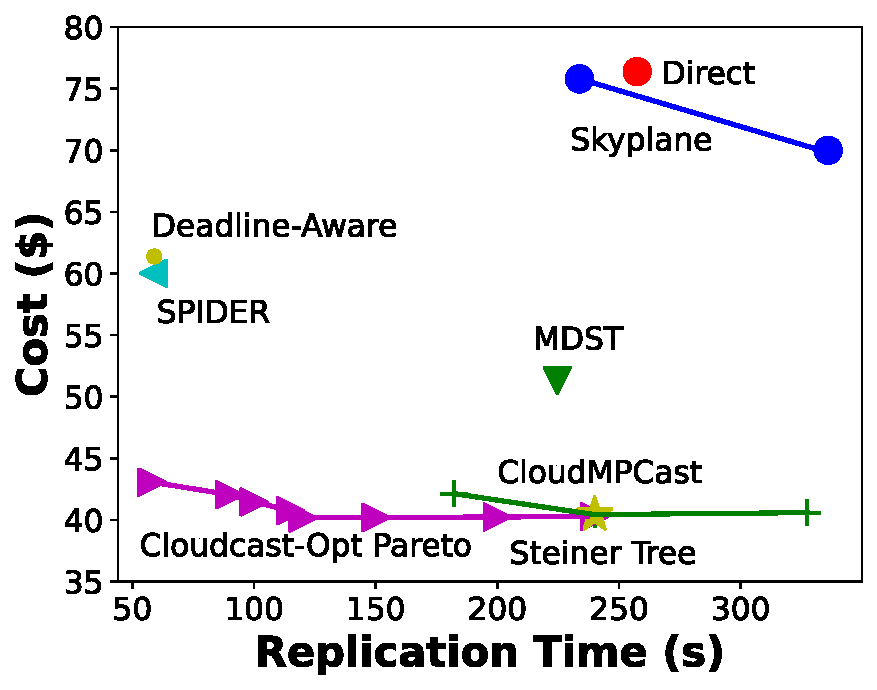
\includegraphics[width=
    0.35\textwidth]{figures/pareto.pdf}
    \caption{Simulated results for Multicast Algorithms.} 
    \label{fig:simulated-baselines}
\end{figure}

\begin{figure*}[tbp]
     \centering
     \begin{subfigure}[b]{0.33\textwidth}
        \centering
        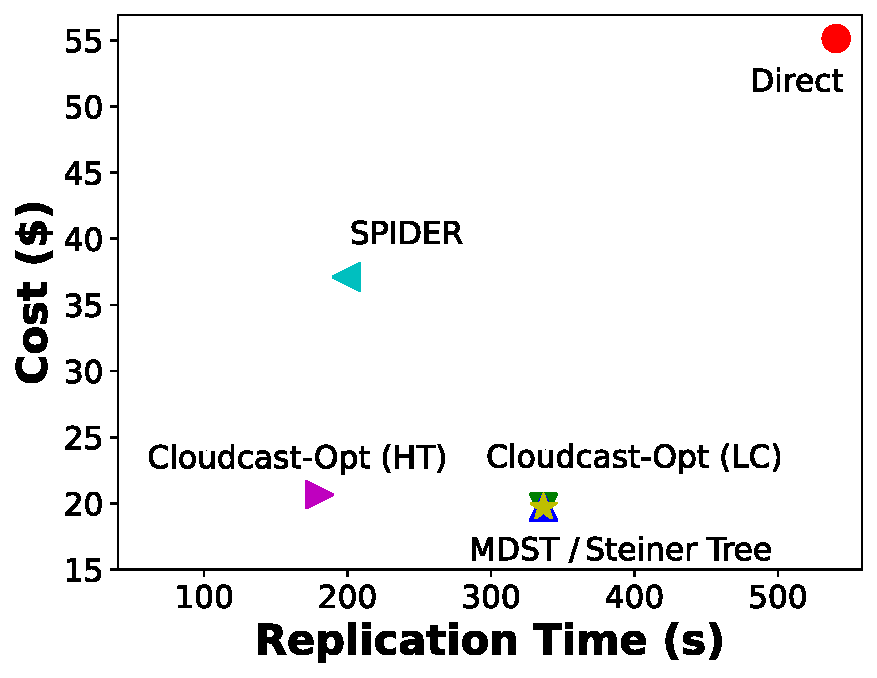
\includegraphics[width=\textwidth]{figures/aws.pdf}
        \caption{AWS Intra-Cloud}
        \label{fig:aws-intra-cloud}
    \end{subfigure}
    \hfill
    \begin{subfigure}[b]{0.33\textwidth}
        \centering
        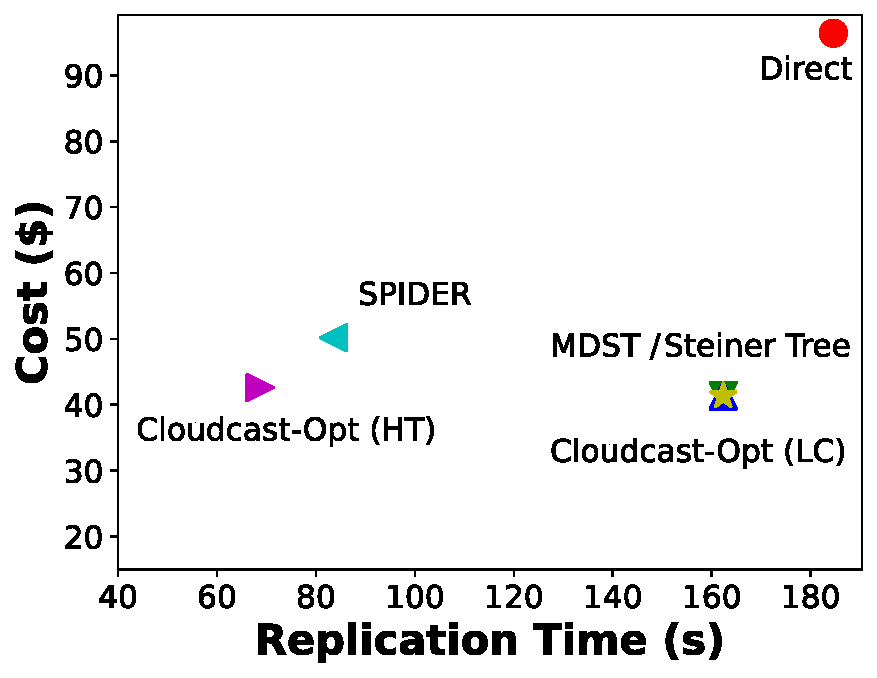
\includegraphics[width=\textwidth]{figures/azure.pdf}
        \caption{Azure Intra-Cloud}
        \label{fig:azure-intra-cloud}
    \end{subfigure}
    \hfill
    \begin{subfigure}[b]{0.33\textwidth}
        \centering
        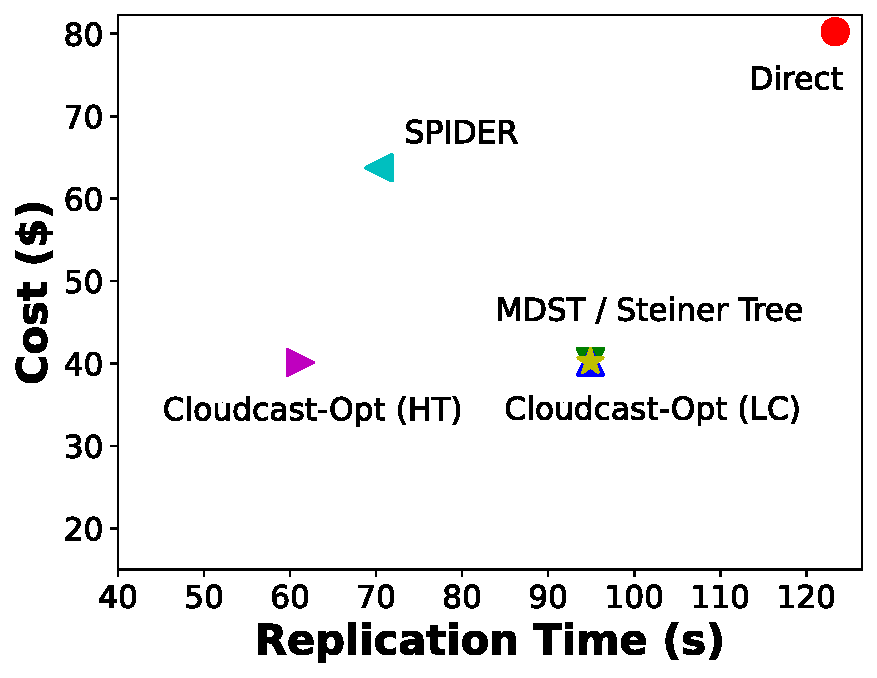
\includegraphics[width=\textwidth]{figures/gcp.pdf}
        \caption{GCP Intra-Cloud}
        \label{fig:gcp-intra-cloud}
    \end{subfigure}
    \hfill
    %\vspace{-2em}
    \caption{Intra-cloud multicast results for algorithms implemented on \sys{}.  
    %In all cases \sys{}-Opt is able to find significantly faster low-cost solutions where compared with existing techniques.  Furthermore, the MDST/Steiner Tree solution using ephemeral waypoints is able to consistently find the cost-optimal solution.  
    % \shu{we need to explain why we use these topologies, as well as why there are some variances in the running outcomes (e.g. SPIDER is closer to Cloudcast in Azure, or AWS runtime is much worse than the other cloud)}
    }
    \label{fig:intra-cloud}
\end{figure*}
\begin{figure}[tbp]
    \centering
    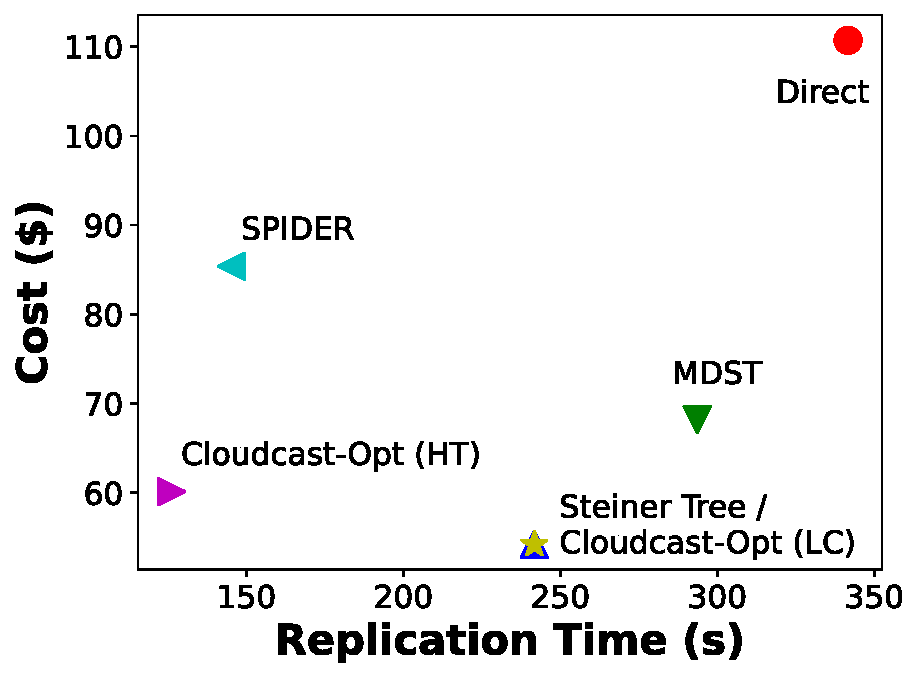
\includegraphics[width=
    0.33\textwidth]{figures/inter_cloud.pdf}
    \caption{Inter-cloud multicast results for different algorithms implemented on \sys{}. The \sys{} replication tree is visualized in Figure \ref{fig:example-topo}.
    % \joey{Figures should have a clear "takeaway" in the caption.  What would you say if presenting this figure in a talk.}
    }
    \label{fig:inter-cloud-1}
\end{figure}

\subsection{Comparison to Multicast Algorithms}
\label{sec:algorithm_eval}

% Using \sys{}, 
We compare the replication time and cost of existing multicast algorithms with \sys's optimizer to send 100\,GB of data from one source to six destination regions.

\heading{Simulation results}
Given the above replication scenario, we start by exploring a wide range of algorithmic baselines and \sys parameter settings through simulation.
While we tested many configurations through the development of \sys, due to limited space, we present results for a representative configuration\footnote{Simulated Inter-Cloud: from \path{gcp:asia-southeast1-a} to \path{azure:eastasia}, \path{aws:af-south-1}, \path{azure:brazilsouth}, \path{aws:sa-east-1}}.
Evaluated systems include \sys-Opt, direct transmission to the destinations, sending along cost-minimizing trees (MDST and Steiner Tree),  SPIDER~\cite{ganguly2005fast}, CloudMPCast~\cite{garcia2015cost}, Skyplane~\cite{jain2022skyplane}, and a deadline-aware inter-DC optimizer~\cite{deadline2018}.
Although Skyplane's optimizer is designed for unicast, not multicast, we adapt the optimizer's solution to multicast by running the optimization for each source-destination pair, and then combining all the graphs to build the distribution tree. 

For Skyplane, CloudMPCast, and \sys-Opt, we vary the throughput parameter to evaluate the performance range.  
For CloudMPCast~\cite{garcia2015cost}, the optimizer 
%it uses an optimizer that minimizes cloud egress costs by replicating data over min-cost Steiner Tree computed over edges with at least as much bandwidth as the the original source-destination path (to ensure minimal throughput degradation).
%CloudMPCast
allows for the level of throughput degradation to be controlled by an $\alpha \le 1$ term, which determines how aggressively edges are filtered out.
Our parameter sweep includes $\alpha \in [1, 0.5, 0.1]$, where $\alpha=1$ maximizes CloudMPCast's throughput.
For Skyplane, we vary the target throughput to maximize throughput and minimize cost, and plot both of these points. 
For \sys-Opt, we show results for several replication time constraints.

In \cref{fig:simulated-baselines}, we see that all baselines improve significantly upon direct transmission, and while some can match \sys-Opt's capacity for fast replication time or low cost, no existing baseline can optimize both metrics simultaneously.
Rather, \sys-Opt's Pareto-curve can match or beat all baselines on at least one of cost or performance.
CloudMPCast, whose $\alpha$ parameter does provide some flexibility, still offers a worse tradeoff than \sys-Opt.
Skyplane also has a significantly worse tradeoff curve, as it is not designed for multicast, so does not perform optimizations to alleviate source bottlenecks which are crucial for achieving high throughput. Despite this, even Skyplane's can improve throughput (for the throughput-maximizing solution) and reduce cost (for the cost-minimizing solution) as compared to direct transfers. 
%as CloudMPCast does not directly optimize throughput. VL: I didn't know what this meant

%\textcolor{red}{TODO: fix this text}
%We can observe that the Pareto-curve for CloudMPCast offers a worse tradeoff than \sys in \cref{fig:simulated-baselines}, as CloudMPCast does not optimize throughput. We also implement  \cite{luo2019deadline}, which combines multiple distribution trees similar to SPIDER and, as a result achieves similar cost and throughput results. 


%show additional algorithmic baselines in simulation, shown in \cref{fig:simulated-baselines}, where we also implement 

\heading{Cloud deployments}
The remainder of our evaluations present empirical results from real cloud data transfers.
Due to the high cost of running data multicast in the cloud (\$20--\$110 per transfer), we limit our evaluation to four representative configurations and four representative baselines identified by our simulation results.
Among the configurations, three are intra-cloud replications corresponding to AWS\footnote{AWS Intra-Cloud: from \path{ap-east-1} to \path{us-west-1}, \path{ap-northeast-3}, \path{eu-north-1}, \path{ap-south-1}, \path{ca-central-1}, \path{ap-northeast-1}}, Azure\footnote{Azure Intra-Cloud: from \path{brazilsouth} to \path{westeurope}, \path{westus}, \path{koreacentral}, \path{australiaeast}, \path{uaenorth}, \path{centralindia}} and GCP\footnote{GCP Intra-Cloud: from \path{asia-southeast2-a} to \path{australia-southeast1-a}, \path{southamerica-east1-a}, \path{europe-west4-a}, \path{europe-west6-a}, \path{asia-east1-a}, \path{europe-west2-a}}, and one is an inter-cloud replication workload that covers all three major providers\footnote{Inter-Cloud: from \path{gcp:asia-southeast1-a} to \path{azure:australiaeast}, \path{azure:eastasia}, \path{aws:ap-southeast-2}, \path{azure:brazilsouth}, \path{aws:sa-east-1}, \path{gcp:australia-southeast1-a}}.
These configurations are chosen to contain a source region with high egress costs to demonstrate potential cost savings.
Among the baselines, we sub-selected the best-performing baselines from our simulation results in terms of throughput (SPIDER) and cost (Steiner Tree), with direct transmission providing a naive baseline.

%, and demonstrate an ablation with randomly selected source and destination regions in Figure \ref{fig:dest_ablation2}.

\cref{fig:aws-intra-cloud,fig:azure-intra-cloud,fig:gcp-intra-cloud} show results for AWS, GCP, and Azure intra-cloud replication, and \cref{fig:inter-cloud-1} shows inter-cloud results.
Across all configurations, given a very tight replication time constraint, \sys{}-Opt (HT) solution leads to $46-62.4\%$ cost reductions and $2-2.84\times$ replication time speedup compared to sending directly to each destination. 

Of the baselines tested, SPIDER~\cite{ganguly2005fast} consistently demonstrates the lowest replication time, as it did in simulation.
However, as SPIDER is not cost-aware, \sys{}-Opt (HT) can achieve $28.4-44.0\%$ cost savings.
Surprisingly, while saving significant cost, \sys{}-Opt (HT) simultaneously speeds up replication by $1.11-1.35\times$, beating SPIDER on both axes.
%while still maintaining $1.11-1.35\times$ replication speedup compared to this algorithm. 
If, on the other hand, 
\sys is given a loose replication time budget, i.e., \sys{}-Opt (LC), it can find the cost-optimal solution in all setups, matching Steiner Tree solutions.

% \begin{figure}[tbp]
    \centering
    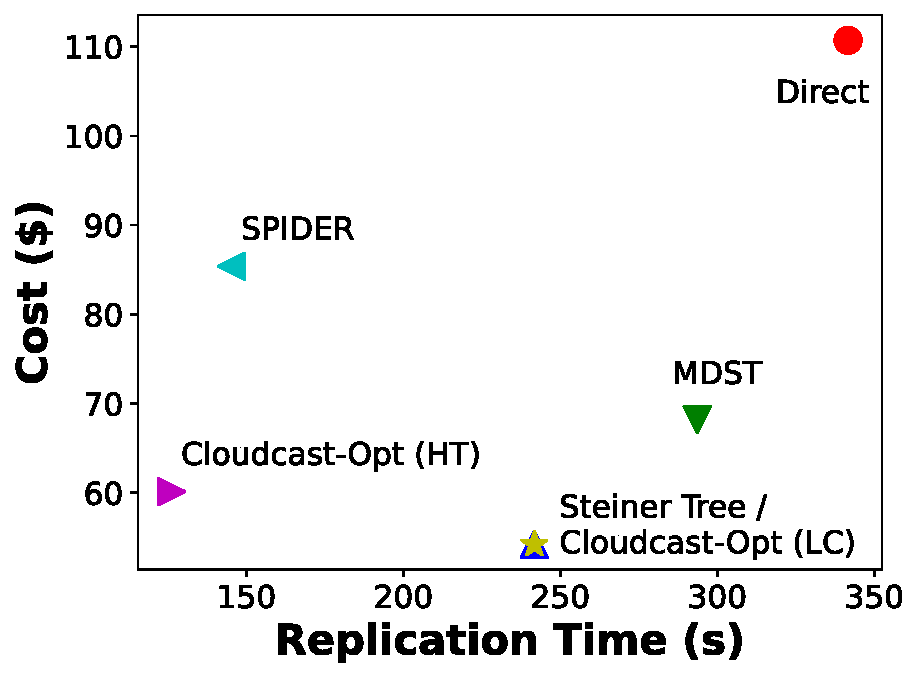
\includegraphics[width=
    0.33\textwidth]{figures/inter_cloud.pdf}
    \caption{Inter-cloud multicast results for different algorithms implemented on \sys{}. The \sys{} replication tree is visualized in Figure \ref{fig:example-topo}.
    % \joey{Figures should have a clear "takeaway" in the caption.  What would you say if presenting this figure in a talk.}
    }
    \label{fig:inter-cloud-1}
\end{figure}





%We run \sys{}-Opt with only two replication time budgets---tight and loose---but we note that \sys{}-Opt is able to find multiple points on the cost-replication time Pareto frontier, as shown in Figure \ref{fig:simulated-baselines}. 
%In fact, \sys{}-Opt can always generate an equivalent cost-minimizing multicast plan to the Steiner Tree, given a loose replication time budget.
%What distinguishes \sys{}-Opt from the Steiner Tree is the ability to trade off cost and replication and also to select the lowest replication time solution among cost-equivalent Steiner Trees. For example, for GCP and Azure intra-cloud transfer, \sys{}-Opt can identify a multicast replication tree of the same cost with $2.5\times$ and $1.6\times$ replication speedup compared to the Steiner Tree.



\subsection{Cloud Provider and P2P Systems}
\label{sec:sys_eval}
We run end-to-end evaluation comparing \sys{} with a commercial baseline (AWS S3 multi-region bucket replication) and P2P systems (BitTorrent and Bullet). 

\subsubsection{AWS S3 Multi-Region bucket replication}
We run an end-to-end comparison between \sys{} and AWS's S3 multi-region bucket replication\cite{aws-replication} for single-provider multicast.
AWS supports adding multiple replication rules to a source bucket to specify automatic replication to one or more replication buckets. 
% NOTE: below line added by Simon
%In comparison, GCP and Azure only support point-to-point transfers and do not provide a data replication product that supports multiple destinations. GCP's multi-region bucket \cite{gcp-multi-region-bucket} does not explicitly transfer to multiple destinations, and it is bounded by geographical regions. 
In the aspect of time control, AWS supports a replication time control with a minimum 15-minute SLO. However, we found that in our experiments, replications typically completed much faster than 15 minutes. Therefore, we use the actual replication time as a point of comparison. 

We compare AWS's replication time and cost to \sys{} with the planner implemented with both direct transfer and the optimizer. 
We transfer an OPT model~\cite{zhang2022opt} with 66 billion parameters ($122$\,GB in total across 9 files) between regions in a single continent\footnote{from \path{aws:ap-east-1} to \path{aws:ap-southeast-2}, \path{aws:ap-south-1}, \path{aws:ap-northeast-3}, \path{aws:ap-northeast-2}, \path{aws:ap-northeast-1}}.
To evaluate AWS replication time and cost, we create buckets with replication rules from a bucket in the source region to buckets in destination regions. 
Once the replication rules are created, we copy data from a bucket in the same region into the source bucket with 16 VMs. After the write completes, we measure the time until the completion of replication into all destination buckets. We calculate the transfer cost according to AWS's pricing page \cite{aws-data-transfer-cost}. We compare AWS multi-region bucket replication to \sys{} implemented with both the direct and optimizer planner and running.  As shown in Figure \ref{fig:aws_comparison}, the direct transfer has the same egress costs as AWS bucket replication, but the VM costs are much less than the service fee charged by AWS for the replication. Overall, \sys{} with the optimizer is able to achieve $2.3\times$ replication speedup and $61.5\%$ cost savings. This is a result of being able to leverage VM parallelism as well as an overlay network that minimizes total egress costs.  

\begin{figure}[t]
    \centering
    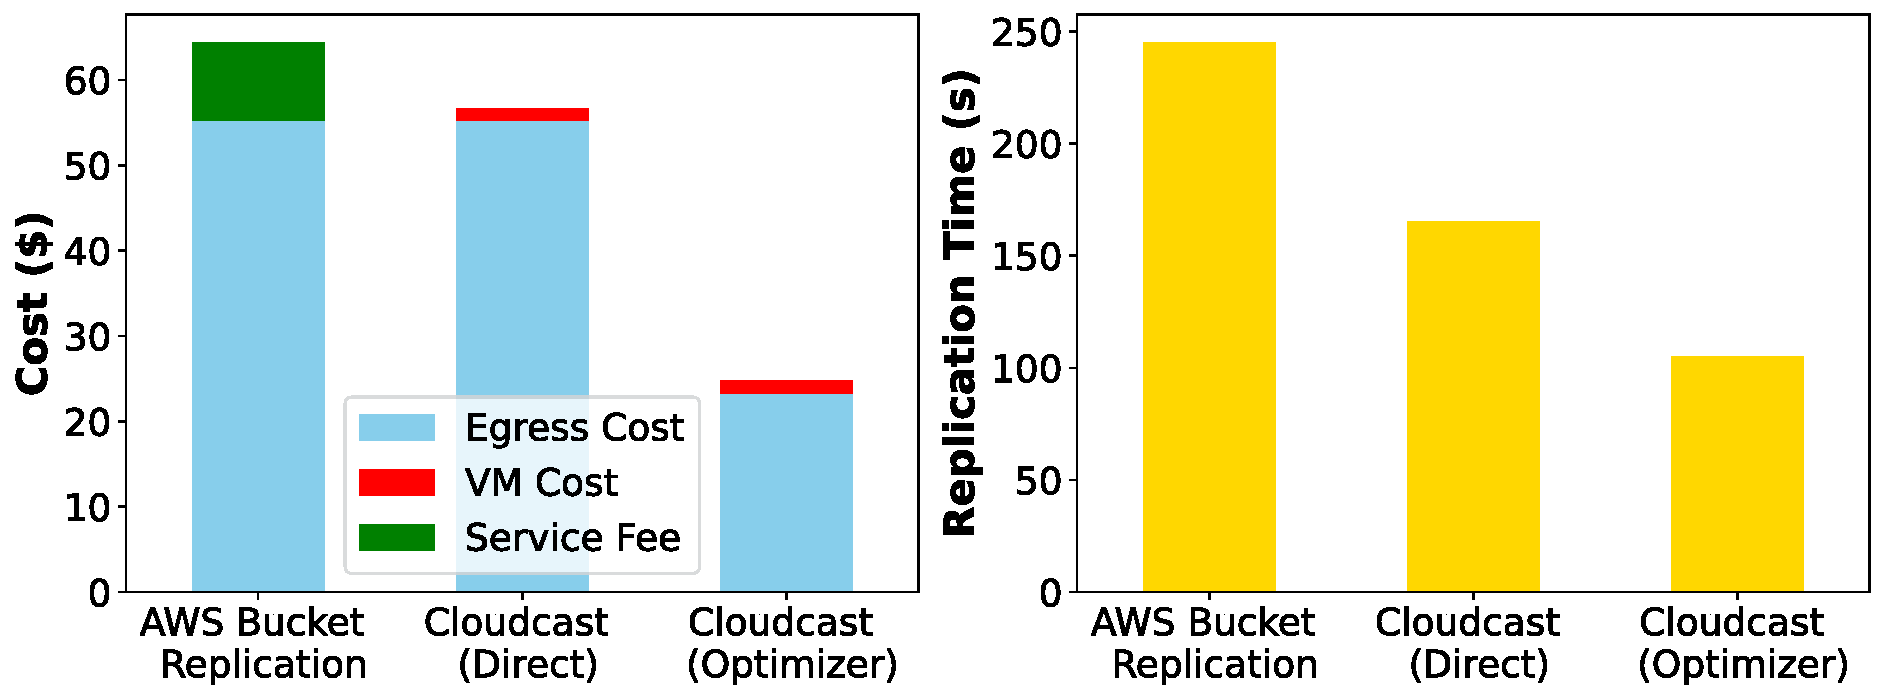
\includegraphics[width=
    \linewidth]{figures/opt_e2e.pdf}
    \caption{\sys{} outperforms AWS S3 Replication Time Control while reducing total transfer costs.} 
    \label{fig:aws_comparison}
\end{figure}

\subsubsection{P2P BitTorrent and Bullet}

We also compare \sys{} against P2P systems like BitTorrent and Bullet. 
%P2P systems are natural choices for transferring large files over multiple destinations. 
We run the same transfer benchmark in Azure in Figure \ref{fig:azure-intra-cloud}, sending 100GB within Azure to 6 destination regions. We host our own BitTorrent tracker and use aria2~\cite{aria2} as a BitTorrent client. Since Bullet's implementation is not available, we evaluate Bullet by implementing Bullet's algorithm inside \sys{}'s planner. The result is shown in Figure \ref{fig:p2p_comparison}: both BitTorrent and Bullet have lower egress costs than direct but higher than \sys{}. BitTorrent is the slowest because most clients cannot utilize the full bandwidth. The clients are built for scenarios like background seeding and transfer off the critical path, rather than for bulk data transfer. Interestingly, without a centralized planner, BitTorrent is able to find a low-cost multicast replication tree by inferring the bandwidth among peers and preferring the data from peers who have the highest throughput. However, it is still significantly more expensive than \sys{}. 
%Peers also communicate with each other by requesting "pieces" and sending "choke" signals. The end result is an all-to-all communication graph that preferred high bandwidth regions like US, Canada, and Europe. 

\begin{figure}[t]
    \centering
     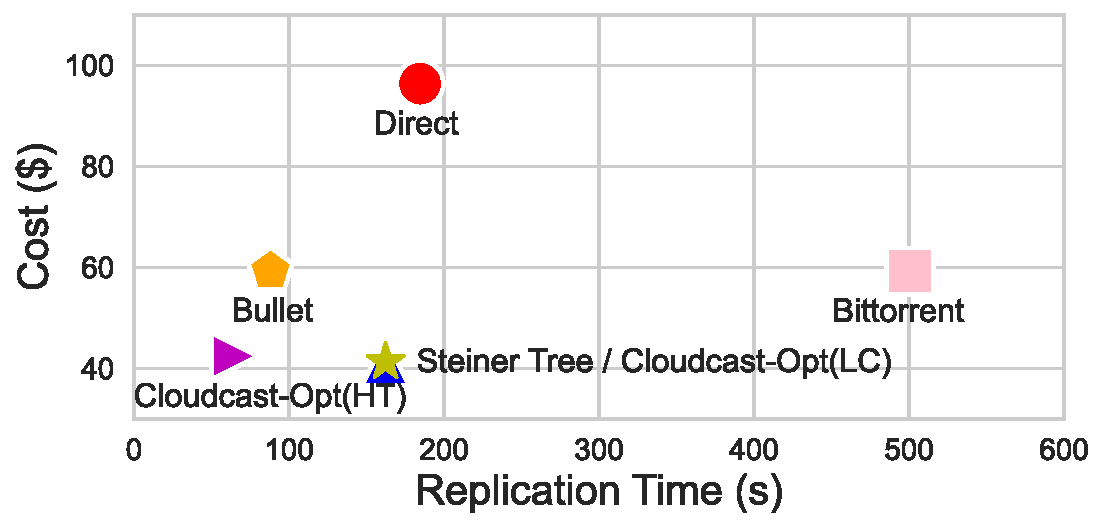
\includegraphics[width=.85\linewidth]{figures/p2p-comparison-all.pdf}
    \caption{Comparison with BitTorrent protocol on the intra-cloud Azure workload in Figure \ref{fig:azure-intra-cloud}. 
    %BitTorrent is cost-conserving as compared to direct transfer. It has the highest runtime because the BitTorrent clients are not designed to efficiently utilize the full available bandwidth.
    }
    \label{fig:p2p_comparison}
\end{figure}

\subsection{Ablations of \sys{}'s Optimizer}
\label{sec:simulated_section}
To understand how our optimizer behaves for different selections of source and destination regions and different target replication times, we run simulated ablations. 
%Due to the high cost of executing many large transfers, in this section, our results evaluate the quality of the plans directly, without execution on the data plane.



\subsubsection{Varying region selection}
\label{random-ablation}
We test the generality of our improvements by randomly selecting source and destination regions for varying numbers of destinations. We show aggregated results over 100 samples for different numbers of destinations in Figure \ref{fig:dest_ablation}. \sys{} is able to improve the runtime and cost of replication consistently across varying numbers of destinations. Cost and throughput improvement increase with more destinations, since more destinations provide a larger optimization space. 

% \begin{figure}[t]
%     \centering
%     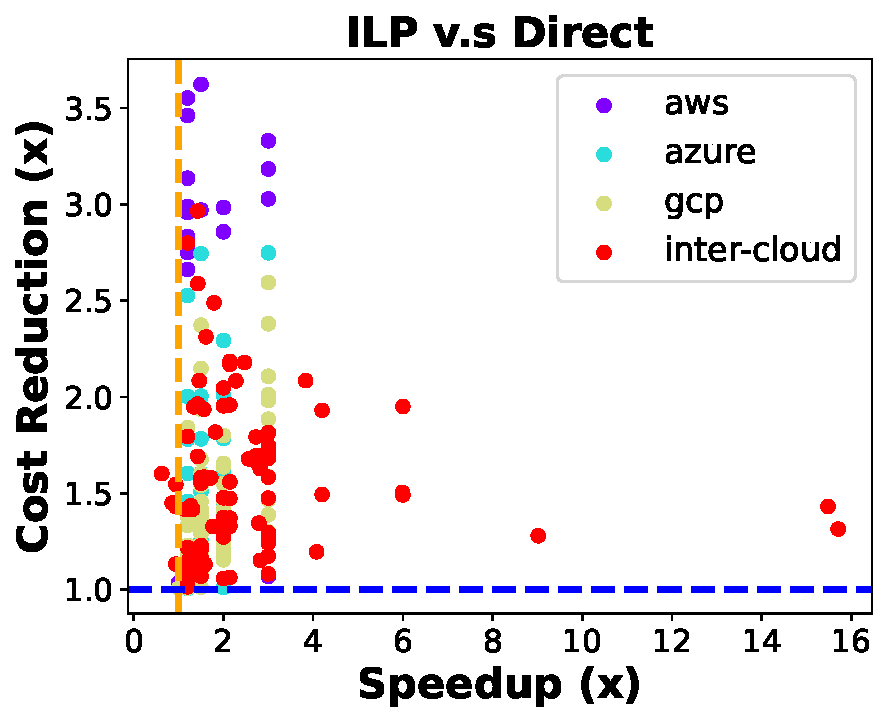
\includegraphics[width=.75\linewidth]{figures/6_dest_100_config.pdf}
%     \caption{\textbf{Simulation: 6 destinations, randomly sampled 100 configurations for Intra-aws/azure/gcp and Inter-cloud transfer)}}
%     \label{fig:random-6-dest}
% \end{figure}


% \begin{figure}[t]
%     \centering
%     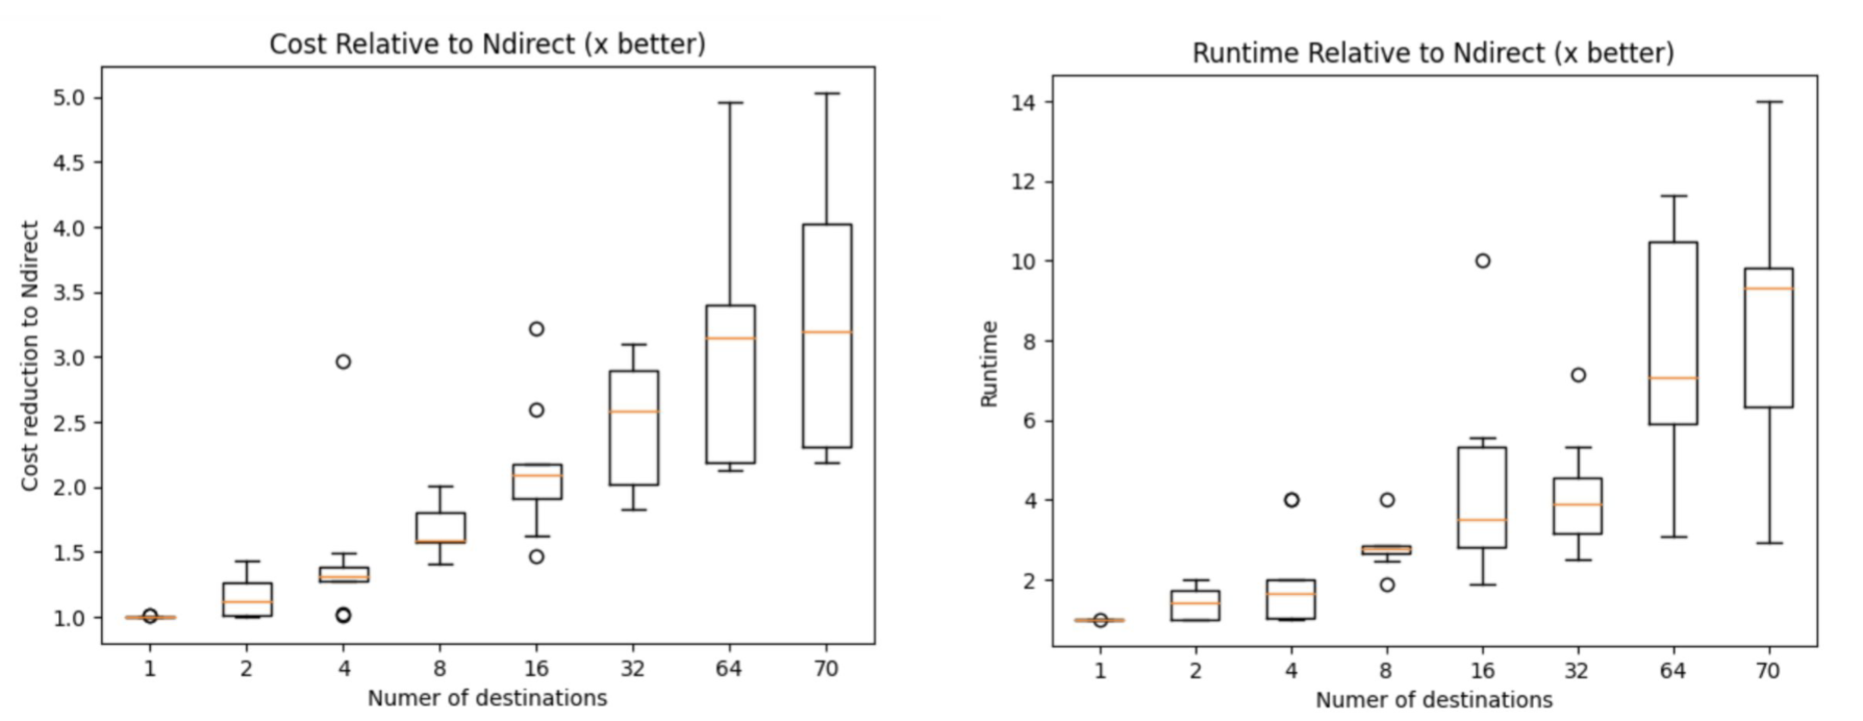
\includegraphics[width=.5\linewidth]{figures/dest_ablation.pdf}
%     \caption{\sys{} optimizer's cost and runtime improvement over direct replication for randomly sampled source and destination regions for varying numbers of destinations.} \label{fig:dest_ablation}
%     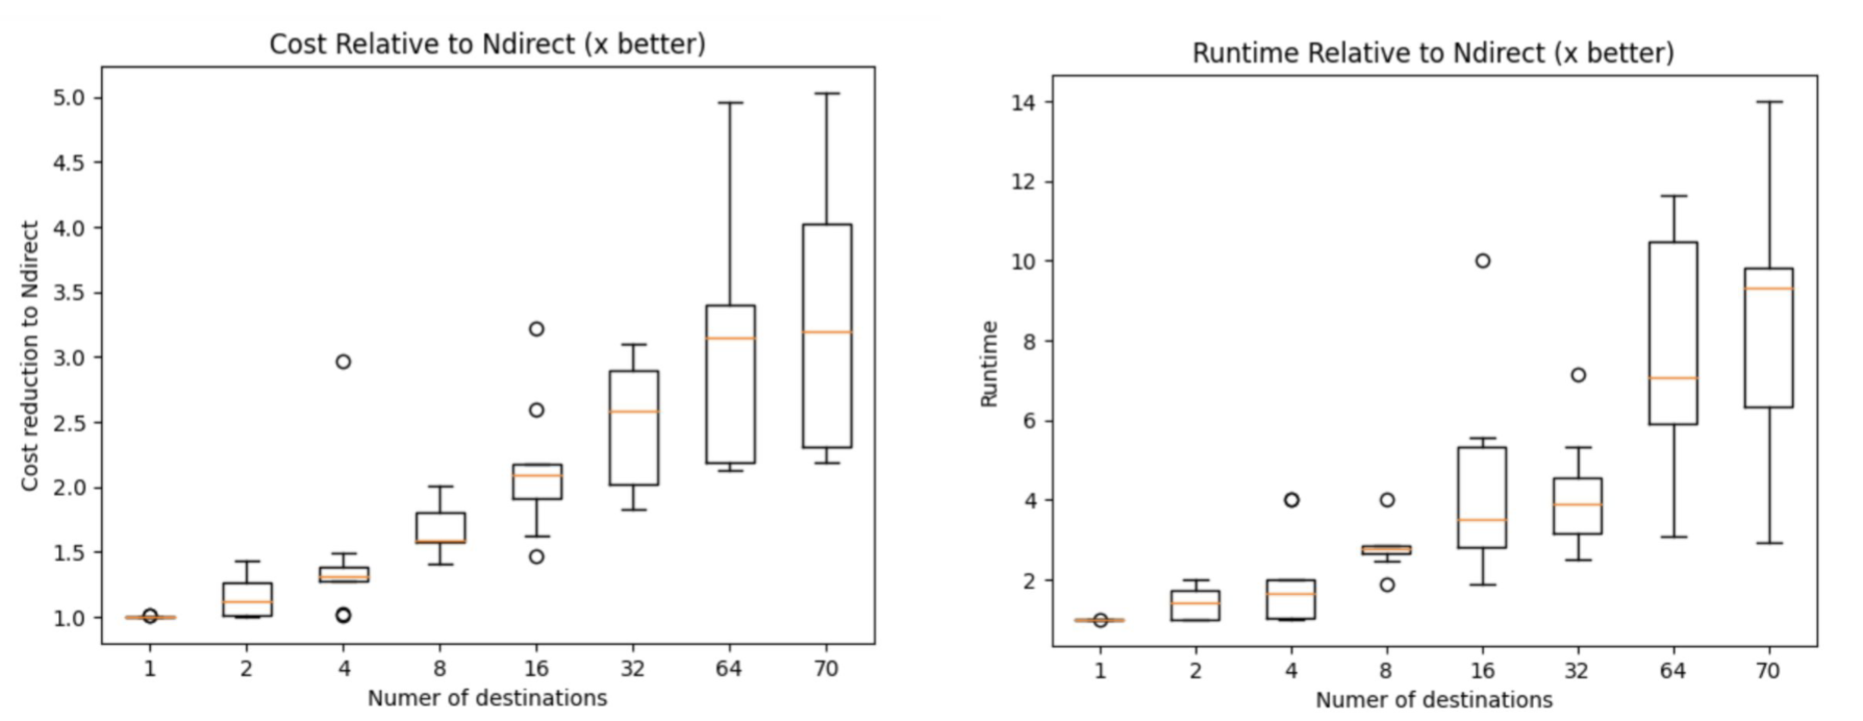
\includegraphics[width=.5\linewidth]{figures/dest_ablation.pdf}
% \end{figure}


\begin{figure}[t]
\centering
\subfloat[][Cost Reduction]{
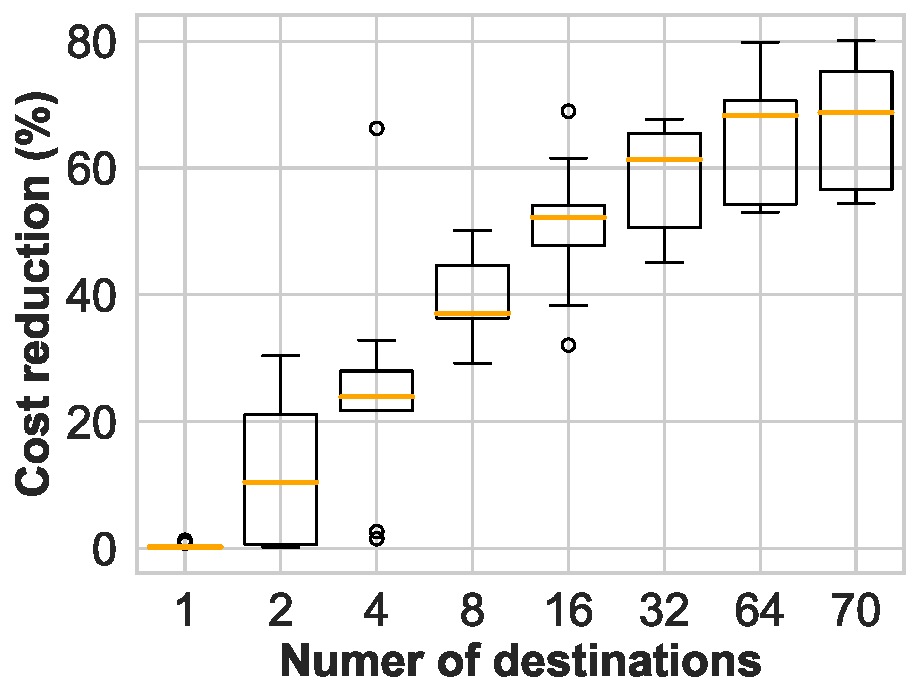
\includegraphics[width=.5\linewidth]{figures/ilp_vary_dest_ndirect_cost_reduction.pdf}\label{fig:dest_ablation1}
} 
\subfloat[][Replication Time Speedup]{
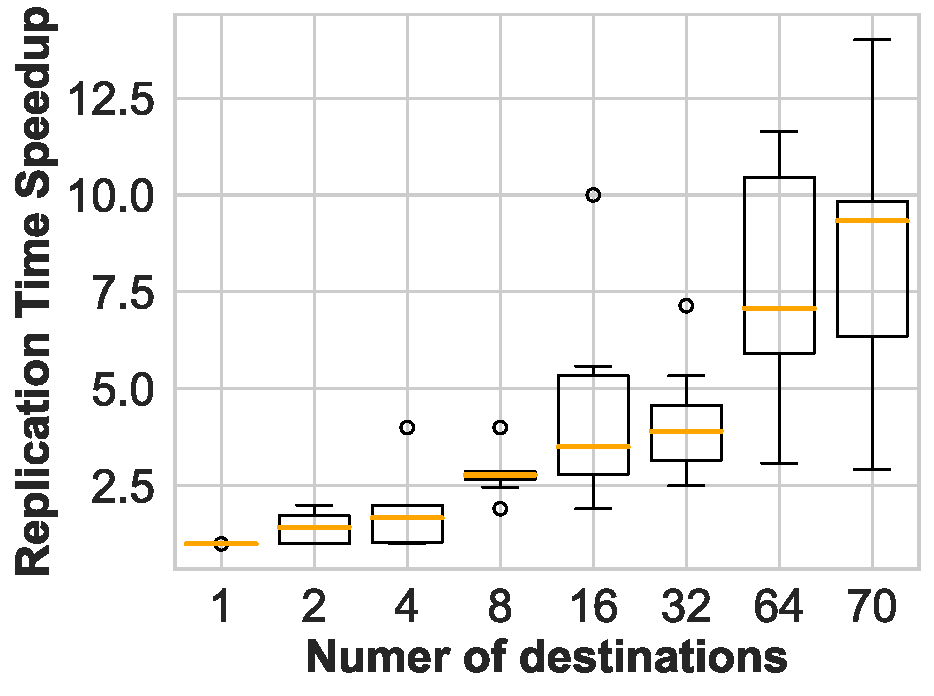
\includegraphics[width=.5\linewidth]{figures/ilp_vary_dest_ndirect_runtime_speedup.pdf}\label{fig:dest_ablation2}
}
\vspace{10pt} % Add extra space above the caption
\caption{\sys{} optimizer's cost and time improvement over direct replication with varying destination numbers.} \label{fig:dest_ablation}
\end{figure}

\subsubsection{Impact of approximations on solutions} 
\label{sss:solution_qual_eval}
% \label{sec:solution_qual_eval}
%As we described in \cref{ss:approximations}, the MILP formulation alone is not practical as a planning algorithm for \sys{} due to solver times that can take hours even for a few destinations. 

%We evaluate how our approximations (node filtering via clustering, hop constraining, and stripe iterative) affect both the solution quality and solver runtime. 

We evaluate how the optimizer with and without approximations scales to larger numbers of destinations in Figure~\ref{fig:solve_time}, by randomly selecting source and destination regions for varying numbers of destination regions. 
%We can see from Figure \ref{fig:solve_time} that 
We find that combining all three approximation mechanisms is necessary to scale the optimizer: using no approximations, or only one approximation, takes several minutes for just 10 destinations while using all approximations together reduces solve time to seconds. 

%For a given number of destinations, we sample a single random combination of source and destination regions, and measure the solver runtime with and without approximations, show in \cref{fig:solve_time}. We terminate the solver at 30 minutes if it cannot solve within that time. We find that we have to terminate the solver with no approximations with only 3 destinations. The stripe-iterative and node-clustering based approximations also can only run up to 7 and 14 destinations respectively and take 100s of seconds for higher numbers of destinations. However, if we combine all approximations together, we can solve for up to 20 destinations in a few seconds. 

\begin{figure}[t]
    \centering
    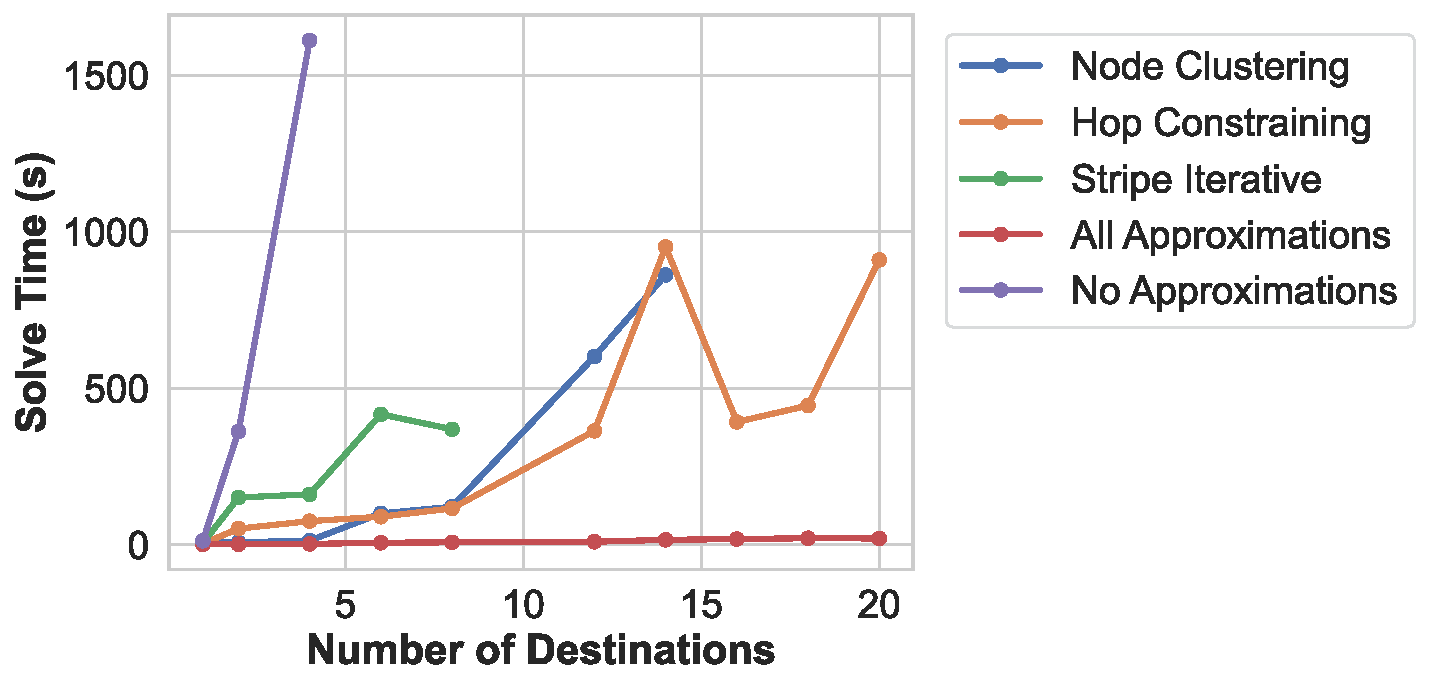
\includegraphics[width=0.9\linewidth]{figures/solve_time_versus_num_dest.pdf}
    \caption{Approximations reduce solver runtime from the cutoff of 30 minutes to seconds for up to 20 destinations.
    % We run the solver with different approximations mechanisms and cutoff measurement at 30 minutes. Without approximations (in purple), the solve time quickly become untenable and cannot reach beyond 4 destinations. With approximations (in red), solve time is within a few seconds even for up to 20 destinations.
    }
    \label{fig:solve_time}
\end{figure}

We also evaluate how approximations affect the quality of the solution using the monetary cost of the solver-generated solution. We randomly sample 100 source/destination combinations for 5 destinations and compute the difference in the solution's monetary cost and replication runtime compared to MILP without approximation in \cref{table:approx-quality}. We find that the difference in cost averages around $1\%$, and estimate the worst-case approximation ratio to be $1.4$. We find that for even just 5 destinations, the approximated solver runs with a geometric-mean speedup of $30.68\times$. %As such, our approximations are reliable and fast.


% \begin{table}[]
% \label{table2}
% \resizebox{\linewidth}{!}{%
% \begin{tabular}{|l|lll|lll|}
% \hline
% \multirow{2}{*}{Approximation} & \multicolumn{3}{l|}{Relative Solve Quality (\%)}               & \multicolumn{3}{l|}{Relative Solve Time Speedup (\times)}        \\ \cline{2-7} 
%                             & \multicolumn{1}{l|}{Min} & \multicolumn{1}{l|}{Max} & Avg & \multicolumn{1}{l|}{Min} & \multicolumn{1}{l|}{Max} & Avg \\ \hline
% \textit{Node Clustering}                        & \multicolumn{1}{l|}{-1.2}    & \multicolumn{1}{l|}{22.7}    &   1.00  & \multicolumn{1}{l|}{-2.5}    & \multicolumn{1}{l|}{50.7}    &   9.04 \\ \hline
% \textit{Hop Constraining}                        & \multicolumn{1}{l|}{-1.2}    & \multicolumn{1}{l|}{44.5}    &   1.01  & \multicolumn{1}{l|}{-0.72}    & \multicolumn{1}{l|}{26.2}    &   5.72 \\ \hline
% \textit{Stripe Iterative}                         & \multicolumn{1}{l|}{-0.4}    & \multicolumn{1}{l|}{0.8}    &   0.02  & \multicolumn{1}{l|}{-0.78}    & \multicolumn{1}{l|}{47.5}    &  7.02 \\ \hline
% \textit{All Approximations}                  & \multicolumn{1}{l|}{-1.7}    & \multicolumn{1}{l|}{\textbf{44.4}}    &  \textbf{1.08}  & \multicolumn{1}{l|}{-4.9}    & \multicolumn{1}{l|}{\textbf{219.1}}   &  \textbf{30.68}   \\ \hline
% \end{tabular}
% }
% \label{fig:approx-quality}
% \caption{Approximation Solve Time and Quality: Compare solution cost and solver runtime with respect to the original MILP for 100 randomly generated 5-destination configurations. Note that since the original MILP itself is an approximation, we are approximating an approximation, so the minimum is sometimes negative (i.e. it is not guaranteed the approximations result in worse solutions).}
% \end{table}
\begin{table}[t]
\centering
\small
\begin{tabular}{lcc}
\toprule
\textbf{Method} &
  \multicolumn{1}{c}{\textbf{Mean error}} &
  \multicolumn{1}{c}{\begin{tabular}[c]{@{}c@{}}\textbf{Solver speedup}\\ \textbf{(geomean)}\end{tabular}} \\ \midrule
\textit{Node Clustering}    & 0.3\% & 9.04$\times$  \\
\textit{Hop Constraining}   & 1.1\% & 5.72$\times$  \\
\textit{Stripe Iterative}   & 0.0\% & 7.02$\times$  \\
\cellcolor{Gray} \textit{All Approximations} & \cellcolor{Gray} 1.1\% & \cellcolor{Gray} 30.68$\times$ \\ \bottomrule
\end{tabular}%
\caption{Solve time and solution quality with approximations.}
\label{table:approx-quality}
\end{table}

%A challenge with making the optimizer practical for real-world use cases is having sufficiently low runtime even for large numbers of destinations and stripes. We reduce the runtime using approximation mechanisms described in \ref{reduce_optimizer_runtime}. We show how approximation mechanisms affect solver quality (in terms of the cost of the solution) and solver runtime in \cref{fig:approx-quality}. 


\subsubsection{Accuracy of replication time model}
\begin{table}[t]
\centering
\small
\begin{tabular}{cc}  
\toprule % Toprule applied here  
  
\textbf{Transfer Size (GB)} & \begin{tabular}[c]{@{}c@{}}\textbf{Prediction error}\end{tabular} \\  
  
\midrule % Midrule applied here  
   
 16 & 16.6\%\\  
 32 & 8.51\%\\  
 64 & 3.31\% \\  
 128 & 1.69\%\\  
\bottomrule % Bottomrule applied here  
\end{tabular}
\caption{Accuracy of the optimizer's predicted throughput.}
\label{table:tp-prediction}
\end{table} 

%Modeling replication throughput is key to ensuring optimizer solutions meet replication time constraints.
We compare optimizer-modeled throughput and real throughput in \cref{table:tp-prediction}.
As transfer size increases, the approximation becomes more accurate.
This is because \sys's optimizer, designed for bulk data replication, makes several simplifying assumptions, such as perfectly pipelined stripes.
Thus, transient inefficiencies during startup and teardown mean smaller transfers may experience lower throughput than the optimizer expects, but for larger, more expensive transfers, modeled throughput closely matches empirical results.

%For smaller transfers, throughput in \sys{} is less than what the optimizer models. However, for larger data transfers, the modeled expected throughput matches the real system throughput.

\subsection{When to Use \sys for Multicast?}
\sys is designed for bulk multicast replication in the cloud, so should only be used with data sizes are sufficiently large. Since \sys relies on creating VMs in the cloud at transfer initiation time, there is a constant overhead from VM startup time. We calculate the transfer size break-even point (i.e. the minimum data size for using \sys{}) for varying providers and VM capacity limits (constraining the throughput for the \sys overlay), shown in Figure~\ref{fig:size_threshold}. We approximate the per-destination replication throughput without \sys as equal to the per-VM egress bandwidth limit, ignoring congestion between source and destination VMs. Azure has a higher break-even point than AWS and GCP due to two effects. First, the VM startup time is the highest of all providers (56 seconds). Second, VMs in Azure are not subjected to egress constraints (5\ Gbps and 7\ Gbps for AWS and GCP, respectively). As a result, the benefits of using \sys's techniques are only realized for larger transfer sizes or larger numbers of destinations. 

\begin{figure}[t]
    \centering
    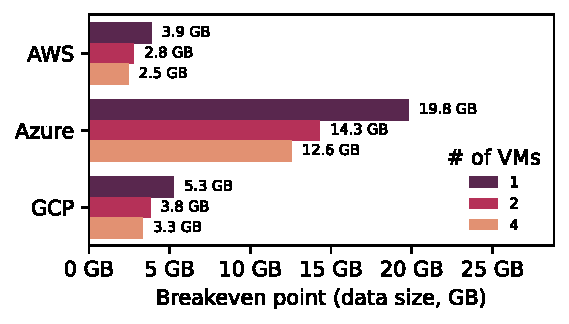
\includegraphics[width=0.7\linewidth]{figures/cloudflare_plot.pdf}
    \caption{Estimated break-even point for a 6-destination replication based on VM startup times ($35$, $56$, and $34$ seconds for AWS, Azure, and GCP, respectively) and VM egress limits. }
    \label{fig:size_threshold}
\end{figure}
%\vincent{what does incumbent mean here?  I would have thought AWS, as the biggest player in the space, is the `incumbent'?}
%\vincent{this is also a bit of a weird eval subsection.  perhaps it should be a section 7 discussion?}


\section{Related Work}

\topheading{Overlay Unicast} A significant body of prior work uses overlay networks to improve the performance and resilience of one-to-one data transfers in the Internet and peer-to-peer networks~\cite{andersen2001resilient, kostic2003bullet, castro2003splitstream}.
In clouds, previous work has also leveraged cloud elasticity to further improve performance~\cite{matos2009clon, jain2022skyplane}.
However, they do not consider multicast, and except Skyplane~\cite{jain2022skyplane}, none consider the monetary cost of replication in the cloud.
%\heading{Skyplane}
Handling multicast is challenging.
For example, while~\cite{jain2022skyplane} can leverage elastic resources, cloud pricing models, and overlay networking for bulk unicast replication in the cloud, its techniques are not directly applicable to the multicast setting.
More specifically, Skyplane's flow-based throughput model results in ambiguous multicast distribution tree solutions as it ignores the identity of data sent along multiple paths.
Furthermore, since Skyplane's optimizer is not designed for multicast, it cannot take advantage of techniques such as leveraging multiple distribution trees to alleviate source bottlenecks. 

\heading{Overlay Multicast}
% \todo{Provide reader with context on systems like Overcast, BDS, SplitStream, Bullet, etc.} 
End-system multicast~\cite{chu2002case} and overlay multicast have been proposed to efficiently disseminate data from a single source to multiple destinations. 
Many application-level multicast algorithms have been proposed. 
%Most of them are based on single or multiple multicast trees per sender. 
Algorithms like SPIDER~\cite{ganguly2005fast}, SplitStream~\cite{castro2003splitstream}, Bullet~\cite{kostic2003bullet}, and Overcast~\cite{jannotti2000overcast} are designed for high-bandwidth, cross-internet file distribution with application-level multicast overlays.
However, 
like with most overlay unicast systems, 
these algorithms ignore monetary costs and focus on techniques to maximize bandwidth. 

 \heading{Inter-DC Replication}
Extensive prior work addresses inter-DC replication~\cite{sima2022ekko, flinn2022owl, zhang2018bds, laoutaris2011inter, feng2012jetway}, including bulk multicast~\cite{luo2019deadline}. Recent research includes deadline~\cite{luo2019deadline} and cost-awareness~\cite{fatemipour2022cost, feng2012jetway}. However, the cost model in the Inter-DC setting cannot be easily adapted to cloud users, for which network pricing is based on total data volume rather than bandwidth.  Furthermore, existing formulations are not designed for multicast~\cite{fatemipour2022cost, feng2012jetway} or do not consider more than a few geo-distributed regions~\cite{luo2019deadline}.  Our work focuses on public clouds, considering unique per-GB network pricing, elastic resources, and cloud-specific resource constraints.  Our approximation algorithm is also designed to scale to all regions across multiple cloud vendors.

 \heading{Traffic Engineering}
The classic problem of traffic engineering has also formulated optimization problems for minimizing cost under performance constraints.
These techniques have recently been applied to cloud providers and their monetary costs.
For example, Entact~\cite{zhang2010optimizing} studied how to optimize costs for online service providers while still minimizing user latency.  
Similarly, Cascara~\cite{singh2021cost} leveraged latency-equivalent paths to identify cost-minimizing paths for cloud providers.
Like Inter-DC Replication, these approaches have been developed from the perspective of the cloud or service provider and, thus, present a materially different optimization problem.


\heading{Steiner Trees}
The Steiner Tree algorithm has been applied in the multicast setting both to minimize costs in terms of delay~\cite{jiang2016constructing} and cloud egress costs~\cite{garcia2015cost}).  CloudMPCast~\cite{garcia2015cost} minimizes egress costs in cloud bulk data multicast by constructing a Steiner Tree overlay network that avoids low-throughput cross-region paths.  However, CloudMPCast overlooks VM capacity and per-VM egress/ingress limits in its MILP formulation.  Also, CloudMPCast aims to achieve \textit{comparable} performance to direct transfers while minimizing cost, unlike \sys, which optimizes throughput. 


\heading{Geo-Distributed Storage}
Geo-distributed storage via data replication is supported by a variety of cloud services, such as AWS Cross-Region Replication~\cite{aws-replication}, AWS Multi-Region Access Points~\cite{aws-access-point}, and GCP Multi-region buckets~\cite{gcp-multi-region-bucket}.  Cross-region replicated buckets (e.g., S3 replication rules) automatically replicate written data from a bucket in one region to one or more buckets in other regions.  However, these services have limited support for cross-cloud data movement and do not minimize egress costs even for intra-cloud data movement.  SPANStore~\cite{wu2013spanstore} designs a system for geo-distributed storage across multiple cloud providers, and also optimizes egress costs of relaying data on PUT requests.  However, its relay strategy is optimized for latency, not bandwidth.  \shu{they actually do consider latency as an SLO constraint, same as ours; the difference is the resource limit constraint}

\heading{Peer-to-peer Multicast}
Peer-to-peer systems (P2P) support file sharing among a set of end-user clients.
% 
The BitTorrent protocol~\cite{cohen2003incentives} reduces the network load on the source by allowing clients to upload and download data to each other. 
% 
BitTorrent is widely used for data multicast in data center environments by Facebook~\cite{facebook-bittorrent} and Twitter~\cite{twitter-bittorrent}.
% 
Specialized systems for data multicast that use BitTorrent include Uber's Kraken~\cite{uber-kraken} and Ant Group's Dragonfly~\cite{dragonfly}.
% 
These P2P systems have significant overhead as they are designed for adversarial settings where peers may be unreliable or fail.
% 
Moreover, P2P systems must scale to millions of destinations and therefore lack centralized control which prevents custom routing topologies.
% 
P2P systems may redundantly send data over expensive links due to a lack of cost awareness. 

\begin{table}[tb]
	\footnotesize
	\begin{center}
        		\resizebox{\columnwidth}{!}{%
		\newcolumntype{P}[1]{>{\centering\arraybackslash}p{#1}}
		\begin{tabular}{@{}lccccc@{}}
			\toprule
\textsc{Method}   & \begin{tabular}{@{}c@{}}\textsc{Multicast} \\\end{tabular} & \begin{tabular}{@{}c@{}}\textsc{Cloud} \\ \textsc{Pricing}\end{tabular} & \begin{tabular}{@{}c@{}}\textsc{Striping} \end{tabular} & \begin{tabular}{@{}c@{}}\textsc{Resource} \\ \textsc{Elasticity}\end{tabular} \\
			\midrule
			\multicolumn{5}{@{}l}{\textbf{Unicast overlay networks}} \\
			RON~\cite{andersen2001resilient} & $\times$ & $\times$ & $\checkmark$ & $\times$\\
			Skyplane~\cite{jain2022skyplane} & $\times$ & $\checkmark$ & $\checkmark$ & $\checkmark$\\ 
                COMS~\cite{fatemipour2022cost}& $\times$  & $\times$ & $\times$ & $\sim$\\ 
			\midrule
			\multicolumn{5}{@{}l}{\textbf{Peer-to-peer}} \\
			BitTorrent~\cite{cohen2003incentives} & $\checkmark$ & $\times$ & $\checkmark$ & $\times$\\
			SplitStream~\cite{castro2003splitstream} & $\checkmark$ & $\times$ & $\checkmark$ & $\times$\\
			Bullet~\cite{kostic2003bullet} & $\checkmark$ & $\times$ & $\checkmark$ & $\times$\\
			\midrule
			\multicolumn{5}{@{}l}{\textbf{Inter-DC overlay multicast}} \\
			SPIDER~\cite{ganguly2005fast} & $\checkmark$ & $\times$ & $\checkmark$ & $\times$\\
			%QuickCast & TODO & TODO & TODO & TODO \\
			CodedBulk~\cite{tseng2021codedbulk} & $\checkmark$ & $\times$ & $\checkmark$ & $\times$\\
			BDS~\cite{zhang2018bds} & $\checkmark$ & $\times$ & $\checkmark$ & $\times$\\
                Deadline-aware Inter-DC~\cite{deadline2018} & $\checkmark$ & $\times$ & $\times$ & $\checkmark$ \\
			\midrule
			\multicolumn{5}{@{}l}{\textbf{Cost optimized overlay networks}} \\
			SPANStore~\cite{wu2013spanstore} & $\checkmark$ & $\checkmark$ & $\times$ & $\times$\\
            CloudMPCast~\cite{garcia2015cost} & $\checkmark$ & $\checkmark$ & $\times$ & $\times$\\
            Jetway~\cite{feng2012jetway} & $\times$ & $\checkmark$ & $\checkmark$ & $\times$ \\
            \midrule
			\rowcolor{Gray} \sys (ours) & $\checkmark$ & $\checkmark$ & $\checkmark$ & $\checkmark$\\ 
			\bottomrule
		\end{tabular}
  }
	\end{center}
	\caption{\sys{} builds on prior work by enabling multicast, optimizing cloud costs, and leveraging cloud resource elasticity and multiple distribution trees.}
	\label{tab:updated_baselines}
\end{table}

\section{Conclusion}
In this paper, we explored the problem of cost-optimized cloud multicast by introducing overlay networks of ephemeral VM waypoints that exploit path-specific cloud pricing to significantly reduce cost and improve throughput.
We developed a MILP formulation of this problem and introduced approximations that make the solving time feasible for practical applications. 
%We demonstrated that these approximations result in $30.68\times$ speedup in solve time with similar solution quality.
%To instantiate our multicast overlay network of ephemeral VMs we developed the Cloudcast system around our MILP formulation. 
Our evaluation against academic and commercial baselines demonstrated up to a $61.5\%$ reduction in cost and a $2.3\times$ improvement in runtime. 
\sys{} has been released as part of the Skyplane open source project  with pluggable planning algorithms to enable future research in this space.


\section*{Acknowledgments}
This work was supported by gifts from Accenture, AMD, Anyscale, Google, IBM, Intel, Microsoft, Mohamed Bin Zayed University of Artificial Intelligence, Samsung SDS, SAP, Uber, and VMware. We also thank Asim Biswal for his contributions to the open source artifact, and Daniel Rothchild for providing feedback on writing. 

%-------------------------------------------------------------------------------
\bibliographystyle{plain}
\bibliography{reference}

\appendix
%\section{Discussion}

\subsection{How does egress pricing affect multicast topologies?}
Different egress pricing models impact the generated multicast topologies. For example, Cloudflare R2 \cite{https://www.cloudflare.com/products/r2/} provides zero egress fee object storage. One can imagine putting the replicated data in Cloudflare R2 and reading it from multiple endpoints. In this way, we only need to pay the egress fee once for moving data out from the source instead of paying it repeatedly for multiple destinations. 
\shu{Should extend the discussions to talk about 1) how do we select cost-optimal topology now? are there any insights? 2) how will future changes in cloud pricings affect the cost-optimal topology (include Cloudflare, IBM free egress inter-region here)}

\subsection{Failures and Straggler Mitigation}
In \sys{}'s setting, the sockets can have very different rates of sending data over the network due to \cite{}. We have implemented a few mechanisms on top of \sys{} to mitigate stragglers. \shu{we might add measurements of this} There are other scenarios where failures might occur. For example, a VM might fail during the course of the transfer. 

% \subsection{Solver ablations}
% Should move some of the graphs for the solver studies here 
\section{Optimizer Parameters}

\subsection{Stripe Granularity}
The number of stripes is a parameter in the optimizer that determines the unit of data size that the optimizer determines routes. Choosing too small a number of stripes (e.g., 1-4) can result in solution infeasibility, since an individual stripe may be too large to fit along any given link under a replication time constraint.
% \ion{Why is that? In fact capacity and stripe size are not even comparable, one is measured in Gbps, and the other one in GB!} 
We show the tradeoff in \ref{fig:stripe-quality} between solution quality (dollar cost) and the number of stripes set of solving a 3-destination topology. Adding more stripes can increase the solver runtime unnecessarily. We use $8-16$ stripes for experiments. 

\begin{figure}[ht]
    \centering
    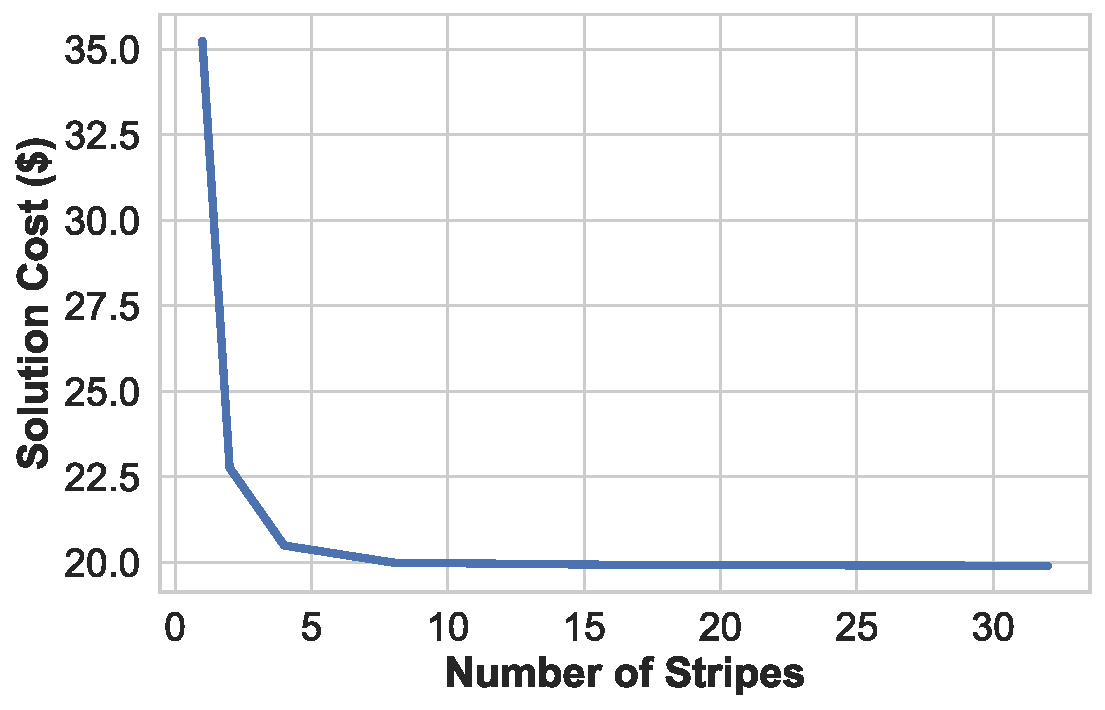
\includegraphics[width=.85\linewidth]{figures/num_stripes_quality.pdf}
    
    \caption{\textbf{Solution quality v.s the number of stripes.} Given a 6-destination intra-AWS transfer job and the same runtime SLO, our optimizer generates different solutions for different numbers of stripes. Small numbers of stripes can result in no feasible solution or solution with worse quality (i.e., higher cost). However, increasing the number of stripes to larger than 10 has diminishing returns.}  
    
    \label{fig:stripe-quality}
\end{figure} 

\subsection{Node Sub-Selection}
In Figure \ref{node-filtering}, we describe how we cluster nodes to select a subset of nodes for consideration by the optimizer. We motivate this by running an experiment to randomly select a subset of nodes in Figure \ref{fig:node_selection}. Generally, there are diminishing returns (beyond 20 nodes) to consider additional nodes. To avoid variability from randomness, we use the techniques described in  Figure \ref{fig:node_selection} to select a represented subset of nodes. 

\begin{figure}[ht]
     % \centering
     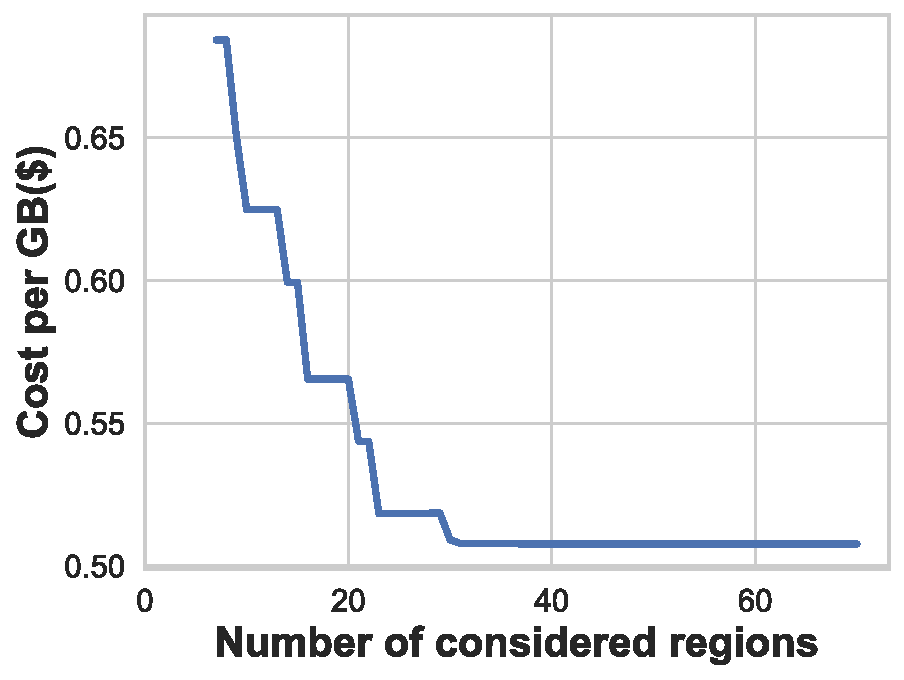
\includegraphics[width=.65\linewidth]{figures/node_sensitivity.pdf}
     \caption{Solution quality versus the number of considered nodes. Considering a larger set of regions has diminishing returns of solution quality but exponentially increases optimizer runtime. \shu{can move this graph to either the appendix, or replace it by \# of cluster ablations}}
     \label{fig:node_selection}
\end{figure}


\section{Formulation Details}
\label{s:formulation-details}

\subsection{Ensuring Valid Paths}
We cannot ensure connectivity of prevent cycles in paths defined by $\indicator$ without adding an exponential number of constraints. We define a special flow variable $\flow$ to add constraints that ensure that flow can be pushed along paths from $\indicator$ from the source to all destinations.\ion{I really think that for the entire subsection~\ref{sec-optimizer} we need to have a working example and refer to it throughout the section. Otherwise, it is hard to follow, like this para!}  The source node is denoted as the source region index in the transfer, the destination nodes are denoted as the destination region indices, and the sink node is denoted as a special node that is only connected to destination nodes. 
%
We constrain $\flow$ to have flow~\ion{What does it mean "$\flow$ to have flow"?} if and only if the corresponding stripe and edge for $\indicator$ is set to $1$. 
\begin{equation}
    \flow_{s, (u,v)}  \ge 1, \text{ if } \indicator_{s,(u,v)} = 1
\end{equation}
We ensure zero or negative flow 
\joey{I am confused, why would we have negative flow? What does that mean? Is the reverse of a flow negative?}
for $\indicator_{s,u,v} = 0$ via capacity constraints. We set special capacity constraints between destination nodes and the sink, to ensure that the sink can only receive sufficient flow if it receives flow from all destinations. 
\joey{I am having trouble getting an intuition for flow. Can you provide more high-level intuition?}\ion{Where is $\dest$ defined? I assume is the set of destinations. And, yes, the definition is confusing. Again, and running example in this section would help a lot.} 
\begin{equation}
    \flow_{s, (u, v)} \le 
\begin{cases}
    1,& \text{if } u\in \dest, v= \text{sink} \\
    0,& \text{if } \indicator_{s,(u,v)} = 0 \\
    |\dest|,              & \text{otherwise}  
\end{cases}
\end{equation}
We impose conservation of flow $\forall s$:\ion{Hard to reconcile above and below equations.}  
\begin{equation}
    \sum_{u\in V} \flow_{s, (u, v)} = 
\begin{cases}
    |\dest|,& \text{if $v$ is the source \shu{Why v?}} \\
    -|\dest|,              & \text{if $v$ is the sink}  \\
    0,              & \text{otherwise}
\end{cases}
\end{equation}
\joey{It occurs to me, is this graph directed?  Does $F_{s,u,v} = -F_{s,v,u}$?}
\joey{I really think this entire sub-section (5.2) should start with the idea that we will frame this problem as a MILP on a directed graph (or something).}
If the above constraints are met, this ensures that the stripe paths assigned by $\indicator$ are able to push flow from the source to all destinations. 

\subsubsection{Full Formulation}
We can write a full formulation of an integer linear program as the following: 
\begin{flalign}
& \argmin_{\indicator,\instances, \flow}  \runtime * \frob{\costi} \instances + \sum_s  \frob{\coste} \indicator \\
    & \instances \le \maxinstances \\
    & \stripesize * \sum_{s} \indicator_{s,(u, v)} \le \capacitye_{u, v} \\
    & \stripesize * \sum_{s}\sum_{u\in V} \indicator_{s, (v, u)} \le \capacityiegress \\
    & \stripesize * \sum_{s}\sum_{v\in V} \indicator_{s, (v, u)} \le \capacityiingress \\
    & \flow_{s, (u, v)}  \ge 1, \text{ if } \indicator_{s,(u,v)} = 1 \\
    & \sum_{u\in V} \flow_{s, (u, v)} = 
\begin{cases}
    |\dest|,& \text{if $v$ is the source} \\
    -|\dest|,              & \text{if $v$ is the sink}  \\
    0,              & \text{otherwise}
\end{cases} \\
    & \flow_{s, (u, v)} \le 
\begin{cases}
    1, &\text{if } u\in \dest, v= \text{sink} \\
    0, &\text{if } \indicator_{s,(u,v)} = 0 \\
    |\dest|,              & \text{otherwise}  
\end{cases}
\end{flalign}



%  \begin{figure}[t]
%      \centering
%      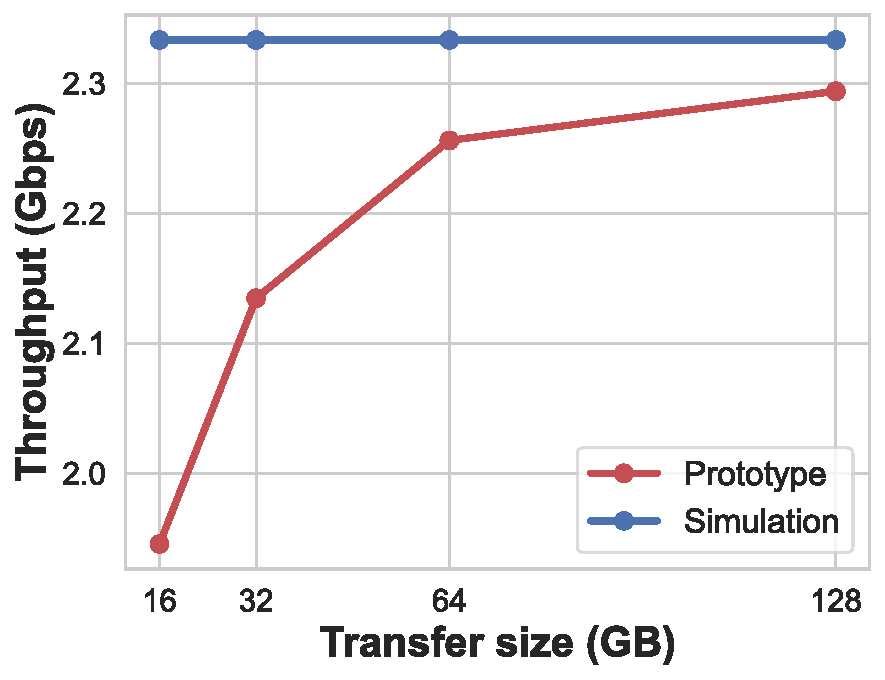
\includegraphics[width=.75\linewidth]{figures/new_simulator_accuracy.pdf}
%      \caption{Actual throughput v.s Predicted throughput: Throughput profiles can be used to accurately predict the throughput of data distribution trees. Here
% shows the result of the simulation and prototype through-
% put comparisons for 6-dest transfer \sarah{make this percentage} \sarah{DUPLICATE WITH TABLE}
%      }\label{fig:simulator_accuracy}
% \end{figure}

\section{How does Cheaper Egress Affect \sys's Optimizations?}
Some existing cloud providers (e.g., Cloudflare \cite{cloudflareegress}, Wasabi \cite{wasabi}, and Blackblaze \cite{blackblaze}) offer discounted or even free network egress.
Interestingly, incorporating free-egress clouds into \sys offers further opportunities to reduce costs.
Figure \ref{fig:cloudflare} illustrates this effect.
This highlights the importance of using a system like \sys, which can adapt replication plans in response to cheaper network offerings.

It is possible that major cloud providers will also adapt free-egress models or, in a less extreme case, make intra-cloud network fees more uniform as they build up additional capacity for inter-region networks with limited bandwidth. In this case, the techniques used by \sys{} (overlay networking, VM parallelism, and striping) would achieve only substantial throughput improvements but no cost improvement.

% \begin{figure}[t!]
%     \centering
%     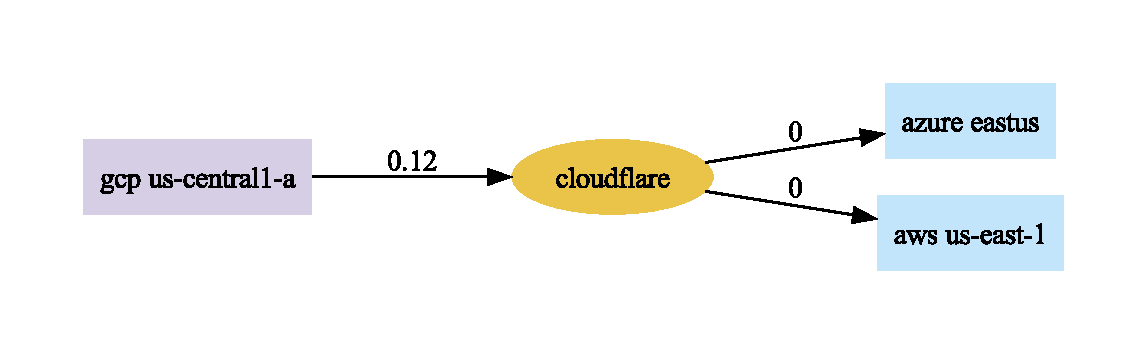
\includegraphics[trim=1cm 1.25cm 1cm 1.25cm, clip, width=\linewidth]{figures/cloudflare.pdf}
%     \caption{Routing data through free-egress clouds (e.g., Cloudflare): Inter-cloud egress only needs to be paid \textit{once} rather than a minimum of \textit{twice} to replicate data across three cloud providers (AWS, GCP, and Azure).}
%     \label{fig:cloudflare}
% \end{figure}

% \begin{table}[tbp]
% \caption{For the example in Figure~\ref{fig:cloudflare}, it is 2$\times$ cheaper to route via Cloudflare with Cloudcast.}
% \begin{tabular}{|l|l|l|l|}
% \hline
%  & \textbf{Direct} & \textbf{Cloudcast} & \textbf{\begin{tabular}[c]{@{}l@{}}Cloudcast \\ (with Cloudflare)\end{tabular}} \\ \hline
% \textbf{Cost (\$/GB)} & 0.24 & 0.2075 & 0.12 \\ \hline
% \end{tabular}
% \end{table}

\begin{figure}[ht!]
    \centering
    \begin{subfigure}[t]{0.5\textwidth}
        \centering
        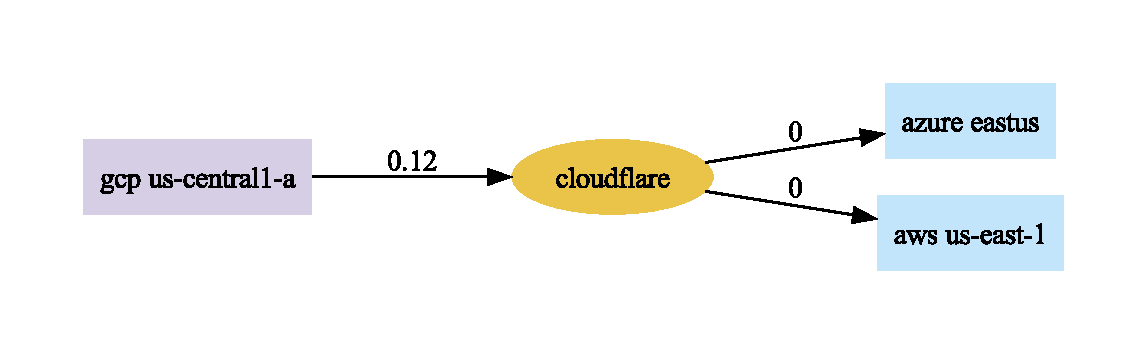
\includegraphics[trim=1cm 1.25cm 1cm 1.25cm, clip, width=\linewidth]{figures/cloudflare.pdf}
        \caption{Example of routing via no egress fee clouds.}
        \label{fig:cloudflare}
    \end{subfigure}

    \vspace{8pt}

    \begin{subfigure}[t]{\columnwidth}
        \centering
        \small
        %\resizebox{\textwidth}{!}
        \caption{Egress cost is 2$\times$ cheaper including Cloudflare in Cloudcast.}
        \label{tab:cloudcast}
    \end{subfigure}

    \vspace{8pt}
    
    \caption{Routing data through clouds with no egress fees (e.g., Cloudflare) can reduce inter-cloud replication costs as egress fees need to be paid only \textit{once} rather than a minimum of \textit{twice} to replicate data across AWS, GCP, and Azure.}
    \label{fig:table_figure}
\end{figure}
%%%%%%%%%%%%%%%%%%%%%%%%%%%%%%%%%%%%%%%%%%%%%%%%%%%%%%%%%%%%%%%%%%%%%%%%%%%%%%%%
\end{document}
%%%%%%%%%%%%%%%%%%%%%%%%%%%%%%%%%%%%%%%%%%%%%%%%%%%%%%%%%%%%%%%%%%%%%%%%%%%%%%%%

%%  LocalWords:  endnotes includegraphics fread ptr nobj noindent
%%  LocalWords:  pdflatex acks